\documentclass[12pt,a4paper]{article}
% ============================================================
%  Preamble dung chung cho de cuong NCKH sinh vien - RelyFetal
%  Bien dich bang: xelatex (2 lan) de co muc luc va tham chieu cheo
% ============================================================
\usepackage{fontspec}
\usepackage{polyglossia}
\setdefaultlanguage{vietnamese}
\setotherlanguage{english}
\setmainfont{Times New Roman}[Ligatures=TeX]
\setsansfont{Arial}
\setmonofont{Consolas}[Scale=0.88]

\usepackage[a4paper,top=2.5cm,bottom=2.5cm,left=3cm,right=2cm]{geometry}
\usepackage{amsmath,amssymb}
\usepackage{booktabs}
\usepackage{longtable}
\usepackage{array}
\usepackage{tabularx}
\usepackage{multirow}
\usepackage{makecell}
\usepackage{graphicx}
\usepackage{xcolor}
\usepackage{colortbl}
\usepackage{enumitem}
\usepackage{fancyhdr}
\usepackage{titlesec}
\usepackage{caption}
\usepackage{float}
\usepackage[hidelinks,bookmarksnumbered]{hyperref}
\usepackage{bookmark}
\usepackage{setspace}
\usepackage{ragged2e}
\usepackage{tcolorbox}
\tcbuselibrary{skins,breakable}

% ---------- mau ----------
\definecolor{tdtblue}{HTML}{1F3864}
\definecolor{tdtgray}{HTML}{5A5A5A}
\definecolor{rowbg}{HTML}{EFF3F8}
\definecolor{okgreen}{HTML}{1E6B33}
\definecolor{warnred}{HTML}{9B1C1C}
\definecolor{boxbg}{HTML}{F5F7FA}

% ---------- giai bay trang ----------
\onehalfspacing
\setlength{\parindent}{1.2em}
\setlength{\parskip}{3pt}
\sloppy
\hyphenpenalty=10000
\exhyphenpenalty=10000

% ---------- tieu de muc ----------
\titleformat{\section}{\normalfont\Large\bfseries\color{tdtblue}}{\thesection.}{0.6em}{}
\titleformat{\subsection}{\normalfont\large\bfseries\color{tdtblue}}{\thesubsection.}{0.6em}{}
\titleformat{\subsubsection}{\normalfont\normalsize\bfseries}{\thesubsubsection.}{0.6em}{}
\titlespacing*{\section}{0pt}{14pt}{7pt}
\titlespacing*{\subsection}{0pt}{11pt}{5pt}
\titlespacing*{\subsubsection}{0pt}{9pt}{4pt}

% ---------- dau trang chan trang ----------
\pagestyle{fancy}
\fancyhf{}
\renewcommand{\headrulewidth}{0.4pt}
\fancyhead[L]{\footnotesize\color{tdtgray} Đề cương NCKH sinh viên --- RelyFetal}
\fancyhead[R]{\footnotesize\color{tdtgray} Trường Đại học Tôn Đức Thắng}
\fancyfoot[C]{\thepage}

% ---------- bang ----------
\renewcommand{\arraystretch}{1.28}
\captionsetup[table]{font=small,labelfont=bf,skip=5pt}
\captionsetup[figure]{font=small,labelfont=bf,skip=5pt}
\newcolumntype{L}[1]{>{\RaggedRight\arraybackslash}p{#1}}
\newcolumntype{C}[1]{>{\Centering\arraybackslash}p{#1}}
\newcolumntype{R}[1]{>{\RaggedLeft\arraybackslash}p{#1}}

% ---------- hop ghi chu ----------
\newtcolorbox{ghichu}[1][]{
  enhanced,breakable,colback=boxbg,colframe=tdtblue,
  boxrule=0.5pt,left=8pt,right=8pt,top=6pt,bottom=6pt,
  fonttitle=\bfseries\small,coltitle=white,
  attach boxed title to top left={yshift=-2mm,xshift=6mm},
  boxed title style={colback=tdtblue,boxrule=0pt,arc=1pt},#1}

\newtcolorbox{canhbao}[1][]{
  enhanced,breakable,colback=white,colframe=warnred,
  boxrule=0.7pt,left=8pt,right=8pt,top=6pt,bottom=6pt,
  fonttitle=\bfseries\small,coltitle=white,
  attach boxed title to top left={yshift=-2mm,xshift=6mm},
  boxed title style={colback=warnred,boxrule=0pt,arc=1pt},#1}

% ---------- lenh tat ----------
\newcommand{\tot}[1]{\textcolor{okgreen}{\textbf{#1}}}
\newcommand{\xau}[1]{\textcolor{warnred}{\textbf{#1}}}
\newcommand{\mh}{\textsc{FetalQRS-TCN}}
\newcommand{\hethong}{\textsc{RelyFetal}}


\title{Đề cương nghiên cứu khoa học sinh viên --- RelyFetal}
\author{Ngô Bình Minh}
\date{12/09/2026}

\begin{document}

% ============================================================ TRANG BÌA
\begin{titlepage}
\centering
\setstretch{1.0}
\vspace*{0.1cm}

{\large TRƯỜNG ĐẠI HỌC TÔN ĐỨC THẮNG}\\[2pt]
{\large KHOA CÔNG NGHỆ THÔNG TIN}\\[1.0cm]

{\Large\bfseries ĐỀ CƯƠNG NGHIÊN CỨU KHOA HỌC SINH VIÊN}\\[0.3cm]
{\large Năm học 2026 --- 2027}\\[1.1cm]

\rule{\textwidth}{0.8pt}\\[0.5cm]
{\LARGE\bfseries\color{tdtblue} Dò phức bộ QRS thai nhi từ điện tim ổ bụng đơn kênh có nhận biết độ tin cậy\par}
\vspace{0.35cm}
{\large Đối chuẩn không rò rỉ giữa các họ biểu diễn tín hiệu\\ và chỉ số chất lượng dựa trên đồng điều bền vững\par}
\vspace{0.45cm}
\rule{\textwidth}{0.8pt}\\[0.4cm]

{\normalsize\itshape Reliability-aware single-channel fetal QRS detection:\\
a leakage-free representation benchmark and a persistent-homology signal-quality index\par}
\vspace{0.9cm}

\begin{tabular}{@{}r@{\hspace{1.2em}}l@{}}
\textbf{Tên hệ thống}      & \textsc{RelyFetal} \\[3pt]
\textbf{Chủ nhiệm đề tài}  & Ngô Bình Minh \\[3pt]
\textbf{Nhóm thực hiện}    & 03 sinh viên \\[3pt]
\textbf{Thời lượng}        & 24 tuần \\[3pt]
\textbf{Phiên bản}         & 3.4 --- 12/09/2026 \\[3pt]
\textbf{Mục tiêu công bố}  & \makecell[l]{01 tạp chí Q1 (\textit{Physiological Measurement} /\\ \textit{Biomed.\ Signal Process.\ Control} / \textit{IEEE JBHI})\\ 01 hội nghị \textit{Computing in Cardiology}\\ 01 báo cáo Euréka} \\
\end{tabular}

\vfill

\begin{ghichu}[title={Điểm khác biệt của bản đề cương này}]
\footnotesize
\justifying
Đây không phải một bản kế hoạch thuần lý thuyết. Trước khi viết, nhóm đã chạy hơn 600.000 cửa sổ
tín hiệu, huấn luyện và lưu hơn hai mươi mô hình, đọc toàn văn 30 công trình,
và \textbf{tự bác bỏ giả thuyết trung tâm của chính bản đề cương phiên bản đầu tiên}.
Mọi con số trong tài liệu này đều do nhóm tự đo, có mã nguồn và nhật ký kèm theo, và chạy lại được.
Những chỗ nhóm còn chưa chắc chắn được ghi rõ trong \S\ref{sec:phanbien}.

\smallskip
\textbf{Năm phát biểu đã bị rút công khai.} Bốn của bản 3.2: (i) con số CinC 2013 đo trên \textbf{mẫu 10
bản ghi} của một tập có 75 --- số đúng là 79,40 trên toàn bộ 75 (\S\ref{sec:cinc75}); (ii) ``Power-MF
không chạy lại được'' --- sai, đã chạy (\S\ref{sec:powermf}); (iii) mọi trị số $p$ trên 5 sản phụ là giả
lập và đã bị gỡ, ``8 kiến trúc không phân biệt được'' đổi thành ``không đủ lực để phân biệt''
(\S\ref{sec:thongke}); (iv) hệ thống \textbf{chưa} dùng được làm máy đo biến thiên ngắn hạn
(\S\ref{sec:clinical}).

\smallskip
\textbf{Và một của chính bản 3.3, rút chiều 12/09:} con số Power-MF 94,87 cùng kết luận ``loại hai bản
ghi bắt cách nhịp thì còn 98,38 so với 97,33'' \textbf{đều sai}. Cả hai đứng trên một bản Octave hỏng vì
\textit{lỗi cổng chuyển của chính nhóm} (\texttt{findpeaks} tốn $O(k^2)$ bộ nhớ), không phải vì tham số
340\,ms như nhóm đã đoán --- giả thuyết đó bị bác bỏ bằng số đo: 0,00\,\% khoảng RR dưới 340\,ms. Sau khi
vá, Power-MF đa kênh đạt \textbf{98,83} và tái lập số công bố của tác giả đến 0,06 điểm
(\S\ref{sec:powermf}). Hai lần đoán sai nguyên nhân trong cùng một ngày được phân tích ở
\S\ref{sec:doansai}.
\end{ghichu}

\vspace{0.5cm}
{\small Thành phố Hồ Chí Minh --- Tháng 9 năm 2026}
\end{titlepage}

% ============================================================ MỤC LỤC
\pagenumbering{roman}
\tableofcontents
\clearpage
\listoftables
\listoffigures
\clearpage
\pagenumbering{arabic}

% ================================================================= 1. TÓM TẮT
\section{Tóm tắt}

Theo dõi tim thai không xâm lấn bằng \textbf{một} điện cực dán trên bụng mẹ là cấu hình rẻ nhất và
dễ đeo nhất cho giám sát tại nhà, đồng thời là cấu hình khó nhất về mặt xử lý tín hiệu. Sóng tim thai
bị sóng tim mẹ lớn gấp nhiều lần che khuất, hai nguồn trùng phổ tần số, và khi chỉ có một kênh thì
không dùng được các phương pháp tách nguồn mù đa kênh vốn cho kết quả tốt nhất.

Hai mươi năm nghiên cứu đã sinh ra hàng chục phương pháp với F1 công bố trải từ 77\% đến 99,7\%.
Nhóm đã đọc toàn văn 30 công trình và kết luận rằng \textbf{phần lớn các con số đó không so sánh
được với nhau}, vì chúng khác nhau ở cách tách chủ thể, dung sai ghép cặp, số kênh thực sự dùng, và
việc có tinh chỉnh trên tập đích hay không. Chi tiết ở \S\ref{sec:yvan}.

Trước khi viết đề cương này, nhóm đã chạy một loạt thí nghiệm tiền khả thi. Ba kết quả định hình
toàn bộ phần còn lại của tài liệu.

\begin{enumerate}[leftmargin=1.5em,itemsep=4pt]
\item \textbf{Front-end tín hiệu quan trọng hơn kiến trúc mạng rất nhiều.}
Chỉ đổi dải thông từ 1--45\,Hz sang 10--60\,Hz nâng macro F1 thêm \tot{11,00 điểm} trong cùng một
thí nghiệm có kiểm soát. Trong khi đó, khi giữ cố định ngữ cảnh thời gian, việc thay gradient boosting
bằng mạng học sâu chỉ đáng \xau{+0,41 điểm} với $p = 0{,}7012$, tức không có ý nghĩa thống kê.

\item \textbf{Biểu diễn topo không phù hợp cho bài toán dò đỉnh.}
Persistence Image kết hợp CNN 2D đứng \xau{cuối cùng trong 16 kiến trúc} được so ở cùng ngân sách
tham số (F1 27,42 so với 97,14 của CNN 1D cùng 27 nghìn tham số). Nhóm cũng chứng minh được bằng số
rằng đặc trưng $H_0$ của lọc dưới mức trên tín hiệu một chiều \textbf{trùng khớp 100\%} với độ nhô đỉnh
cổ điển, tức không phải một đặc trưng mới.

\item \textbf{Rào cản thật không phải độ chính xác trung bình mà là độ tin cậy.}
Mô hình của nhóm đạt macro F1 \tot{99,21} trên ADFECGDB khi tách theo bản ghi, nhưng khi chuyển sang
PhysioNet/CinC 2013 mà không tinh chỉnh thì chỉ còn \xau{77,34}. Quan trọng hơn con số trung bình là
hình dạng phân bố: bốn trên mười bản ghi đạt F1 tuyệt đối 100\%, ba bản khác sụp xuống dưới 50\%.
\textbf{Hệ thống không biết khi nào nó sai.}
\end{enumerate}

Từ ba quan sát đó, đề tài đề xuất \hethong{}: một bộ dò QRS thai đơn kênh \textbf{kèm chỉ số chất lượng
tín hiệu thai dựa trên đồng điều bền vững}, cho phép hệ thống \textbf{từ chối trả lời} khi tín hiệu
không đủ tin cậy, thay vì im lặng đưa ra một nhịp tim sai.

\begin{ghichu}[title={Ba đóng góp}]
\begin{description}[leftmargin=2.2em,style=nextline,itemsep=3pt]
\item[C1 --- Đối chuẩn không rò rỉ.] So sánh năm họ biểu diễn tín hiệu dưới cùng một giao thức,
cùng bộ phân loại, cùng ngân sách huấn luyện, trên ba bộ dữ liệu, với quy tắc chọn kênh
\textbf{mù nhãn} có thể đăng ký trước.
\item[C2 --- Phân rã đóng góp ba tầng.] Trả lời định lượng câu hỏi: trong toàn bộ pipeline, phần nào
thực sự tạo ra hiệu năng? Đây là xương sống khoa học của đề tài.
\item[C3 --- Chỉ số chất lượng tín hiệu thai dựa trên đồng điều bền vững, có quyền từ chối trả lời.]
Đây là ứng dụng đầu tiên của phân tích dữ liệu topo cho tín hiệu tim thai mà nhóm tìm được.
\end{description}
\end{ghichu}

\clearpage

% ================================================================= 2. ĐẶT VẤN ĐỀ
\section{Đặt vấn đề}

\subsection{Bối cảnh lâm sàng}

Nhịp tim thai và hình thái phức bộ QRS thai là cửa sổ chính để phát hiện suy thai, thiếu oxy và một số
bất thường tim bẩm sinh. Hai phương pháp đang dùng trên lâm sàng đều có hạn chế rõ ràng.

\begin{table}[H]\centering\small
\caption{Hai phương pháp theo dõi tim thai hiện hành và giới hạn của chúng.}
\label{tab:lamsang}
\begin{tabular}{@{}L{4.0cm} L{5.0cm} L{5.4cm}@{}}
\toprule
\textbf{Phương pháp} & \textbf{Ưu điểm} & \textbf{Giới hạn} \\
\midrule
Tim thai đồ / Doppler (CTG) & Không xâm lấn, phổ biến & Chỉ cho nhịp, không cho hình thái. Cần kỹ thuật
viên đặt đầu dò. Không dùng liên tục tại nhà được. \\
Điện cực xoắn da đầu thai & Chuẩn vàng, tín hiệu sạch & Xâm lấn. Chỉ dùng được sau khi đã chuyển dạ
và vỡ ối. Không dùng cho theo dõi thai kỳ. \\
\bottomrule
\end{tabular}
\end{table}

Điện tim thai không xâm lấn từ điện cực ổ bụng cho phép theo dõi liên tục, tại nhà, chi phí thấp, và
cho cả hình thái sóng chứ không chỉ nhịp. Cấu hình \textbf{đơn kênh} là rẻ nhất và dễ tích hợp vào đai
đeo nhất, nhưng cũng loại bỏ luôn khả năng dùng tách nguồn mù đa kênh --- vốn là họ phương pháp đạt độ
chính xác cao nhất trong đối chuẩn tổng hợp của Andreotti và cộng sự.

\subsection{Vì sao đơn kênh khó}

Bảng dưới đây là các con số nhóm \textbf{tự đo được} trên ADFECGDB, không phải trích từ y văn.

\begin{table}[H]\centering\small
\caption{Các khó khăn của cấu hình đơn kênh, kèm hệ quả định lượng nhóm đo được trên ADFECGDB.}
\label{tab:khokhan}
\begin{tabular}{@{}L{6.2cm} L{8.2cm}@{}}
\toprule
\textbf{Thách thức} & \textbf{Hệ quả định lượng} \\
\midrule
Biên độ sóng thai nhỏ hơn sóng mẹ nhiều lần & Tỉ số RMS giữa vùng QRS thai và nền chỉ \textbf{1,24}
ở dải 1--45\,Hz; lên \textbf{1,64} ở dải 15--60\,Hz \\
Trùng phổ tần số trong khoảng 0,5--40\,Hz & Lọc tuyến tính không tách được nếu không làm méo sóng thai \\
Nhịp mẹ và nhịp thai trùng pha & \textbf{17--19\%} nhịp thai nằm trong $\pm$60\,ms của một nhịp mẹ \\
Không có đa dạng không gian & Không dùng được tách nguồn mù đa kênh (ICA, PCA, $\pi$CA) \\
Chất lượng kênh biến thiên cực lớn & F1 theo từng kênh dao động từ \textbf{85,03} đến \textbf{100,00}
trên cùng một bản ghi \\
Dữ liệu có nhãn rất ít & ADFECGDB chỉ có 5 sản phụ; chia ngẫu nhiên là rò rỉ dữ liệu \\
\bottomrule
\end{tabular}
\end{table}

\subsection{Ba khoảng trống trong y văn}
\label{sec:khoangtrong}

Nhóm đã tải và đọc \textbf{toàn văn 30 công trình} (danh mục đầy đủ ở \S\ref{sec:yvan} và Phụ lục).
Ba khoảng trống được xác nhận.

\begin{description}[leftmargin=2.6em,style=nextline,itemsep=6pt]

\item[G1 --- Không có so sánh công bằng giữa các họ biểu diễn tín hiệu.]
Mỗi công trình dùng một biểu diễn riêng (tín hiệu thô, ma trận trễ, phổ đồ thời gian--tần số, đặc trưng
topo) trên dữ liệu riêng với giao thức riêng. Chưa có công trình nào giữ cố định đồng thời bộ phân loại,
dữ liệu, giao thức và ngân sách huấn luyện để so các biểu diễn. Hệ quả là cộng đồng không biết cải tiến
đến từ biểu diễn hay đơn giản là từ tiền xử lý tốt hơn.

\item[G2 --- Không có đánh giá độ tin cậy ở mức bản ghi.]
Mọi công trình đều báo cáo một con số F1 trung bình. Không công trình nào trả lời câu hỏi lâm sàng
thật sự: \textit{``với bản ghi cụ thể đang nằm trước mặt, đầu ra này có đáng tin không?''} Đo đạc của
nhóm cho thấy phân bố hiệu năng là \textbf{lưỡng cực}, nên chính con số trung bình đang che giấu thông
tin quan trọng nhất.

\item[G3 --- Chưa có công trình nào áp dụng đồng điều bền vững cho tín hiệu tim thai.]
Nhóm truy vấn có cấu trúc trên Europe PMC REST, Semantic Scholar, OpenAlex và arXiv API với tổ hợp
\texttt{("persistent homology" OR "topological data analysis" OR "persistence image") AND (fetal OR
foetal OR "abdominal ECG" OR cardiotocography)}, tìm bổ sung bằng tiếng Trung, tiếng Việt và tiếng
Tây Ban Nha. Không có kết quả nào là công trình về tín hiệu thai. Kết quả gần nhất là biến thiên nhịp
tim nhi khoa, mà chính tác giả nêu \textit{``mở rộng khung này sang fetal HRV''} là hướng tương lai.

\end{description}

\subsection{Câu hỏi nghiên cứu và giả thuyết}

\begin{table}[H]\centering\small
\caption{Sáu câu hỏi nghiên cứu và thí nghiệm trả lời tương ứng.}
\label{tab:rq}
\begin{tabular}{@{}C{1.1cm} L{10.6cm} L{2.5cm}@{}}
\toprule
\textbf{Mã} & \textbf{Câu hỏi} & \textbf{Thí nghiệm} \\
\midrule
RQ1 & Dưới một giao thức không rò rỉ, họ biểu diễn tín hiệu nào cho hiệu năng dò fQRS đơn kênh tốt nhất
khi giữ cố định bộ phân loại và ngân sách huấn luyện? & E1 \\
RQ2 & Trong toàn bộ pipeline, tầng nào đóng góp nhiều nhất: front-end tín hiệu, độ dài ngữ cảnh, họ
kiến trúc, hay hậu xử lý? & E2 \\
RQ3 & Chỉ số chất lượng dựa trên đồng điều bền vững có dự báo được khi nào bộ dò sẽ sai, và có tốt hơn
các chỉ số cổ điển (SampEn, bSQI, kurtosis, entropy phổ) không? & E3 \\
RQ4 & Cơ chế từ chối trả lời nâng độ tin cậy lên bao nhiêu, đánh đổi bằng bao nhiêu phần trăm dữ liệu
bị loại? & E4 \\
RQ5 & Hiệu năng suy giảm thế nào khi chuyển miền và khi tỉ số tín hiệu trên nhiễu giảm? & E5, E6 \\
RQ6 & Tiền huấn luyện trên dữ liệu tổng hợp rồi tinh chỉnh trên dữ liệu thật có cải thiện khả năng
tổng quát hoá không? & E7 \\
\bottomrule
\end{tabular}
\end{table}

\begin{table}[H]\centering\small
\caption{Giả thuyết kiểm định được và tiêu chí chấp nhận.}
\label{tab:h}
\begin{tabular}{@{}C{1.1cm} L{9.0cm} L{4.2cm}@{}}
\toprule
\textbf{Mã} & \textbf{Giả thuyết} & \textbf{Tiêu chí chấp nhận} \\
\midrule
H1 & Bộ dò \hethong{} đạt F1 $\geq$ 95\% trên ADFECGDB khi tách theo bản ghi, với quy tắc chọn kênh
mù nhãn & Wilcoxon ghép cặp so với nền trừ mẫu kết hợp PCA, $p < 0{,}05$ \\
H2 & Front-end tín hiệu đóng góp nhiều hơn họ kiến trúc ít nhất 5 lần về điểm F1 & So sánh hai hiệu ứng
chính, kèm khoảng tin cậy bootstrap \\
H3 & fSQI topo có tương quan Spearman $|\rho| \geq 0{,}6$ với F1 thực theo bản ghi, và không kém
SampEn & Bootstrap CI cho hiệu số $\rho$ \\
H4 & Từ chối 20\% dữ liệu có fSQI thấp nhất nâng F1 trên phần còn lại thêm $\geq$ 8 điểm & Đường cong
rủi ro--độ phủ, so với cổng từ chối ngẫu nhiên \\
H5 & Tiền huấn luyện FECGSYNDB nâng F1 xuyên bộ dữ liệu thêm $\geq$ 5 điểm & Wilcoxon ghép cặp theo
bản ghi \\
H0 & \textbf{Giả thuyết phủ định vẫn có giá trị}: nếu H3--H5 không đạt, thì đối chuẩn cộng phân rã
đóng góp cộng kết quả phủ định có kiểm định vẫn là một bài báo hoàn chỉnh & --- \\
\bottomrule
\end{tabular}
\end{table}

\clearpage

% ================================================================= 3. TỔNG QUAN Y VĂN
\section{Nhóm đã đọc gì và so với ai}
\label{sec:yvan}

Phần này trả lời trực tiếp câu hỏi mà một hội đồng sẽ đặt ra đầu tiên: \textit{nhóm đã đọc những gì,
và mô hình của nhóm đứng ở đâu so với các công trình đó?}

\subsection{Cách nhóm chọn và đọc}

Nhóm tải về và đọc \textbf{toàn văn 30 công trình}, không dừng ở phần tóm tắt. Danh mục được chọn theo
bốn tiêu chí: các công trình được trích dẫn nhiều nhất trong lĩnh vực dò QRS thai; các công trình mới
nhất giai đoạn 2024--2026; các công trình mô tả bộ dữ liệu và thử thách chuẩn; và toàn bộ nền tảng lý
thuyết của phân tích dữ liệu topo mà bản đề cương đầu tiên của nhóm dựa vào.

Khi đọc, nhóm ghi lại bảy điểm cho từng bài, vì đây là những chỗ quyết định một con số công bố có so
sánh được hay không.

\begin{enumerate}[leftmargin=1.6em,itemsep=2pt]
\item Giao thức tách dữ liệu: tách theo chủ thể, tách theo bản ghi, hay chia ngẫu nhiên?
Chia ngẫu nhiên trên cùng một bệnh nhân là \textbf{rò rỉ dữ liệu}.
\item Dung sai ghép cặp nhịp: 50\,ms là quy ước CinC 2013, 150\,ms là chuẩn AAMI EC57 cho người lớn.
Nới dung sai làm con số đẹp lên mà không cần cải tiến gì.
\item Dùng thật sự một kênh hay gộp nhiều kênh? Nhiều công trình tự nhận ``đơn kênh'' nhưng thực tế
gộp bốn kênh ở bước cuối.
\item Có tinh chỉnh trên tập đích không? Nếu có thì không so được với mô hình không tinh chỉnh.
\item Dải thông dùng là gì? Theo thực nghiệm của nhóm, đây là biến quan trọng nhất.
\item Độ dài cửa sổ ngữ cảnh là bao nhiêu giây?
\item Có báo cáo chi phí tính toán không? Nếu không thì công trình đó không tái lập được về mặt kỹ thuật.
\end{enumerate}

\subsection{Kết quả tổng hợp}

Trong 30 công trình, chỉ \textbf{bốn} công trình có giao thức đối chiếu trực tiếp được với giao thức của
nhóm. Phần lớn còn lại rơi vào một trong các trường hợp: chia ngẫu nhiên trong cùng chủ thể, dung sai
rộng hơn, gộp nhiều kênh, tinh chỉnh trên tập đích, hoặc đơn vị phân tích là cửa sổ tín hiệu thay vì
nhịp tim.

\begin{ghichu}[title={Phát hiện đáng chú ý nhất khi đọc y văn}]
Công trình học sâu nền tảng của lĩnh vực (Zhong và cộng sự 2018) báo cáo F1 77,85\%. Nhưng khi đọc kỹ,
con số đó là F1 của bài toán \textbf{phân loại nhị phân cửa sổ 100\,ms trên tập đã cân bằng lớp nhân tạo},
không phải F1 dò nhịp theo chuẩn CinC 2013. Nhiều công trình về sau trích lại con số này như thể nó là
F1 dò nhịp. Đây là một lỗi trích dẫn mang tính hệ thống của cả lĩnh vực, và nhóm sẽ nêu rõ trong bài báo.

Công trình đó cũng dùng dải thông 0,5--100\,Hz --- chính là dải cho kết quả \textbf{thấp nhất} trong
khảo sát tám dải của nhóm (72,17 so với 91,06 của dải 10--60\,Hz, chênh 18,89 điểm).
\end{ghichu}

\begin{longtable}{@{}L{1.05cm} L{3.25cm} L{3.9cm} L{4.5cm} C{1.35cm}@{}}
\caption{Ba mươi công trình nhóm đã đọc toàn văn, xếp theo họ phương pháp. Cột cuối cho biết giao thức đánh giá của bài đó có đối chiếu trực tiếp được với giao thức của nhóm hay không.}\label{tab:tongquan}\\
\toprule
\textbf{Mã} & \textbf{Công trình} & \textbf{Mô hình} & \textbf{Kết quả và giao thức} & \textbf{So được?} \\
\midrule\endfirsthead
\multicolumn{5}{@{}l}{\footnotesize\itshape Bảng \thetable{} (tiếp theo)}\\
\toprule
\textbf{Mã} & \textbf{Công trình} & \textbf{Mô hình} & \textbf{Kết quả và giao thức} & \textbf{So được?} \\
\midrule\endhead
\midrule\multicolumn{5}{r@{}}{\footnotesize\itshape tiếp trang sau}\\\endfoot
\bottomrule\endlastfoot
\multicolumn{5}{@{}l}{\cellcolor{rowbg}\textbf{Học sâu dò fQRS}}\\[1pt]
p01 & Zhong 2018\newline{\scriptsize Đây là công trình đầu tiên (theo tuyên bố của chính tác giả) dùng mạng nơ-ron tích chập (CNN) để dò phức bộ QRS thai…} & {\scriptsize CNN 1D nông gồm 3 khối tích chập (Conv1 → BatchNorm → ReLU; Conv2 → Dropout → MaxPool → ReLU; Conv3 → Dropout → MaxPool → ReLU) với 64/128/256 bộ lọc, độ dài bộ lọc bằng 3 cho cả ba lớp (tác giả nói đã thử bộ…} & {\scriptsize CNN đề xuất đạt Precision 75,33\%, Recall 80,54\%, F-measure (F1) 77,85\% và Accuracy 77,38\%; so sánh accuracy bốn bộ phân lớp (Bảng 1): KNN 68,76\%, Naive Bayes 55,52\%, SVM 70,65\%, CNN 77,38\%. Bước SQI chỉ nâng accuracy từ 76,52\%…}\newline{\scriptsize\itshape Chia cố định theo bản ghi một lần duy nhất, không phải tách theo bản ghi (leave-one-record-out), không phải tách theo chủ thể, cũng không phải…} & một phần \\[2pt]
p09 & Xu 2026\newline{\scriptsize Bài giải bài toán tách tín hiệu ECG thai nhi từ ECG bụng đơn kênh (không phải dò đỉnh trực tiếp): EEMD phân rã tín…} & {\scriptsize IMFClassifier1D là CNN 1 chiều nhận đầu vào 1 kênh dài 10.000 mẫu (10 giây ở 1000 Hz), gồm 5 khối conv-BatchNorm-ReLU-pooling với kích thước nhân giảm dần [31, 21, 15, 11, 7] và số kênh đặc trưng hình kim tự…} & {\scriptsize Bộ phân lớp IMF đạt AUC trung bình 0,9282 ± 0,0189 qua tách theo chủ thể trên 20 đối tượng và 3 lần chạy (cao nhất r08 0,9840 ± 0,0035 và Case 12 0,9647; thấp nhất r07 0,8550 ± 0,0161 và Case 9 0,8840), còn cấu hình mạng tốt…}\newline{\scriptsize\itshape Tách theo chủ thể chỉ được áp cho bộ phân lớp IMF chứ không cho bước dò đỉnh R đầu-cuối: 20 đối tượng (15 mô phỏng và 5 lâm sàng), mỗi fold giữ 1…} & \xau{không} \\[2pt]
p10 & Esmaeili 2025\newline{\scriptsize Bài dò QRS thai nhi trực tiếp từ ECG bụng mà không khử ECG mẹ, và không coi đây là bài toán tìm vị trí đỉnh mà là phân…} & {\scriptsize CNN 1 chiều nhận đầu vào 4 (kênh) × 1000 (mẫu), tức đoạn 1 giây ở 1 kHz, gồm 5 lớp tích chập (lớp 1 và 2 dùng stride 2), 7 lớp batch normalization, 3 lớp dropout và 3 lớp fully-connected, kích hoạt ReLU sau…} & {\scriptsize Phương án 1 (25 bản ghi, hàm MAPE, 100 epoch, ngưỡng 0,5) cho kết quả cao nhất: Accuracy 98,36 ± 0,07; Sensitivity 98,79 ± 0,13; Specificity 96,85 ± 0,43; Precision 99,09 ± 0,12; F1 96,35 ± 0,16; MSE 0,01 ± 0. Phương án 5 (60…}\newline{\scriptsize\itshape Không phải tách theo chủ thể cũng không phải tách theo bản ghi, mà là chia ngẫu nhiên 80-20\% (hoặc 33-67\% ở phương án 3), và bài tự mâu thuẫn: Bảng…} & \xau{không} \\[2pt]
p12 & Wahbah 2024\newline{\scriptsize Bài báo xây dựng một khung học sâu phát hiện trực tiếp đỉnh R của thai nhi từ tín hiệu ECG bụng 12 kênh, không tách…} & {\scriptsize Kiến trúc gồm 3 lớp BiLSTM, 2 lớp dropout (0,5) xen giữa, 1 lớp fully connected 2 đầu ra, softmax và lớp phân loại, với đầu vào chuỗi 12 đặc trưng tương ứng 12 kênh bụng. Số tham số tổng: bài không nêu; ngoài…} & {\scriptsize Subject-dependent 5-fold (có rò rỉ): accuracy từng fold 92,5 / 93,4 / 93,5 / 93,2 / 92,6, trung bình 93,0\% với F1 = 0,96; sau khi thêm FECGPP đạt accuracy 94,2\%, F1 = 0,97 và độ nhạy tăng từ 81\% lên 85,8\%. Tách theo chủ thể trên…}\newline{\scriptsize\itshape Bài chạy hai giao thức và báo cáo cả hai: (A) subject-dependent với 5-fold cross-validation, là rò rỉ dữ liệu vì cùng một bệnh nhân xuất hiện ở cả…} & \xau{không} \\[2pt]
\multicolumn{5}{@{}l}{\cellcolor{rowbg}\textbf{Tách nguồn / tái tạo dạng sóng}}\\[1pt]
p03 & Mohebbian 2022\newline{\scriptsize Bài coi việc tách ECG thai nhi khỏi ECG bụng mẹ là bài toán chuyển đổi tín hiệu sang tín hiệu, dùng CycleGAN một chiều…} & {\scriptsize CycleGAN 1D có chú ý: bộ sinh gồm MultiHead self-attention (2 đầu, số chiều nhúng bằng kích thước cửa sổ) → chuẩn hóa và cắt ngưỡng [0,8; 1] → nhân phần tử → Conv1D 13 bộ lọc kernel 3, Conv1D 7 bộ lọc kernel…} & {\scriptsize Chất lượng tái tạo tín hiệu trên A\&D FECG (Bảng I, tách theo chủ thể): R-squared trung bình 98\% [CI 95\%: 97–99\%], theo từng đối tượng R-squared = 0,99 / 0,98 / 0,96 / 0,98 / 0,98; ICC = 0,99 / 0,99 / 0,98 / 0,99 / 0,99; WEDD =…}\newline{\scriptsize\itshape Bài dùng ba giao thức có chất lượng rất khác nhau: trên A\&D FECG là tách theo chủ thể thật sự, lặp 5 lần cho 5 đối tượng — giao thức sạch và là giao…} & \tot{có} \\[2pt]
p04 & Basak 2024\newline{\scriptsize Bài cũng dùng CycleGAN một chiều để chuyển ECG bụng mẹ thành ECG thai nhi, nhưng mục tiêu khác hẳn các bài chỉ dò…} & {\scriptsize CycleGAN 1D với bộ sinh kiểu ResNet: cấu hình tốt nhất là ResNet 13 khối gồm 3 lớp Conv1D hạ mẫu kích thước 16, 32, 64 (mỗi lớp kèm BatchNorm + Dense + ReLU) → n khối ResNet (mỗi khối 2 đơn vị, mỗi đơn vị gồm…} & {\scriptsize Chất lượng tái tạo fECG theo hệ số tương quan Pearson (Bảng 1, trung bình 5 fold): ResNet 13 khối + Basic 0,882 (tốt nhất), ResNet 13 khối + Self 0,871, ResNet 9 khối + Basic 0,864, ResNet 9 khối + Self 0,855, Unet 256 + Basic…}\newline{\scriptsize\itshape Kiểm định chéo 5-fold trên dữ liệu gộp của cả hai bộ, mô tả nguyên văn chỉ gồm một câu duy nhất "The datasets were split using the 5-Fold…} & \xau{không} \\[2pt]
p05 & Arash 2023\newline{\scriptsize Bài giải bài toán tách nguồn mù từ một kênh ECG bụng duy nhất, đồng thời tách tín hiệu trộn AECG thành ECG mẹ (MECG)…} & {\scriptsize DPSS (Dual-Path Source Separation) gồm khối khử nhiễu LSCGAN (bộ sinh DP-LSTM và bộ phân biệt ResBlock) ghép với khối tách nguồn dựa trên mặt nạ (Inception và 3 khối DP-LSTM). Số tham số, kích thước mô hình…} & {\scriptsize Trên FECGSYNDB (tách theo chủ thể, cùng phân phối), F1 trung bình đạt 99,03\% (±0,39) và SI-SNR +14,92 dB (±1,02), tốt nhất là chủ thể 8 với F1 99,35\% và SI-SNR +15,94 dB, yếu nhất là chủ thể 2 với F1 98,24\%. Kiểm thử zero-shot…}\newline{\scriptsize\itshape Mô hình được huấn luyện bằng xác thực chéo tách theo chủ thể chỉ trên FECGSYNDB (9 chủ thể tổng hợp để huấn luyện, 1 chủ thể giữ lại kiểm thử, lặp…} & một phần \\[2pt]
p06 & Lin 2025\newline{\scriptsize Bài xây dựng một mạng hình chữ W gồm hai mạng Attention R2U-Net song song, trong đó nhánh phải tái tạo ECG mẹ, nhánh…} & {\scriptsize Attention R2W-Net gồm hai mạng Attention R2U-Net 1D ghép chữ W, dùng khối tích chập hồi quy có dư (RRC) và cổng chú ý, với số kênh các tầng ghi trong bài là "64, 128, 256, 512, 256 và 1024". Số tham số, kích…} & {\scriptsize Về chất lượng tái tạo tín hiệu, FECGSYN đạt MSE 0,096 ± 0,016 và MAE 0,082 ± 0,006 (theo kịch bản: C0 MSE 0,079 / C1 0,083 / C2 0,081 / C3 0,122 / C4 0,114 / C5 0,097), còn ADFECGDB đạt MSE 0,025 ± 0,004, MAE 0,013 ± 0,003 và…}\newline{\scriptsize\itshape Đây là điểm yếu nghiêm trọng nhất của bài: trên FECGSYNDB chỉ có một lần chia duy nhất — dữ liệu của đối tượng thứ 10 làm tập kiểm thử, các đối…} & \xau{không} \\[2pt]
p07 & Amirreza 2025\newline{\scriptsize Bài chuyển tín hiệu một kênh thành ảnh hai chiều bằng phép nhúng trễ (time-delay embedding, dựa trên định lý Takens)…} & {\scriptsize SCTD-Net gồm SCTD-1Net (chỉ Ursa-Net 2D) và SCTD-2Net (U-Net 1D trích MECG kết hợp Ursa-Net 2D trích FECG). Bảng 3 báo cáo đầy đủ: SCTD-1Net có 7,68 triệu tham số, dung lượng 92,78 MB và 3,91 GFLOPs mỗi lần…} & {\scriptsize SCTD-2Net đánh giá zero-shot đạt Se 97,19\% / PPV 98,80\% / F1 97,97\% trên PCDB (80 kênh) và Se 95,17\% / PPV 97,94\% / F1 96,52\% trên ADFECGDB (17 kênh), vượt SCTD-1Net ở cả ba chỉ số, rõ nhất ở độ nhạy với mức cao hơn khoảng 1,10…}\newline{\scriptsize\itshape Đây là giao thức sạch nhất trong ba bài và cũng là giao thức duy nhất có thể đối chiếu công bằng: huấn luyện 100\% trên dữ liệu tổng hợp FECGSYN…} & một phần \\[2pt]
p11 & Orvas 2025\newline{\scriptsize Bài tách tín hiệu ECG thai nhi từ ECG bụng đơn kênh thu bằng điện cực vải khô - loại không dùng gel, thoải mái khi đeo…} & {\scriptsize Complex UNet (CUNet) là một UNet giá trị phức chạy trên phổ đồ STFT phức. Bài không nêu số tham số, không nêu FLOPs, không nêu độ trễ suy luận, không nêu kích thước mô hình, không nêu số lớp m, kích thước…} & {\scriptsize Trên 100 đối tượng mô phỏng (Bảng II), CUNet đạt PRD 26,2 ± 11,6; PCC 95,9 ± 5,7; F-score 99,8 ± 0,2; SE 99,6 ± 0,4; HRerr 0,40 ± 0,81 bpm, so với UNet F-score 99,3 ± 1,6 / PCC 77,4; AttUNet 98,4 ± 10,1 / PCC 77,4; SVD 92,0 ±…}\newline{\scriptsize\itshape Không phải tách theo chủ thể cũng không phải tách theo bản ghi, nhưng cũng không cần, vì tập huấn luyện là mô phỏng còn tập đánh giá là dữ liệu…} & \tot{có} \\[2pt]
\multicolumn{5}{@{}l}{\cellcolor{rowbg}\textbf{Xử lý tín hiệu cổ điển}}\\[1pt]
p16 & Niknazar 2013\newline{\scriptsize Bài giải quyết bài toán tách ECG thai khỏi tín hiệu bụng khi chỉ có một điện cực duy nhất, bằng cách mở rộng vector…} & {\scriptsize Đây không phải mạng nơ-ron mà là bộ lọc Kalman mở rộng dựa trên mô hình động phi tuyến; bài không nêu tổng số tham số một cách tường minh, cũng không nêu độ trễ, thời gian chạy hay kích thước mô hình. Suy…} & {\scriptsize Mọi con số định lượng đều là mức cải thiện SNR/SIR trên dữ liệu tổng hợp chứ không phải độ chính xác phát hiện đỉnh: khi hỗn hợp gần như sạch (công suất nhiễu -30 dB), mức cải thiện SNR tối thiểu của fECG là 40 dB, và ngay cả…}\newline{\scriptsize\itshape Bài không nêu dung sai khớp nhịp vì chưa bao giờ đo độ chính xác phát hiện đỉnh: không có Se, không có PPV, không có F1 và không có MAE trên bất kỳ…} & \xau{không} \\[2pt]
p17 & Castillo 2018\newline{\scriptsize Bài đo nhịp tim thai từ một kênh ECG bụng duy nhất, với điểm độc đáo là không khử ECG mẹ: thay vì tách fECG khỏi hỗn…} & {\scriptsize Đây không phải mô hình học sâu và không có tham số huấn luyện theo nghĩa mạng nơ-ron, mà là chuỗi xử lý tín hiệu kết hợp gom cụm không giám sát, cài đặt bằng MATLAB ở mức chứng minh khái niệm; bài không nêu…} & {\scriptsize Trên ADFECGDB với dung sai 50 ms: toàn bộ 17 tín hiệu (10.839 fQRS, 10.000 TP, 839 FN, 413 FP) đạt Se 92,26\%, PPV 96,03\%, Acc 88,87\%, F1 94,11\%; riêng Nhóm 1 gồm 11 tín hiệu sạch (6.990 fQRS, 175 FN tức 2,50\%, 98 FP tức 1,40\%)…}\newline{\scriptsize\itshape Dung sai khớp nhịp là 50 ms (nguyên văn: mọi ứng viên lệch quá 50 ms so với nhãn tham chiếu đều bị coi là FP), trùng khớp hoàn toàn với dung sai của…} & \tot{có} \\[2pt]
p19 & Eleonora 2020\newline{\scriptsize Bài không đề xuất mô hình mới mà trả lời một câu hỏi kỹ thuật hẹp: khi dùng bộ lọc thích nghi để xóa ECG mẹ khỏi tín…} & {\scriptsize Bộ lọc thích nghi QRD-RLS, không phải mạng nơ-ron và không dùng học sâu, với hệ số quên lambda = 0,999 và số tạp N = 20 cho mỗi kênh, nghĩa là MR có 60 hệ số còn SR có 20 hệ số. Bài không nêu số tham số của…} & {\scriptsize Trên dữ liệu thật (trung vị), độ chính xác phát hiện fQRS của SR so với MR là 0,62 so với 0,85 ở kênh ngang, 0,69 so với 0,92 ở kênh dọc, 0,61 so với 0,89 ở kênh chéo và 0,70 so với 0,86 ở kênh đơn cực, dẫn đến kết luận SR chỉ…}\newline{\scriptsize\itshape Không có chia train/test, không tách theo chủ thể, không tách theo bản ghi và không k-fold vì đây không phải bài học máy; tuy nhiên lambda, N và…} & \xau{không} \\[2pt]
\multicolumn{5}{@{}l}{\cellcolor{rowbg}\textbf{Đối chuẩn, dữ liệu, thử thách}}\\[1pt]
p13 & Behar 2014\newline{\scriptsize Đây là luận án Tiến sĩ 249 trang, tài liệu nền tảng của lĩnh vực fECG không xâm lấn và là nguồn gốc của chuẩn đánh giá…} & {\scriptsize Luận án không dùng mạng học sâu; các mô hình có tham số gồm ESN với bể chứa M = 90 nơ ron, độ thưa ψ = 20\%, bán kính phổ ρ = 0,4, hệ số rò rỉ α = 0,4 và input scaling γ = 1, LMS với N = 20 và μ = 0,1, RLS với…} & {\scriptsize Chương 5: bSQI đơn lẻ tốt nhất với Ac = 0,969 (trên pcaSQI 0,950, sSQI 0,892, kSQI 0,879, qSQI 0,766, pSQI 0,752, basSQI 0,626), kết hợp 6 chỉ số cho Ac kiểm thử 0,985, nhưng trên MIMIC II hoàn toàn độc lập thì tụt còn Ac =…}\newline{\scriptsize\itshape Dung sai khớp nhịp là ±50 ms, ghi rõ tại trang 59 và nhắc lại ở mục 9.2.2 — đây chính là nguồn gốc chuẩn mà nhóm đang dùng — với Se = TP/(TP+FN),…} & một phần \\[2pt]
p14 & Behar 2014\newline{\scriptsize Chương này so sánh công bằng 15 phương pháp tách fECG trên cùng một bộ dữ liệu, cùng bộ tiền xử lý, cùng bộ dò đỉnh và…} & {\scriptsize Không có mạng nơ ron và không có học sâu — toàn bộ là xử lý tín hiệu cổ điển kết hợp tối ưu siêu tham số, nên số tham số huấn luyện được: không áp dụng. Hệ thống chỉ có 6 con số toàn cục (nbC = 20, nbPC = 2,…} & {\scriptsize Trên set-a với fb = 10 Hz, thứ hạng F1 là FUSE-SMOOTH 96,0\% (Se 95,9, PPV 96,0, HRE 19,1, RRE 6,3), FUSE 95,0, TSpca-ICA 93,0, TSc-ICA 92,6, ICA-TSpca-ICA 92,4, TS-ICA 92,0, TSm-ICA 91,2, ICA-TSpca 89,2, TSlp-ICA 88,4, TSpca…}\newline{\scriptsize\itshape Dung sai khớp nhịp là ±50 ms, và hai hệ thống chấm điểm chạy song song không trùng nhau: F1 kèm Se và PPV được tính trên set-a, tức trong mẫu vì…} & một phần \\[2pt]
p15 & Andreotti 2016\newline{\scriptsize Bài này không đề xuất mô hình mới mà xây dựng một bộ khung kiểm thử chuẩn (stress-testing) cho lĩnh vực đo ECG thai…} & {\scriptsize Không có mạng nơ-ron nào được huấn luyện (ngoại trừ AMesn là mạng echo state, nhưng bài không nêu số nơ-ron hay số tham số của nó); đây là 8 thuật toán xử lý tín hiệu cổ điển và bài không nêu số tham số, kích…} & {\scriptsize Thí nghiệm 1 (số kênh cho BSS): với 8 kênh, F1 trung bình đạt 97,46\% (BSSica-JADE), 97,40\% (BSSpca) và 97,22\% (FAST-ICA); khi Nch = 16, bước giảm chiều bằng PCA nâng F1 trung bình của ICA từ 95,3\% lên 97,3\%, và F1 gần như bão…}\newline{\scriptsize\itshape Không có chia huấn luyện/kiểm thử vì cả 8 phương pháp đều là xử lý tín hiệu không giám sát chạy trực tiếp trên từng bản ghi, nên không tồn tại khái…} & một phần \\[2pt]
p20 & Gari 2014\newline{\scriptsize Đây là bài xã luận mở đầu số đặc biệt về cuộc thi PhysioNet/Computing in Cardiology Challenge 2013, không phải bài đề…} & {\scriptsize Bài không đề xuất mô hình nào vì đây là xã luận, và không nêu số tham số hay kích thước mô hình của bất kỳ thuật toán nào. Bài chỉ mô tả vắn tắt năm thuật toán của các đội dẫn đầu: Andreotti (ICA cộng bộ lọc…} & {\scriptsize 53 đội quốc tế tham gia, sinh ra 208 bộ nhãn và 93 bài dự thi mã nguồn mở, với điểm tốt nhất từng sự kiện là E1 = 179,439 (nhịp/phút)\textasciicircum{}2, E2 = 20,793 ms, E4 = 18,083 (nhịp/phút)\textasciicircum{}2 và E5 = 4,337 ms; Andreotti thắng E2 và E5, còn…}\newline{\scriptsize\itshape Đây là giao thức thi đấu chứ không phải kiểm chứng chéo: thí sinh huấn luyện trên Set A có nhãn công khai, ban tổ chức chấm trên Set B và Set C mà…} & một phần \\[2pt]
p21 & Adam 2020\newline{\scriptsize Đây là bài mô tả dữ liệu (Data Descriptor) trong đó nhóm Ba Lan công bố công khai hai bộ tín hiệu điện tim thai nhi do…} & {\scriptsize Bài không đề xuất mô hình học máy nào và không nêu số tham số của mô hình nào, vì đây là bài mô tả dữ liệu. Các thuật toán được nhắc đến (trừ mẫu PQRST, lọc phối hợp chuẩn hóa, Pan-Tompkins sửa đổi, PCA, ICA,…} & {\scriptsize Phần Technical Validation trích lại kết quả của chính nhóm trên bộ dữ liệu này, tất cả với dung sai ±40 ms: toàn bộ chuỗi xử lý tín hiệu bụng đạt PI tốt nhất 81,4\% nhưng khác biệt rất lớn giữa các chuyển đạo bụng (từ 70,4\% đến…}\newline{\scriptsize\itshape Bài không định nghĩa giao thức train/test nào, không tách theo chủ thể, không tách theo bản ghi và không chia ngẫu nhiên, vì đây là bài công bố dữ…} & một phần \\[2pt]
\multicolumn{5}{@{}l}{\cellcolor{rowbg}\textbf{Lý thuyết TDA}}\\[1pt]
p22 & Jose 2013\newline{\scriptsize Bài xây dựng khung lý thuyết đo tính tuần hoàn của chuỗi thời gian bằng cách kết hợp nhúng cửa sổ trượt (time-delay…} & {\scriptsize Bài không nêu số tham số vì đây không phải mô hình học máy và không có tham số huấn luyện; chỉ có siêu tham số hình học gồm số chiều nhúng M+1, bậc cắt cụt Fourier N, trường hệ số F\_p và số chu kỳ giả định L,…} & {\scriptsize Thí nghiệm 1 xếp hạng 10 tín hiệu theo điểm tuần hoàn: SW1PerS cho điểm từ 0,9488 (cosin thuần) giảm dần qua 0,8810 (ba tín hiệu), 0,8132, 0,7455, 0,6777, 0,6770 xuống 0,4066 (hai tín hiệu cuối), trong khi JTK\_CYCLE trả p-value…}\newline{\scriptsize\itshape Không có chia train/test, không có tách theo chủ thể, không có tách theo bản ghi, vì SW1PerS không học tham số nào mà chỉ tính một điểm số rồi vẽ…} & \xau{không} \\[2pt]
p23 & Henry 2017\newline{\scriptsize Sơ đồ bền vững là một đa tập điểm trong mặt phẳng với số điểm thay đổi tùy mẫu, không cộng trừ được nên không dùng…} & {\scriptsize Đây không phải mạng nơ-ron mà là một phép trích xuất đặc trưng; các bộ phân loại đặt bên trên PI gồm K-medoids với K = 6 và 1.000 lần khởi tạo ngẫu nhiên (cải thiện bằng lặp Voronoi), SVM tuyến tính chính quy…} & {\scriptsize Bảng 1 (ma trận khoảng cách 150×150, phân cụm K-medoids, độ chính xác và thời gian, mức nhiễu 0,05 và 0,1): sơ đồ gốc PD H0 với L1 đạt 96,0\% trong 37.346 s và 96,0\% trong 42.613 s, PD H0 L2 đạt 91,3\% trong 24.656 s, PD H0 L∞ đạt…}\newline{\scriptsize\itshape Đây là điểm yếu nhất của bài: thí nghiệm chính (mục 6.1, Bảng 1) dùng K-medoids, tức phân cụm không giám sát chạy trên cả 150 đám mây mà không có…} & \xau{không} \\[2pt]
p24 & Mathieu 2020\newline{\scriptsize Bài có hai đóng góp; thứ nhất là định nghĩa PersLay, một lớp mạng nơ-ron khả vi tự động nhận đầu vào là sơ đồ bền vững…} & {\scriptsize Mạng rất nhỏ, chỉ dùng 2 lớp (PersLay cộng một lớp fully-connected sau chuẩn hóa batch), và tác giả nói rõ chọn kiến trúc đơn giản để tạo ra hiểu biết chứ không nhằm đạt điểm cao nhất; cấu hình từng kênh được…} & {\scriptsize Bảng 1 (ORBIT, độ chính xác ± độ lệch chuẩn): trên ORBIT5K, Persistence Scale Space Kernel đạt 72,38 (±2,4), Persistence Weighted Gaussian Kernel 76,63 (±0,7), Sliced Wasserstein Kernel 83,6 (±0,9), Persistence Fisher Kernel…}\newline{\scriptsize\itshape ORBIT5K và ORBIT100K chia ngẫu nhiên 70\% huấn luyện và 30\% kiểm thử rồi báo cáo độ chính xác kiểm thử trung bình trên 100 lần chạy (làm giống Le và…} & \xau{không} \\[2pt]
p25 & Anirudh 2020\newline{\scriptsize Bài giải quyết nút thắt lớn nhất của TDA khi dùng trong học sâu: việc tính Persistence Diagram rồi chuyển thành…} & {\scriptsize Signal PI-Net gồm 4 lớp Conv1D với 128, 256, 512 và 1024 bộ lọc, hạt nhân 3, kèm BatchNorm, ReLU và MaxPool, kết thúc bằng global-average-pooling và lớp Dense kích thước 2500 x n rồi reshape thành 50 x 50 x…} & {\scriptsize F1 có trọng số trên GENEactiv với khung 250 bước: MLP-PI 46,45 ± 0,32; MLP-Signal PI-Net 49,47 ± 0,69; MLP-SF 41,70 ± 0,41; CNN 1D 53,56 ± 0,31; CNN 1D + PI 54,28 ± 0,23; CNN 1D + Signal PI-Net 54,41 ± 0,21; với khung 500 bước,…}\newline{\scriptsize\itshape Giao thức không đồng nhất giữa hai bộ dữ liệu và đây là điểm yếu nghiêm trọng nhất: với GENEactiv, khoảng 75\% khung được dùng để huấn luyện và phần…} & \xau{không} \\[2pt]
p26 & Renata 2023\newline{\scriptsize Đây là bài tự phản biện mạnh nhất trong cộng đồng TDA: đồng điều bền vững (PH) đã được dùng thành công ở hàng trăm ứng…} & {\scriptsize PH không phải mạng neural nên không có số tham số; bộ phân loại và hồi quy là SVM/SVR của sklearn với C thuộc \{0,001; 1; 100\}, tìm tham số bằng GridSearchCV 3 fold. Các đường cơ sở gồm SVM trên ma trận khoảng…} & {\scriptsize Đếm số lỗ hổng, độ chính xác trên dữ liệu gốc: PH 1,00; PH simple 0,94; ML 0,67; NN nông 0,53; NN sâu 0,50; PointNet 1,00 — nhưng khi tịnh tiến, PointNet sụp còn 0,20 trong khi PH giữ 1,00, khi xoay PointNet còn 0,74, và với…}\newline{\scriptsize\itshape Vì là dữ liệu tổng hợp nên không có khái niệm chủ thể hay bệnh nhân và không có nguy cơ rò rỉ dữ liệu kiểu tách theo chủ thể; họ chia ngẫu nhiên…} & \xau{không} \\[2pt]
\multicolumn{5}{@{}l}{\cellcolor{rowbg}\textbf{Nhúng trễ và chọn tham số}}\\[1pt]
p27 & Quoc 2019\newline{\scriptsize Đây là bài TDA cho chuỗi thời gian 1 chiều, gần với miền dữ liệu của nhóm nhất trong ba bài: để dùng TDA cho chuỗi…} & {\scriptsize Không phải mạng neural mà là SVM trên hạt nhân PD ba chiều, nên không có tham số học được theo nghĩa mạng, và bài không nêu số tham số cũng không nêu kích thước mô hình. Siêu tham số gồm K = 10 giá trị độ trễ…} & {\scriptsize Độ chính xác phân loại (\%) của delay-variant so với single-delay: ECG200 90,0 so với 87,0 (1NN Euclid và 1NN DTW cùng 88,0); ECG5000 93,6 so với 92,1; ECGFiveDays 99,9 so với 92,0; TwoLeadECG 99,4 so với 94,0; EigenWorms 83,1 so…}\newline{\scriptsize\itshape Với Hes1, họ chia ngẫu nhiên 50/50, lặp 100 lần chia và báo cáo độ chính xác trung bình — hợp lệ vì 1.000 tế bào là các mô phỏng độc lập; với tám bộ…} & một phần \\[2pt]
p28 & Eugene 2023\newline{\scriptsize Đây là bài tổng quan kèm đề xuất phương pháp thuộc lĩnh vực hệ động lực phi tuyến, không phải công trình y sinh: khi…} & {\scriptsize SToPS bản thân không phải mô hình học máy mà là thuật toán chọn tham số, không có tham số huấn luyện; bộ dự báo dùng để kiểm chứng là mạng truyền thẳng 4 lớp với kiến trúc 3:128:128:3, kích hoạt ReLU,…} & {\scriptsize Về phát hiện thang thời gian: với chuỗi tổng sóng sin (kỳ vọng τ = 250, 50, 8), thông tin tương hỗ chỉ tìm được thành phần tần số cao nhất, PECUZAL chỉ ra một độ trễ sai τ = 341 và MDOP ra τ = (241, 42, 271, 180) với chỉ hai giá…}\newline{\scriptsize\itshape Không có khái niệm tách theo chủ thể hay tách theo bản ghi vì không có đối tượng, chỉ có ba chuỗi tín hiệu; giao thức là dùng nửa đầu chuỗi để huấn…} & \xau{không} \\[2pt]
\multicolumn{5}{@{}l}{\cellcolor{rowbg}\textbf{TDA cho tín hiệu tim}}\\[1pt]
p29 & Yonglian 2023\newline{\scriptsize Bài giải bài toán đánh giá chất lượng tín hiệu ECG cho thiết bị đeo, tức phân loại nhị phân một đoạn ECG là "chấp nhận…} & {\scriptsize GoogLeNet (Inception v1) dùng học chuyển tiếp; bài không nêu số tham số. Bài cũng không nêu số epoch, learning rate, batch size, bộ tối ưu, cách thay lớp đầu ra, số lớp đóng băng, thư viện tính đồng điều bền…} & {\scriptsize Trên bộ 12 chuyển đạo, SubLevel-Set tốt nhất với mAcc 98,04 ± 0,11 | F1 98,40 ± 0,06 | Se 97,15 ± 0,11 | Sp 98,93 ± 0,23 (Acc 97,70), còn Vietoris-Rips giảm dần theo cửa sổ từ mAcc 95,16 ± 0,20 ở 1 giây xuống 93,11 ± 0,19; 91,75…}\newline{\scriptsize\itshape Kiểm định chéo 10 mảnh với nguyên văn "All the segments were randomly divided into 10 groups", tức chia ngẫu nhiên theo đoạn, không tách theo chủ…} & một phần \\[2pt]
p30 & Meryll 1906\newline{\scriptsize Bài giải bài toán phát hiện và phân loại loạn nhịp tim từ ECG người lớn, với trọng tâm không phải điểm số mà là khả…} & {\scriptsize Mạng nơ-ron mô-đun đa kênh gồm các kênh CNN 1 chiều và MLP nối vào một mạng kết nối đầy đủ chung, cộng một bộ tự mã hóa 6 lớp ẩn (đầu vào 400, không gian ẩn 20); bài không nêu số tham số. Bài cũng không nêu…} & {\scriptsize Mọi con số đều là độ chính xác có trọng số chứ không phải F1: phát hiện loạn nhịp nhị phân đạt 98\% trên tập kiểm định và 90\% trên bệnh nhân mới, còn phân loại 13 lớp đạt 97,3\% kiểm định và 80,5\% kiểm tra — khoảng cách 8 điểm và…}\newline{\scriptsize\itshape Điểm mạnh nhất của bài là kiểm định chéo theo bệnh nhân: tập huấn luyện, kiểm định và kiểm tra là các bệnh nhân khác nhau và được hoán vị qua toàn…} & một phần \\[2pt]
p31 & Yu-Min 1908\newline{\scriptsize Bài đặt câu hỏi liệu có thể dùng đồng điều bền vững để định lượng biến thiên nhịp tim (HRV) hay không: nhóm tác giả…} & {\scriptsize SVM nhân tuyến tính, dùng hàm fitcsvm mặc định của Matlab 2014b; khi có hơn 2 lớp thì dùng ECOC một-đối-một qua hàm fitcecoc mặc định. Đây không phải mạng nơ-ron nên không có khái niệm "số tham số huấn luyện…} & {\scriptsize Bài toán Thức vs Ngủ, huấn luyện trên CGMH-training (Bảng 1): trên CGMH-validation đạt SE 70,9 ± 16,0\%, SP 78,9 ± 5,4\%, Acc 75,8 ± 4,4\%, PR 38,1 ± 19,6\%, F1 0,452 ± 0,140, AUC 0,824 ± 0,090, Kappa 0,322 ± 0,123; trên DREAMS đạt…}\newline{\scriptsize\itshape Kiểm định chéo cơ sở dữ liệu (cross-database validation) — mạnh hơn cả tách theo chủ thể: huấn luyện trên một cơ sở dữ liệu và kiểm tra trên toàn bộ…} & một phần \\[2pt]
p32 & Andy 2025\newline{\scriptsize Đây là một nghiên cứu mô tả chứ không phải bài toán học máy: nhóm tác giả nhúng chuỗi khoảng RR của trẻ em từ 1 tháng…} & {\scriptsize Bài không có mô hình học máy nào: không có mạng nơ-ron, không có bộ phân loại, không có số tham số. Toàn bộ "mô hình" chỉ là Ripser (Python) tính sơ đồ bền vững cùng persistence landscape và các kiểm định…} & {\scriptsize Chỉ số HRV cổ điển (Bảng 2, trung vị [khoảng tứ phân vị]): Mean RR tăng đơn điệu từ 404 ms [395-417] ở sơ sinh lên 674 ms [669-680] ở thiếu niên, SDNN từ 62,9 ms [57-66] ở sơ sinh xuống thấp nhất 36,7 ms ở nhũ nhi muộn rồi lên…}\newline{\scriptsize\itshape Bài không có giao thức đánh giá học máy: không chia train/test, không tách theo chủ thể, không tách theo bản ghi, không chia ngẫu nhiên — đơn giản…} & \xau{không} \\[2pt]
p33 & Alperen 2021\newline{\scriptsize Bài xây dựng một quy trình TDA tổng quát để phân loại chuỗi thời gian đơn biến, rồi áp dụng vào bài toán nhận diện…} & {\scriptsize Bốn bộ phân loại cổ điển từ scikit-learn: Random Forest và AdaBoost Decision Tree với 100 cây và độ sâu tối đa 5; Support Vector Classifier nhân tuyến tính với tham số điều chuẩn C = 0,1; và Linear…} & {\scriptsize WESAD ba lớp (Bảng 2, tách theo chủ thể, cửa sổ 60 giây): gộp tất cả kênh với SVC và dùng tất cả sơ đồ đạt 81,35\% độ chính xác, F1 73,44\% (bản gốc WESAD 79,57\%); riêng từng kênh thì ECG 76,27\% (nhúng trễ) và 72,72\% (tất cả sơ…}\newline{\scriptsize\itshape Tách theo chủ thể (leave-one-subject-out cross-validation) cho tất cả các bộ dữ liệu — huấn luyện trên tất cả mọi người trừ một, kiểm tra trên người…} & một phần \\[2pt]
\end{longtable}

\subsection{Đối thủ mạnh nhất mà nhóm phải nêu}

Trong quá trình rà soát, nhóm phát hiện một công trình \textbf{chưa có trong danh mục ban đầu} và phải
bổ sung, vì nó là đối thủ trực tiếp mạnh nhất:

\begin{quote}
\small
Jaeger KM, Nissen M, Rahm S, Titzmann A, Fasching PA, Beilner J, Eskofier BM, Leutheuser H.
\textbf{Power-MF: robust fetal QRS detection from non-invasive fetal electrocardiogram recordings.}
\textit{Physiological Measurement} 45(5):055009, 2024. DOI 10.1088/1361-6579/ad4952.
Mã nguồn mở tại \texttt{github.com/mad-lab-fau/fecg-benchmarking}.
\end{quote}

Power-MF đạt F1 \textbf{99,5\% $\pm$ 0,5\%} trên ADFECG B1 (thai kỳ) và \textbf{98,0\% $\pm$ 3,0\%} trên
ADFECG B2 (chuyển dạ), cùng dung sai 50\,ms. Đáng chú ý, đây là phương pháp \textbf{xử lý tín hiệu cổ điển}
chứ không phải học sâu: lọc đạo hàm, khử ECG mẹ bằng SVD và ICA, chọn kênh theo mật độ phổ công suất,
rồi dò bằng bộ lọc phù hợp.

\begin{canhbao}[title={Vì sao Power-MF không đối chiếu trực tiếp được, và điều nhóm đã học từ họ}]
Power-MF dùng \textbf{bốn kênh} (cần đa kênh để chạy SVD/ICA khử mẹ) trên bộ Silesia B1/B2 ở 500\,Hz với
10 và 12 bản ghi. Mô hình của nhóm là \textbf{đơn kênh} trên 5 bản ghi ADFECGDB công khai ở 1000\,Hz.
Khác cả cấu hình đầu vào lẫn tập dữ liệu, nên không đặt cạnh nhau được.

Nhưng nhóm đã \textbf{mượn và kiểm chứng} quy tắc chọn kênh theo mật độ phổ công suất của họ. Kết quả
ở \S\ref{sec:chonkenh} là một trong những phát hiện quan trọng nhất của đề cương này.
\end{canhbao}

\subsection{Nhóm học được gì từ từng công trình}

\begin{longtable}{@{}L{1.05cm} L{6.0cm} L{7.2cm}@{}}
\caption{Điều nhóm rút ra được từ từng công trình và điều đó đổi gì trong thiết kế của nhóm.}\label{tab:baihoc}\\
\toprule \textbf{Mã} & \textbf{So với mô hình của nhóm} & \textbf{Bài học áp dụng} \\
\midrule\endfirsthead
\multicolumn{3}{@{}l}{\footnotesize\itshape Bảng \thetable{} (tiếp theo)}\\
\toprule \textbf{Mã} & \textbf{So với mô hình của nhóm} & \textbf{Bài học áp dụng} \\
\midrule\endhead
\midrule\multicolumn{3}{r@{}}{\footnotesize\itshape tiếp trang sau}\\\endfoot
\bottomrule\endlastfoot
\multicolumn{3}{@{}l}{\cellcolor{rowbg}\textbf{Học sâu dò fQRS}}\\[1pt]
p01 & {\scriptsize Không so sánh trực tiếp được ở mức con số vì đơn vị phân tích khác hẳn: Zhong tính F1 trên cửa sổ 100 ms đã cân bằng lớp, còn FetalQRS-TCN tính F1 trên nhịp tim với khớp ±50 ms; dù vậy bài vẫn là mốc đối chiếu quan trọng theo ba hướng. Về kiến trúc, Zhong dùng CNN 1D ba lớp với bộ lọc dài 3 nên tổng trường tiếp nhận chỉ vài chục mili giây trên đầu vào 100 ms, trong khi mô hình của nhóm có trường tiếp nhận 1.516 ms và khảo…} & {\scriptsize Áp dụng: đưa Zhong 2018 vào bài báo của nhóm như bằng chứng nguồn gốc cho luận điểm "tiền xử lý quan trọng hơn kiến trúc" (họ dùng 0,5–100 Hz, dải mà khảo sát của nhóm cho thấy mất 18,89 điểm F1 so với 10–60 Hz), học cách họ liệt kê rõ bản ghi của từng tập (a01–a07 kiểm thử, a08–a13 validation, 55 bản ghi còn lại huấn luyện) để nhóm cũng liệt kê bản ghi của từng fold tách theo bản ghi, và coi ý tưởng dùng SampEn làm chỉ số…} \\[2pt]
p09 & {\scriptsize Không so sánh trực tiếp được: họ có dùng ADFECGDB nhưng chỉ để tính AUC mức IMF (0,9282) và không bao giờ báo cáo F1 dò đỉnh R thai trên bộ này, nên không có con số nào đối chiếu được với macro F1 97,43 (tách theo bản ghi, 4 kênh) hay 99,18 (kênh tốt nhất) của mô hình của nhóm; hơn nữa họ không nêu dung sai ms nên dù có số cũng không biết họ đo ở ±50 ms hay rộng hơn. Về quy mô đánh giá và chi phí tính toán thì mô hình của…} & {\scriptsize Nên trích dẫn bài này làm bằng chứng độc lập cho luận điểm "tiền xử lý quan trọng hơn kiến trúc": họ khởi đầu bằng dải thông rộng 0,1-100 Hz nhưng đầu ra cuối cùng lại là Butterworth bậc 4 zero-phase 10-60 Hz, đúng dải mà nhóm chọn sau khi quét 8 dải (10-60 Hz thắng với 91,06), và họ cũng ghi nhận năng lượng QRS thai tập trung khoảng 8-45 Hz - khác biệt là một bài Sensors 2026 tìm ra dải này bằng tay còn nhóm chứng minh định…} \\[2pt]
p10 & {\scriptsize Không so sánh trực tiếp được, và mô hình của nhóm mạnh hơn rõ rệt ở mọi trục quan trọng: đơn vị phân tích khác hẳn (họ đánh giá trên ô 100 ms có tính cả ô âm, nhóm đánh giá trên nhịp với dung sai ±50 ms, nên 96,79\% accuracy của họ và macro F1 97,43 của nhóm là hai đại lượng khác loại, đặt cạnh nhau là nguy hiểm), họ dùng 4 kênh đồng thời còn nhóm dùng 1 kênh nên bài toán của nhóm khó hơn hẳn, họ chia ngẫu nhiên có xáo trộn…} & {\scriptsize Bài này là ví dụ để nhóm viết một đoạn về "tại sao giao thức đánh giá quan trọng hơn con số" trong phần Related Work hoặc Discussion, nêu đích danh rằng một bài Scientific Reports 2025 báo cáo 98,36\% accuracy nhưng đầu vào là 4 kênh chứ không phải 1 kênh, cửa sổ chồng lấp 90\% rồi xáo trộn trước khi chia, và đơn vị là ô 100 ms chứ không phải nhịp; đồng thời nên chỉ rõ rằng dùng khung 100 ms để xấp xỉ dung sai ±50 ms là một…} \\[2pt]
p12 & {\scriptsize Không so sánh trực tiếp được vì bốn lý do độc lập: họ dùng 12 kênh đồng thời còn nhóm dùng 1 kênh; họ phân loại nhị phân đoạn 65 ms còn nhóm định vị đỉnh với dung sai ±50 ms nên bài toán của nhóm khó hơn; nhãn chuẩn của họ là đầu ra thuật toán BSSR còn nhóm dùng ECG da đầu của ADFECGDB là tiêu chuẩn vàng thực sự; metric của họ là accuracy trên tập mất cân bằng chứ không phải macro F1 của lớp đỉnh. Nếu buộc phải đặt cạnh…} & {\scriptsize Nên sao chép cách phân tầng kết quả của họ (theo tuổi thai, BMI mẹ, có hay không biến chứng mẹ), bổ sung phân tích Bland-Altman kèm tương quan Pearson cho nhịp tim thai vì nhóm sẽ dễ dàng vượt xa r = 0,56, thêm hậu xử lý lọc nhịp kiểu SD-ROM lên chuỗi RR, và làm nổi bật việc nhóm báo cáo 113.481 tham số, 0,48 MB, 4,35 ms trong khi bài Q1 năm 2024 này không báo cáo gì về chi phí tính toán. Phải tránh việc dùng accuracy làm…} \\[2pt]
\multicolumn{3}{@{}l}{\cellcolor{rowbg}\textbf{Tách nguồn / tái tạo dạng sóng}}\\[1pt]
p03 & {\scriptsize Trên cùng bộ ADFECGDB và cùng kiểu giao thức bỏ một đối tượng, họ đạt F1 99,7 ± 0,4\% ở dung sai 30 ms, còn nhóm đạt 99,18\% (Se 99,59, PPV 98,79) trên kênh lâm sàng tốt nhất và 97,43 ± 4,37\% trên toàn bộ 4 kênh ở dung sai 50 ms; vì mỗi bản ghi ADFECGDB là một sản phụ nên tách theo bản ghi của nhóm tương đương tách theo chủ thể của họ, do đó họ nhỉnh hơn nhóm (khoảng 0,5 điểm trên kênh tốt nhất, khoảng 2,3 điểm trên trung bình…} & {\scriptsize Áp dụng ngay: bổ sung báo cáo kết quả ở dung sai 30 ms bên cạnh 50 ms cho tất cả thực nghiệm để đặt cạnh trực tiếp con số 99,7\% và 94,7\% của họ (nếu chỉ báo cáo 50 ms, phản biện Q1 sẽ nói nhóm chọn dung sai để đẹp số), bổ sung khoảng tin cậy 95\% cho macro F1 theo chuẩn STARD/TRIPOD thay vì chỉ có trung bình ± độ lệch chuẩn, đưa con số 94,7\% xuyên bộ dữ liệu của họ vào bảng so sánh và giải thích thẳng thắn vì sao 74,28 \% (PSD mù nhãn, 60 bản ghi sạch; các con số 79,40 trên 75 bản ô
nhiễm và 77,34 trên mẫu 10 bản ghi \textbf{đều đã bị rút}) của…} \\[2pt]
p04 & {\scriptsize Không so sánh trực tiếp được vì ba lý do độc lập mà mỗi lý do đều đủ phá vỡ phép so sánh: họ dùng 4 kênh bụng làm đầu vào bộ sinh còn FetalQRS-TCN dùng đơn kênh, nên 96,4\% của họ là kết quả của một bài toán dễ hơn hẳn; giao thức 5-fold không nêu cách nhóm và bằng chứng số học ở Bảng 5 (nhịp thật giống hệt nhau ở cả 5 fold) chỉ rất mạnh tới việc chia ngẫu nhiên theo đoạn trên dữ liệu gộp, tức là có rò rỉ dữ liệu, trong khi…} & {\scriptsize Áp dụng: dùng con số 0,762 triệu tham số của họ làm mốc đối chiếu chính cho luận điểm hiệu quả tính toán của nhóm (FetalQRS-TCN chỉ bằng 1/3 một bộ sinh của họ và 1/6,7 toàn mạng mà vẫn không cần fECG da đầu làm nhãn), học cách họ báo cáo chi phí tính toán với phần cứng cụ thể (Xeon 4 nhân 8 luồng 2,0 GHz, 25 GB RAM, Tesla T4 16 GB), số tham số tách riêng từng thành phần và thông lượng (1.740 giây tín hiệu / 73 giây) rồi bổ…} \\[2pt]
p05 & {\scriptsize Không so sánh trực tiếp được hoàn toàn, nhưng đây là công trình gần nhất với giao thức của nhóm ta và là mốc so sánh đáng tin nhất trong ba bài: cùng dung sai 50 ms, cùng cửa sổ 4 giây (họ tìm ra 4 giây là tối ưu bằng thực nghiệm, trùng khớp với kết quả quét trường tiếp nhận của nhóm ta là bão hoà quanh 1,5 s), cùng định hướng một kênh và cùng cách chọn kênh tốt nhất. Hai con số không thể đặt cạnh nhau vì khác tập dữ liệu và…} & {\scriptsize Nên chạy ngay thí nghiệm ưu tiên số một là huấn luyện chính FetalQRS-TCN trên FECGSYNDB (145,8 giờ, 250 Hz, đúng tần số nhóm ta đang dùng nên không cần lấy mẫu lại) rồi đo trên ADFECGDB và CinC 2013 mà không tinh chỉnh, kèm ba kiểu tăng cường dữ liệu của họ (jittering với công suất nhiễu thấp hơn năng lượng QRS thai 3 dB, cắt ngẫu nhiên theo phân phối Beta, che thời gian–tần số chỉ trên các ô dưới 50 Hz) vốn mang lại +4,35…} \\[2pt]
p06 & {\scriptsize Không so sánh trực tiếp được, vì con số 99,17\% trên ADFECGDB của họ được tạo ra sau khi tinh chỉnh trên chính bộ ADFECGDB, còn 97,43 ± 4,37 (toàn bộ 4 kênh) và 99,18 (kênh tốt nhất) của nhóm ta là kết quả tách theo bản ghi, trong đó mọi bản ghi kiểm thử đều chưa từng xuất hiện khi huấn luyện; đặt hai con số cạnh nhau là so một kết quả có thể có rò rỉ với một kết quả sạch, về nguyên tắc không được làm. Thêm ba khác biệt: dung…} & {\scriptsize Nên học ba điểm: báo cáo kết quả theo từng bản ghi như Bảng 2 và Bảng 5 của họ (R01, R04, R07, R08, R10 riêng từng dòng) thay vì chỉ báo cáo macro F1 97,43 ± 4,37 vì độ lệch chuẩn 4,37 đang giấu đi bản ghi yếu; báo cáo F1 ở cả ba mức dung sai — 50 ms (chuẩn CinC, để so sánh), 31,25 ms (để đối chiếu với bài này) và 150 ms (AAMI EC57) — thành một bảng độ nhạy theo dung sai, vì với jitter chỉ 3,05 ms của FetalQRS-TCN thì nhóm…} \\[2pt]
p07 & {\scriptsize Đây là mốc so sánh tốt nhất trong ba bài và đối chiếu được một phần, vì bốn tham số trùng khớp hoàn toàn với FetalQRS-TCN: dung sai 50 ms, đầu vào một kênh, cửa sổ khoảng 4 giây và tần số làm việc 250 Hz. Khác biệt nằm ở nguồn huấn luyện và đơn vị phân tích: họ huấn luyện 100\% trên dữ liệu tổng hợp rồi kiểm thử zero-shot còn nhóm ta huấn luyện tách theo bản ghi trong nội bộ ADFECGDB, nên 96,52\% của họ và 97,43 ± 4,37 của…} & {\scriptsize Thí nghiệm ưu tiên số một là huấn luyện FetalQRS-TCN trên dữ liệu tổng hợp FECGSYN theo đúng công thức của bài này — 55.000 đoạn chia theo SINR thành ba nhóm (20.000 chất lượng cao với SINR\_f trong [−5; 0], 25.000 trung bình với SINR\_f trong [−15; −5], 10.000 thấp với SINR\_f trong [−25; −15]), các kịch bản sinh lý và nhiễu MA/BW/EM, trong đó nhóm ta có thể dùng cả 7 kịch bản của FECGSYNDB thay vì 3 (thêm co thắt tử cung C3,…} \\[2pt]
p11 & {\scriptsize Đây là bài duy nhất trong ba bài so sánh trực tiếp được với mô hình của nhóm, và kết quả gần như ngang nhau: CUNet đạt F-score 77,8 ± 18,6 trên CinC 2013 zero-shot không tinh chỉnh, còn nhóm đạt 74,28 ± 30,57 (PSD mù nhãn) hoặc 82,01 (quy tắc \texttt{peakprob} hậu kiểm) trên \textbf{60 bản ghi sạch} của CinC 2013 set-a, xuyên bộ dữ liệu không tinh chỉnh (các con số 79,40 ± 29,18 trên 75 bản ô nhiễm và 77,34 ± 28,54 trên mẫu 10 bản ghi \textbf{đều đã bị rút}); lưu ý hai con số không nằm trên cùng tập vì Orvas chấm đủ 75 bản, trong đó 15 bản mô hình của nhóm đã thấy khi huấn luyện, với các điều kiện khớp nhau về dung sai ±50 ms, đơn vị phân tích là nhịp, công thức F-score = 2TP/(2TP+FN+FP), đầu vào…} & {\scriptsize Đây là mốc chuẩn chính xác nhất mà nhóm cần: hãy đưa con số 77,8 ± 18,6 của Orvas 2025 vào bảng so sánh của nhóm ngay cạnh 74,28 (PSD mù nhãn) và 82,01 (\texttt{peakprob} hậu kiểm) trên 60 bản ghi sạch, kèm ghi chú rõ ràng là cùng ±50 ms, cùng đơn kênh, cùng zero-shot trên CinC 2013 nhưng \textbf{không cùng tập bản ghi} - điều này đặt kết quả của nhóm ở mức "ngang bằng trình độ hiện tại năm 2025" mà không cần con số 79,40 đã rút, đồng thời nên bổ sung chỉ số HRerr (bpm) vì đó là sai số nhịp tim thai mà bác sĩ thực sự quan tâm và cho phép so…} \\[2pt]
\multicolumn{3}{@{}l}{\cellcolor{rowbg}\textbf{Xử lý tín hiệu cổ điển}}\\[1pt]
p16 & {\scriptsize Không so sánh được, và lý do rất quan trọng về mặt khái niệm vì đây không phải cùng một bài toán: FetalQRS-TCN là bộ dò đỉnh (đầu vào là tín hiệu, đầu ra là vị trí fQRS, đo bằng F1 với dung sai 50 ms) còn par-EKS là bộ tách/tăng cường tín hiệu cần sẵn vị trí đỉnh R thai làm đầu vào, nên mô hình của nhóm có thể dùng làm đầu vào cho par-EKS chứ không cạnh tranh với nó; nếu phản biện hỏi vì sao không so với Niknazar 2013 thì…} & {\scriptsize Dùng bài này làm ví dụ điển hình trong phần tổng quan về việc phần lớn công trình đơn kênh không báo cáo chỉ số phát hiện đỉnh chuẩn hóa, với cách viết bám sát văn bản gốc rằng Niknazar và cộng sự (2013) báo cáo mức cải thiện SNR trên 20 dB trên dữ liệu tổng hợp nhưng không báo cáo Se/PPV/F1 trên dữ liệu lâm sàng, khiến kết quả của họ không thể đối chiếu trực tiếp với các bộ dò đỉnh; đồng thời khai thác hướng mở rộng ghép…} \\[2pt]
p17 & {\scriptsize Đây là bài so sánh trực tiếp được nhất trong ba bài vì cùng bộ dữ liệu ADFECGDB, cùng dung sai 50 ms, cùng công thức F1 và thực sự đơn kênh: trên ADFECGDB với tất cả các kênh, Castillo đạt 94,11\% (17/20 tín hiệu, trong mẫu) so với 97,43 ± 4,37 của FetalQRS-TCN (tách theo bản ghi, 20 đánh giá trên đủ 4 kênh) nên nhóm cao hơn khoảng 3,3 điểm và giao thức của nhóm nghiêm ngặt hơn, còn ở kênh tốt nhất là 98,63\% so với 99,18 của…} & {\scriptsize Nên đưa bài này vào bảng so sánh chính với chú thích đầy đủ (Castillo 2018, ADFECGDB, đơn kênh, dung sai 50 ms, F1 98,04\% trên 11 tín hiệu do bác sĩ chọn và 94,11\% trên 17 tín hiệu, không tách theo bản ghi) vì đây là baseline cổ điển mạnh nhất và sát nhất với bài toán của nhóm, đồng thời bắt chước cách báo cáo ba tầng của họ (toàn bộ, nhóm sạch, kênh tốt nhất) kèm thêm cột tỉ lệ đoạn được chấp nhận, thêm bước sửa FP/FN theo…} \\[2pt]
p19 & {\scriptsize Không so sánh trực tiếp được, vì bốn lý do độc lập: họ dùng NInFEA riêng tư với 20 thai phụ tuần 21-27 và nhãn chuẩn từ Doppler xung còn nhóm dùng ADFECGDB với 5 sản phụ chuyển dạ và nhãn chuẩn từ điện cực da đầu thai nhi; độ đo của họ là Acc = (TP+TN)/(TP+TN+FP+FN) không rõ cách đếm TN trong khi nhóm báo cáo macro F1, Se và PPV; họ không nêu dung sai khớp nhịp nên không biết khoan dung hơn hay chặt hơn mức ±50 ms của nhóm;…} & {\scriptsize Trích dẫn bài này làm mốc đối chứng cho luận điểm "1 kênh cộng học sâu" trong phần Related Work (lọc thích nghi đơn tham chiếu chỉ đạt khoảng 68\% độ chính xác trên dữ liệu thật dù đã thêm điện cực ngực, trong khi nhóm đạt 97,43\% F1 mà không cần điện cực ngực nào), dùng bề rộng QRS thai 40 ms và QRS mẹ 100 ms mà họ dẫn từ Taylor 2003 và Surawicz 2009 để biện minh cho sigma = 12 ms của nhãn Gaussian (khoảng ±2 sigma bằng 48…} \\[2pt]
\multicolumn{3}{@{}l}{\cellcolor{rowbg}\textbf{Đối chuẩn, dữ liệu, thử thách}}\\[1pt]
p13 & {\scriptsize Điểm chung quan trọng nhất là cùng dung sai ±50 ms và cùng công thức F1 = 2TP/(2TP+FN+FP), nên con số của Behar và của nhóm nằm trên cùng một thang đo — điều mà rất ít bài trong danh sách đạt được. Tuy vậy chỉ so sánh được một phần: Chương 6 dùng 1 kênh bụng nhưng cộng thêm 1 kênh ngực mẹ còn Chương 7 dùng 4 kênh bụng nên đều nhiều thông tin hơn nhóm; Behar không bao giờ báo cáo F1 riêng cho ADFECGDB vì 25 bản ghi ADFECGDB…} & {\scriptsize Việc phải làm ngay là kiểm tra chồng lấn giữa ADFECGDB (r01, r04, r07, r08, r10) và CinC 2013 set-a bằng tương quan chéo tín hiệu hoặc chuỗi RR tham chiếu trước khi công bố con số CinC nào, vì nếu không kiểm tra thì reviewer Q1 có thể tự phát hiện và bài sẽ bị từ chối vì rò rỉ dữ liệu. \textbf{[Sửa vòng 7: đã kiểm --- 15/75 bản set-a là bản sao ADFECGDB; các con số 79,40 (75 bản) và 77,34 (mẫu 10 bản) đều đã rút; số hiện hành là 74,28 trên 60 bản sạch. Ghi chú p13 này và ghi chú p20 đều đã nêu đúng việc cần làm, và nhóm đã bỏ sót.]} Nên trích dẫn Behar làm căn cứ cho dung sai ±50 ms (AAMI EC57 cho phép 150 ms nhưng đó là ngưỡng cho ECG người lớn, còn nhịp thai nhanh gấp…} \\[2pt]
p14 & {\scriptsize Bài cùng thang đo với nhóm ở một điểm quan trọng là dung sai ±50 ms và công thức F1 giống hệt, nhưng chỉ so sánh được một phần vì Behar dùng 4 kênh bụng cộng 5 phương pháp tách chạy song song và cơ chế chọn kênh trong khi nhóm dùng 1 kênh và 1 mô hình duy nhất — đó là lợi thế cấu trúc chứ không phải lợi thế thuật toán — và vì F1 = 96,0\% của ông là trong mẫu trên chính tập quét tham số còn 97,43 ± 4,37 tách theo bản ghi của…} & {\scriptsize Áp dụng ngay với chi phí thấp: hậu xử lý làm mượt RR của Behar (lấy trung vị RR của 5 nhịp trước, chỉ làm mượt khi trung vị nằm trong 110–170 bpm, xoá nhịp cách nhịp trước < 70\% trung vị RR và chèn nhịp khi > 175\% trung vị RR), cơ chế BCM để loại chuỗi nhịp mẹ bị nhận nhầm thành nhịp thai, notch có điều kiện cho dữ liệu trộn nguồn 50/60 Hz, và hiệu chỉnh đỉnh R mẹ theo từng kênh trong ±30 ms trước khi trừ mẫu trung vị. Khi…} \\[2pt]
p15 & {\scriptsize Không so sánh trực tiếp được về con số, và đây là điều phải nói rõ trong bài của nhóm: họ đo trên dữ liệu mô phỏng còn nhóm đo trên ADFECGDB lâm sàng thật, F1 99,9\% của BSSica là cận trên oracle sau khi chọn kênh tốt nhất theo nhãn chuẩn trong 8 kênh, và BSS cần 8 kênh còn AM cần thêm kênh tham chiếu mẹ trong khi FetalQRS-TCN chỉ cần 1 kênh bụng. Tuy vậy vẫn có những trục so sánh được và có lợi cho nhóm: cùng dung sai 50 ms…} & {\scriptsize Nên tải FECGSYNDB (miễn phí trên PhysioNet, tần số 250 Hz trùng khớp với tần số đích của pipeline nên nạp thẳng không cần lấy mẫu lại) để chạy FetalQRS-TCN trên 7 kịch bản phi dừng × 5 mức SNR, luôn báo cáo F1 kèm MAE/jitter thành cặp đúng như tác giả khuyến nghị, báo cáo tỉ lệ đoạn bị loại theo tiền lệ 69,7\% xuống 11,6\% của họ, và trích dẫn bài này vừa để biện minh cho dung sai 50 ms vừa làm căn cứ cho ý tưởng fSQI (họ viết…} \\[2pt]
p20 & {\scriptsize So sánh được một phần và theo hướng ngoài ý muốn: bộ dữ liệu thì so sánh được vì đây chính là tập nhóm dùng để đo xuyên bộ dữ liệu (74,28 F1 trên 60 bản ghi sạch; con số cũ 79,40 ± 29,18 trên toàn bộ 75 bản ghi đã rút), nhưng con số thì không so sánh được vì tiêu chí chính thức của CinC 2013 là lỗi FHR tính bằng (nhịp/phút)\textasciicircum{}2 và lỗi RR tính bằng ms chứ không phải F1 với dung sai 50 ms. Điểm phải sửa ngay trong bài của nhóm là giả định "50 ms là chuẩn CinC 2013" không được bài xã luận gốc này…} & {\scriptsize Việc đầu tiên là kiểm tra chồng lấn giữa ADFECGDB và CinC 2013 bằng cách đối chiếu từng bản ghi trong tập đang test với 25 bản ghi ADFECGDB có trong cuộc thi, loại bỏ mọi bản ghi trùng rồi tính lại con số CinC của nhóm, và nếu không loại được thì phải ghi rõ cảnh báo trong bài kèm trích dẫn chính câu của Clifford về trường hợp Rodrigues; đồng thời sửa cách trích dẫn dung sai 50 ms sang đúng nguồn (benchmark của Behar) hoặc… \textbf{[Sửa vòng 7: đã kiểm --- 15/75 bản set-a là bản sao ADFECGDB; 79,40 đã rút, số đúng 74,28 trên 60 bản sạch; chính câu cảnh báo của Clifford ở đây là điều nhóm đã bỏ sót.]}} \\[2pt]
p21 & {\scriptsize So sánh được một phần và đây là bài quan trọng nhất trong ba bài đối với nhóm, vì bộ B2\_Labour chứa chính 5 bản ghi ADFECGDB mà nhóm đang dùng (r01, r04, r07, r08, r10), cùng điều kiện chuyển dạ và cùng nhãn chuẩn là FECG trực tiếp từ đầu thai nhi: con số gần nhất để đối chiếu là PCA đạt F1 = 98,56\% và ICA đạt F1 = 98,55\% trên toàn bộ 12 bản ghi B2 với dung sai ±40 ms, trong khi mô hình của nhóm đạt macro F1 = 97,43 ± 4,37…} & {\scriptsize Ưu tiên cao nhất là tải bộ B2 đầy đủ 12 bản ghi từ figshare (DOI 10.6084/m9.figshare.c.4740794, giấy phép CC BY 4.0) để lấy 7 bản ghi chuyển dạ chưa từng nằm trong ADFECGDB làm tập kiểm tra ngoài lý tưởng (cùng phân bố lâm sàng nên loại bỏ được yếu tố khác bộ dữ liệu, nhưng mô hình chưa từng thấy), và tải bộ B1 gồm 10 bản ghi thai kỳ 20 phút tuần 32-42 để mở rộng phạm vi ứng dụng từ chuyển dạ sang trước sinh, với điều kiện…} \\[2pt]
\multicolumn{3}{@{}l}{\cellcolor{rowbg}\textbf{Lý thuyết TDA}}\\[1pt]
p22 & {\scriptsize Không so sánh trực tiếp được vì ba lý do: bài toán khác hẳn (họ chấm điểm tuần hoàn toàn cục cho cả đoạn tín hiệu, còn nhóm làm định vị đỉnh từng mẫu theo kiểu sequence-to-sequence), dữ liệu khác hẳn (tổng hợp 50 mẫu vô thứ nguyên, không phải ADFECGDB hay CinC 2013), và không có Se/PPV/F1 theo nhịp, không có dung sai ±50 ms, không có giao thức tách theo bản ghi. Tuy nhiên đây là cơ sở lý thuyết mạnh nhất để bảo vệ phát hiện…} & {\scriptsize Nên áp dụng: nếu dùng TDA làm chỉ số chất lượng tín hiệu thai (fSQI) thì phải đặt kích thước cửa sổ trượt xấp xỉ một chu kỳ RR thai (khoảng 400-500 ms, tương ứng khoảng 100-125 mẫu ở 250 Hz) chứ không được ngắn hơn — căn cứ là Corollary 6.10 và Prop 5.5 — đồng thời chọn số chiều nhúng M ≥ 2N với N là bậc hài cao nhất muốn giữ, chọn số nguyên tố p > N khi tính đồng điều bền vững để tránh hiện tượng xoắn kiểu Möbius, bắt buộc…} \\[2pt]
p23 & {\scriptsize Không so sánh trực tiếp được với FetalQRS-TCN vì miền dữ liệu hoàn toàn khác (đám mây điểm tổng hợp và mặt PDE, không phải ECG bụng), không có Se/PPV/F1 theo nhịp, không có dung sai ms, không có giao thức tách theo bản ghi hay tách theo chủ thể. Tuy nhiên đây là bài báo gốc của biểu diễn mà nhóm đã thử nghiệm và chốt bảng (cnn2d\_PersistenceImage đạt 27,42 so với 97,14 của CNN 1D cùng ngân sách tham số), và điểm mấu chốt để…} & {\scriptsize Nên áp dụng: nếu vẫn dùng PI cho fSQI thì phải đóng khung lại thành bài toán một nhãn cho một cửa sổ đúng thiết kế gốc của PI chứ không dùng cho sequence-to-sequence, đồng thời nối PI của H0 và H1 lại với nhau vì bài chứng minh lợi ích lớn (82,5\% so với 49,8\% khi chỉ H0 và 65,7\% khi chỉ H1 trên linked twist map; 97,3\% so với 94,7\% và 93,3\% trên aKS), không cần quét siêu tham số lớn mà có thể cố định 20×20 và σ = 0,1 do độ…} \\[2pt]
p24 & {\scriptsize Không so sánh trực tiếp được với FetalQRS-TCN vì miền dữ liệu hoàn toàn khác (đồ thị mạng xã hội, phân tử hóa học, quỹ đạo hệ động lực — không có tín hiệu sinh lý), không có Se/PPV/F1 theo nhịp, không có dung sai ±50 ms, không có tách theo bản ghi hay tách theo chủ thể, và không có số tham số để đối chiếu với 113.481 tham số của nhóm. Ý nghĩa gián tiếp lại rất lớn cho lập luận của nhóm: PersLay là nỗ lực mạnh nhất hiện nay…} & {\scriptsize Nên áp dụng: nếu nhóm quay lại TDA cho fSQI thì PersLay là lựa chọn đúng đắn hơn Persistence Image cố định vì lưới trọng số học được còn cho phép diễn giải vùng nào của sơ đồ quan trọng sau huấn luyện (Hình 5 phụ lục) — rất có giá trị cho bài báo Q1 — đồng thời nên xét dùng bền vững mở rộng thay vì bền vững thường vì nó bắt được cả nhánh hướng lên chứ không chỉ đỉnh và mọi điểm có tọa độ hữu hạn (chênh lệch 14,9 điểm trên…} \\[2pt]
p25 & {\scriptsize Không so sánh trực tiếp được vì khác bài toán (nhận dạng hoạt động và phân loại ảnh chứ không phải dò đỉnh fQRS), khác dữ liệu (gia tốc kế đeo tay và ảnh CIFAR/SVHN, không có ECG bụng), khác chỉ số (F1 có trọng số đa lớp so với macro F1 khớp nhịp ±50 ms) và không có khái niệm dung sai ms. Tuy vậy bài củng cố gián tiếp kết quả của nhóm: ngay trong một công trình chủ trương dùng TDA, PI dùng một mình (MLP-PI 46,45) vẫn thua xa…} & {\scriptsize Nếu nhóm vẫn giữ một nhánh TDA cho fSQI thì không nên tính PI bằng thư viện giải tích trong vòng lặp huấn luyện mà tính trực tiếp peak prominence (tương đương H0 lọc theo tập mức), đồng thời có thể mượn cách họ giảm chiều PI bằng PCA xuống 32 chiều rồi nối vào đầu ra global-average-pooling để đưa điểm fSQI vào FetalQRS-TCN mà không làm phồng số tham số. Bảng thời gian của họ (3567 ms cho một ảnh 32 x 32) là bằng chứng định…} \\[2pt]
p26 & {\scriptsize Không so sánh trực tiếp được về con số vì khác hoàn toàn bài toán (phân loại hình dạng từ đám mây điểm, không có ECG, không có đỉnh, không có dung sai ms, không có bệnh nhân). Nhưng đây là căn cứ quan trọng nhất để biện minh cho quyết định chuyển hướng của nhóm: bộ hướng dẫn của họ liệt kê đúng ba loại tín hiệu mà PH làm tốt — số chu trình k chiều (lọc alpha, khoảng dài nhất), độ cong (Vietoris-Rips, nhiều khoảng ngắn) và…} & {\scriptsize Trích bộ hướng dẫn và phần kết luận của Turkes và cs. làm căn cứ học thuật chính thức cho luận điểm "TDA không phù hợp với bài toán dò vị trí đỉnh", đồng thời áp dụng đúng khung ba bước đó cho nhánh fSQI: xác định tín hiệu (có tồn tại vòng lặp tuần hoàn ứng với nhịp tim thai hay không), chọn phép lọc (nhúng trễ để biến tính chu kỳ thành vòng lặp H1), chọn đặc trưng (max persistence hoặc tổng life-time của H1), và dùng lọc…} \\[2pt]
\multicolumn{3}{@{}l}{\cellcolor{rowbg}\textbf{Nhúng trễ và chọn tham số}}\\[1pt]
p27 & {\scriptsize Chỉ so sánh được một phần: họ có dùng hai bộ ECG thai nhi (NonInvasiveFetalECGThorax1 và Thorax2, mỗi bộ 3.765 chuỗi dài 750 mẫu) và đạt 91,8\% và 93,0\%, nhưng đó là phân loại 42 lớp hình thái do chuyên gia gán nhãn trên toàn bộ đoạn chuỗi chứ không phải dò vị trí phức bộ QRS thai nhi, không có dung sai ms, không có Se/PPV theo nhịp, không có jitter và không có khái niệm khử ECG mẹ, nên 91,8\% của họ và 99,18\% macro F1 của…} & {\scriptsize Áp dụng trực tiếp cho fSQI: thay vì chọn một độ trễ, hãy quét tau qua một dải rồi xếp chồng thành PD ba chiều — với ECG bụng 250 Hz và nhịp tim thai 120–160 lần/phút (chu kỳ khoảng 375–500 ms, tương ứng 94–125 mẫu), dải tau nên phủ từ khoảng 1/10 đến 1/2 chu kỳ này, cửa sổ phải bao ít nhất 2 chu kỳ (khớp với cửa sổ 4 giây đang dùng), và nên dùng kết hợp hạt nhân K = alpha\_0·K0 + alpha\_1·K1 với alpha\_0 chọn bằng kiểm định…} \\[2pt]
p28 & {\scriptsize Không so sánh được về số liệu với mô hình của nhóm vì bài không làm dò đỉnh, không có ECG, không có F1/Se/PPV, không có dung sai theo ms và không có chủ thể để tách theo bản ghi, nhưng lại rất có giá trị làm cơ sở lý thuyết cho quyết định chuyển hướng. Bài chứng minh bằng chính cấu trúc thuật toán rằng muốn có lỗ H1 trong nhúng trễ 2 chiều thì đoạn tín hiệu phải dài ít nhất l = 4τ, tức khoảng một chu kỳ đầy đủ, và còn phải…} & {\scriptsize Nên trích dẫn ràng buộc độ dài strand l = 4τ và ràng buộc Nhole ≥ 8 làm căn cứ học thuật cho lập luận "cửa sổ ngắn hơn một chu kỳ tim thì không thể chứa vòng nhịp" khi giải thích vì sao Persistence Image kết hợp CNN 2D đứng chót bảng (27,42 so với 97,14), đồng thời dùng Bảng I về thời gian tính toán làm dẫn chứng số thật cho phần chi phí; theo heuristic một phần tư chu kỳ, chu kỳ tim thai khoảng 430 ms cho τ khoảng 107 ms,…} \\[2pt]
\multicolumn{3}{@{}l}{\cellcolor{rowbg}\textbf{TDA cho tín hiệu tim}}\\[1pt]
p29 & {\scriptsize So sánh được một phần và là bài tham chiếu quan trọng nhất cho hướng fSQI, nhưng không so được về con số với FetalQRS-TCN vì nhiệm vụ khác hẳn (họ phân loại chất lượng đoạn 10 giây, nhóm định vị từng đỉnh fQRS với dung sai ±50 ms), đối tượng khác (ECG người lớn, không có thai nhi và không có bài toán khử ECG mẹ), chỉ số khác (F1 phân loại nhị phân trên đoạn so với F1 dò nhịp có dung sai thời gian), và họ có rò rỉ dữ liệu…} & {\scriptsize Nên trích dẫn bài này làm nền cho hướng fSQI vì nó cho thấy đồng điều bền vững có giá trị thật cho bài toán đánh giá chất lượng (mAcc 98,04 bằng SubLevel-Set) trong khi thất bại cho bài toán định vị đỉnh, đồng thời bắt chước cấu trúc bảng đối chiếu với các chỉ số chất lượng kinh điển (bSQI, MS-QI, picaSQI, kSQI, pSQI) và ghi nhận rằng SubLevel-Set — loại lọc nhóm đã chứng minh tương đương peak prominence — vẫn đủ mạnh (97,25…} \\[2pt]
p30 & {\scriptsize So sánh được một phần vì cùng lĩnh vực ECG và cùng dùng đồng điều bền vững lọc sublevel-set, nhưng không so được về con số: họ phân loại nhãn của một nhịp đã biết vị trí còn nhóm định vị vị trí đỉnh chưa biết, họ không dò đỉnh nên không có dung sai ±50 ms và không có Se hay PPV theo nghĩa dò nhịp, chỉ số của họ là độ chính xác có trọng số còn của nhóm là macro F1 dò nhịp (hai đại lượng không quy đổi được), và đối tượng là…} & {\scriptsize Nên trích dẫn định lý bất biến đường cong Betti làm lập luận trung tâm giải thích vì sao Persistence Image kết hợp CNN 2D đứng chót bảng 16 kiến trúc (27,42 so với 97,14), học cách trình bày điểm kiểm định tách biệt điểm kiểm tra theo bệnh nhân để phơi bày đúng độ lớn khác biệt cá thể (tương ứng với nhóm là 97,43 ± 4,37 khi tách theo bản ghi so với 74,28 ± 30,57 khi chạy xuyên bộ dữ liệu CinC 2013 trên 60 bản ghi sạch; cặp số cũ 79,40 ± 29,18 trên 75 bản ghi đã rút), bắt chước ý tưởng kênh…} \\[2pt]
p31 & {\scriptsize Không thể so sánh trực tiếp về con số vì đây là bài toán khác hẳn — phân loại giai đoạn ngủ của người lớn từ chuỗi HRV đã có sẵn, đo bằng Acc/Kappa/AUC trên epoch 30 giây — trong khi nhóm dò đỉnh fQRS từ ECG bụng thai nhi và đo bằng F1 khớp nhịp với dung sai ±50 ms; nhưng nếu đọc về mức độ thành công thì F1 cao nhất của họ là 0,510 (REM/NREM) và 0,452 (Thức/Ngủ), so với 97,43 ± 4,37 macro F1 của FetalQRS-TCN, cho thấy TDA…} & {\scriptsize Nên áp dụng: trích dẫn bài này (Frontiers in Physiology 2021) làm tiền lệ cho giao thức kiểm định chéo cơ sở dữ liệu không tinh chỉnh mà nhóm đã chạy trên CinC 2013, nhấn mạnh trong phần Methods rằng chính họ tuyên bố trừ bài [50] ra thì không ai báo cáo cross-database; mượn nguyên 16 persistence statistics (trung bình, độ lệch chuẩn, độ lệch, độ nhọn, phân vị 25/50/75, entropy bền vững trên cả hai tập M và L) làm ứng viên…} \\[2pt]
p32 & {\scriptsize Không thể so sánh trực tiếp, lý do rất đơn giản: bài không có một con số hiệu năng nào để đặt cạnh macro F1 97,43 ± 4,37 của FetalQRS-TCN vì họ không dò đỉnh, không phân loại, không có tập kiểm tra, toàn bộ kết quả là p-value và hệ số tương quan mức nhóm; nhiệm vụ cũng khác hẳn — mô tả sự trưởng thành hệ thần kinh tự chủ ở trẻ em từ chuỗi RR sạch đã được chuyên gia sửa tay, trong khi nhóm làm việc với ECG bụng đơn kênh đầy…} & {\scriptsize Nên áp dụng: trích dẫn bài này (PLoS One tháng 12/2025, Universidad Politecnica de Madrid) làm khoảng trống nghiên cứu cho phần Giới thiệu vì chính họ tuyên bố mở rộng TDA sang HRV thai nhi là việc chưa ai làm — đúng chỗ đứng của nhóm, với dữ liệu ADFECGDB sẵn có; mượn cách trình bày minh bạch về tham số nhúng (báo cáo cả kết quả AMI với τ tối ưu 7-12 nhịp, FNN d ≈ 6, tiêu chí Cao d ≈ 9 rồi mới nói chọn gì và vì sao, dù lựa…} \\[2pt]
p33 & {\scriptsize Không thể so sánh trực tiếp về con số: đây là bài toán phân loại trạng thái căng thẳng trên cửa sổ 60 giây của người lớn, đo bằng độ chính xác và F1 ở mức cửa sổ, còn FetalQRS-TCN là bài toán dò đỉnh fQRS trên ECG bụng thai nhi đo bằng F1 khớp nhịp với dung sai ±50 ms, không có điểm chung nào về nhãn hay dung sai. Nhưng về giao thức thì đối chiếu được một phần và rất có giá trị: tách theo chủ thể của họ tương đương tách theo…} & {\scriptsize Nên áp dụng: trích dẫn cặp số 96\% (nội bộ đối tượng) so với 81\% (tách theo chủ thể), p < 0,05, WESAD ba lớp làm viện dẫn tốt nhất trong cả ba bài để biện minh vì sao nhóm bắt buộc dùng tách theo bản ghi và tách theo chủ thể, và vì sao con số 91\% trong README cũ là không hợp lệ — nên đưa thẳng vào phần Methods hoặc Discussion; mượn kỹ thuật subwindowing kèm công thức cập nhật tăng dần μ\_\{N+1\} = μ\_N + (f\_\{M+1\} − f\_1)/M cho…} \\[2pt]
\end{longtable}

\subsection{Điểm yếu phương pháp luận nhóm phát hiện}

Bảng dưới đây là cơ sở để nhóm khẳng định rằng các con số công bố trong y văn không so sánh trực tiếp
được với nhau, và do đó đóng góp C1 (đối chuẩn không rò rỉ) là cần thiết.

\begin{longtable}{@{}L{1.05cm} L{3.2cm} L{10.1cm}@{}}
\caption{Điểm yếu phương pháp luận nhóm phát hiện khi đọc toàn văn. Đây là cơ sở để nhóm khẳng định các con số công bố trong y văn không so sánh trực tiếp được với nhau.}\label{tab:diemyeu}\\
\toprule \textbf{Mã} & \textbf{Công trình} & \textbf{Hạn chế} \\
\midrule\endfirsthead
\multicolumn{3}{@{}l}{\footnotesize\itshape Bảng \thetable{} (tiếp theo)}\\
\toprule \textbf{Mã} & \textbf{Công trình} & \textbf{Hạn chế} \\
\midrule\endhead
\midrule\multicolumn{3}{r@{}}{\footnotesize\itshape tiếp trang sau}\\\endfoot
\bottomrule\endlastfoot
p01 & {\scriptsize Zhong 2018} & {\scriptsize Nghiêm trọng nhất, chỉ số F1 77,85\% không phải là F1 dò nhịp theo chuẩn CinC 2013 mà là F1 của bài toán phân loại cửa sổ 100 ms trên tập đã cân bằng lớp nhân tạo, trong khi toàn bộ văn liệu về sau (kể cả Mohebbian 2022 và Basak 2024 trong bảng so sánh của họ) đều trích con số này như F1 dò fQRS — một lỗi trích dẫn hệ thống của cả lĩnh vực. Không có hậu xử lý lấy đỉnh và không áp thời gian trơ nên một phức bộ QRS thật có thể sinh ra nhiều cửa sổ dương liên tiếp mà không bị tính là FP; chỉ có một lần chia cố định với 7 bản ghi kiểm thử, không lặp lại,…} \\[2pt]
p03 & {\scriptsize Mohebbian 2022} & {\scriptsize Nghiêm trọng nhất, với NI-FECG và CinC Challenge, tín hiệu fECG đích dùng để huấn luyện được tự sinh từ chuỗi R-R đáp án bằng wavelet Daubechies: mạng được dạy để tạo ra một tín hiệu mà các đỉnh nằm đúng vị trí đáp án, sau đó lại lấy đỉnh trên chính tín hiệu đó bằng Pan-Tompkins rồi so với đáp án, nên nếu có bất kỳ rò rỉ dữ liệu nào giữa fold huấn luyện và fold kiểm thử (điều bài không chứng minh là không có) thì con số 99,3\% sẽ hoàn toàn vô nghĩa. Bài không nêu cách chia 4 fold theo bản ghi hay theo cửa sổ ngẫu nhiên — đây là thông tin bắt buộc phải…} \\[2pt]
p04 & {\scriptsize Basak 2024} & {\scriptsize Nghiêm trọng nhất, bài chỉ nói "5-fold cross-validation" mà không nêu cách chia fold, trong khi có một dấu hiệu suy luận rất mạnh cho thấy fold được chia ngẫu nhiên theo đoạn chứ không theo chủ thể: ở Bảng 5, thống kê của chính dữ liệu thật (nhãn chuẩn) gần như y hệt nhau ở cả 5 fold, với muy\_RR = 473,19 / 473,18 / 473,19 / 473,18 / 473,20 ms và muy\_HR = 128,52 / 128,52 / 128,51 / 128,52 / 128,53 bpm, mà nếu mỗi fold kiểm thử chứa những thai nhi khác nhau thì nhịp tim thật trung bình phải khác nhau rõ rệt vì mỗi thai nhi có nhịp riêng — đây là rò rỉ dữ…} \\[2pt]
p05 & {\scriptsize Arash 2023} & {\scriptsize Bài không nêu số tham số, kích thước mô hình và số FLOPs nên không thể tái lập chính xác kiến trúc cũng như không so sánh được ngân sách tính toán, đồng thời tồn tại nhiều mâu thuẫn nội tại: mục IV-C ghi 6 bộ lọc độ dài "1, 3, 5, 7, 9 và 11" trong khi mục IV-E ghi "1, 3, 5, 7, 9 và 13"; dòng trung bình Bảng II ghi Se 86,23\% và PPV 95,75\% nhưng F1 tương ứng phải khoảng 90,72\% chứ không phải 93,43\%, và trung bình của 97,7\% với 95,3\% cũng không thể ra 93,43\%; Hình 9(a) ghi F1 tốt nhất 98,37\% tại 4 giây trong khi Bảng I ghi 99,03\% cho cùng cấu hình. Việc…} \\[2pt]
p06 & {\scriptsize Lin 2025} & {\scriptsize Rò rỉ dữ liệu tiềm ẩn nghiêm trọng trên ADFECGDB: mô hình được tinh chỉnh trên một phần ADFECGDB rồi báo cáo kết quả trên cả 5 bản ghi của chính bộ đó mà không ghi rõ cách chia, nên con số 99,17\% không được coi là kết quả ngoài mẫu — chính bài p07 (Asadi 2025) đã chỉ đích danh điều này khi viết rằng "một phần bộ ADFECGDB đã được dùng để huấn luyện trong các mô hình này, điều nhiều khả năng đã góp phần làm tăng hiệu năng của chúng trên bộ dữ liệu này", và Attention R2W-Net được nêu tên trong nhóm đó. Bài không nêu số tham số, kích thước mô hình hay số…} \\[2pt]
p07 & {\scriptsize Amirreza 2025} & {\scriptsize Kết quả tuyệt đối trên ADFECGDB (F1 96,52\%) thấp hơn đáng kể các bài có tinh chỉnh — chính nhóm tác giả thừa nhận thua TCGAN, CBLS-CycleGAN, Improved CycleGAN, DAW-Net, Attention R2W-Net và dual-branch Transformer-CNN trên bộ này, tuy lập luận (đúng) rằng đó là do khác biệt quy trình huấn luyện chứ không phải do mô hình kém; ngoài ra mô hình rất nặng, 9,22 triệu tham số và 111,79 MB cho một bài toán một kênh nên không thể triển khai trên thiết bị đeo, và bài báo cáo FLOPs nhưng không đo độ trễ thực tế (ms) trên bất kỳ CPU nào nên không biết có chạy…} \\[2pt]
p09 & {\scriptsize Xu 2026} & {\scriptsize Lỗ hổng tái lập nghiêm trọng nhất là bài không nêu dung sai khớp nhịp tính bằng ms, khiến mọi con số F1 không thể đối chiếu với bất kỳ công trình nào khác; bài cũng không viết công thức F1, cột "Accuracy" ở Bảng 8 ghi 0,0172 và 0,0152 cho DaISy là vô nghĩa và không định nghĩa được, còn Hình 11 ghi độ rộng QRS 28 ms với sóng T chỉ cách S 16 ms - theo suy luận của tôi là bất khả thi về sinh lý (QRS thai bình thường khoảng 50-60 ms) nên rất có thể đó là dao động của bộ lọc 10-60 Hz bị đọc nhầm thành sóng P và T. Cỡ mẫu đánh giá quá nhỏ: mỗi bản ghi DaISy…} \\[2pt]
p10 & {\scriptsize Esmaeili 2025} & {\scriptsize Mâu thuẫn số học nghiêm trọng (suy luận của tôi, đã kiểm chứng bằng tính toán): từ Sensitivity, Specificity và Precision họ báo cáo, giải ngược ra tỷ lệ lớp dương là 77,6\% ở phương án 1 và 77,3\% ở phương án 5, tính lại Accuracy từ tỷ lệ đó cho 0,9836 và 0,9675 - khớp chính xác với con số bài ghi (0,9836 và 0,9679) - nhưng với 10 ô mỗi giây và nhịp thai 110-160 bpm thì chỉ khoảng 20-27\% số ô có QRS thai, không thể là 77\%, nên các chỉ số này được tính với lớp dương là ô KHÔNG có QRS thai, tức "Sensitivity 97,91\%" trong tóm tắt thực chất là độ nhạy của…} \\[2pt]
p11 & {\scriptsize Orvas 2025} & {\scriptsize Mất đối xứng nghiêm trọng giữa mô phỏng và thực tế: F-score tụt từ 99,8 trên mô phỏng xuống 77,8 trên CinC 2013 thật, mất 22 điểm, mà bản thân bài không nhấn mạnh dù dữ liệu của chính họ cho thấy rõ; Bảng I cũng đáng ngờ khi F-score gần như bất biến 99,79-99,84 trên toàn dải SNR từ -25 dB đến 0 dB trong khi PCC rơi từ 97,80 xuống 64,65 và PRD tăng từ 21,89 lên 80,39 - suy luận của tôi là dữ liệu fecgsyn có nhịp R hoàn toàn xác định và tuần hoàn nên mạng có thể học "nhịp điệu" của bộ sinh thay vì học hình dạng QRS, đúng kiểu ngộ nhận mà nhóm đã tự phát…} \\[2pt]
p12 & {\scriptsize Wahbah 2024} & {\scriptsize Mô hình dùng đồng thời 12 kênh bụng nên không thể so với mô hình đơn kênh, và nhãn chuẩn là đầu ra thuật toán BSSR chứ không phải ECG da đầu, nghĩa là mô hình chỉ học bắt chước một thuật toán khác mà không ai biết BSSR chính xác đến đâu — đây là điểm yếu nghiêm trọng nhất về mặt khoa học. Bài không có dung sai khớp nhịp, dùng accuracy trên tập mất cân bằng làm metric chính (từ w1 = 3,17 suy ngược ra lớp đỉnh R chỉ chiếm khoảng 15,8\% số đoạn), và F1 = 0,96/0,97 chắc chắn không phải F1 của lớp đỉnh R vì với Se = 0,858 thì giải 2·Se·PPV/(Se+PPV) = 0,97…} \\[2pt]
p13 & {\scriptsize Behar 2014} & {\scriptsize Chương 7 báo cáo F1 trong mẫu vì mọi tham số đều quét trên set-a rồi F1 cuối cùng cũng tính trên set-a, còn tập giấu chỉ được chấm bằng điểm Challenge kiểu RMS; nhãn chuẩn của CinC 2013 lại không đồng nhất (một phần từ ECG da đầu, một phần gán tay, một phần suy từ kênh bụng mẹ, một phần từ tham số mô phỏng) và chính tác giả thừa nhận một số lỗi nhãn vẫn còn tồn tại, bên cạnh việc loại 7 bản ghi khỏi set-a bằng quan sát mắt thường sau khi đã nhìn dữ liệu. Không có bất kỳ con số chi phí tính toán nào trong 249 trang; chương chỉ số chất lượng tín hiệu…} \\[2pt]
p14 & {\scriptsize Behar 2014} & {\scriptsize Con số F1 = 96,0\% là trong mẫu vì mọi tham số quét trên set-a rồi F1 cũng báo cáo trên set-a, tập giấu chỉ có điểm Challenge kiểu RMS; thêm vào đó bài loại 7/75 bản ghi vì nhãn tham chiếu không chính xác xác định bằng quan sát mắt thường — quyết định chủ quan và làm sau khi đã nhìn dữ liệu — rồi còn cắt 2 giây đầu và cuối mỗi đoạn. Bốn ngưỡng SMI 29 bpm, BCM 0,4, SMI > 26 và nhịp hằng số 143 bpm đều đo bằng thực nghiệm trên set-a mà không có cơ sở lý thuyết, còn FUSE-CHALL được chính tác giả gọi là làm lệch về phía hệ thống chấm điểm của Challenge nên…} \\[2pt]
p15 & {\scriptsize Andreotti 2016} & {\scriptsize Toàn bộ đánh giá thực hiện trên dữ liệu mô phỏng và chính tác giả thừa nhận F1 cao một phần là do sự đơn giản của mô hình lưỡng cực trong fecgsyn, với khoảng FQT mô phỏng thấp hơn khoảng sinh lý thật (200-340 ms), tức dữ liệu tổng hợp chưa đúng về mặt hình thái. Việc chọn kênh kiểu oracle khiến mọi con số chỉ là cận trên lý thuyết chứ không phải hiệu năng của một hệ thống tự động; nhóm AM tuy được tuyên là đơn kênh nhưng trên lâm sàng vẫn phải dán thêm điện cực ngực, còn nhóm BSS cần 8 kênh đồng thời nên hoàn toàn không phải bài toán đơn kênh. Bài…} \\[2pt]
p16 & {\scriptsize Niknazar 2013} & {\scriptsize Bài không có một con số F1/Se/PPV nào nên không thể tái lập về mặt số học và không thể đặt vào bảng so sánh dò đỉnh, đồng thời bài không nêu dung sai khớp nhịp vì không đo khớp nhịp. Tồn tại một vòng lặp con gà - quả trứng: par-EKS cần vị trí đỉnh R thai làm đầu vào để khớp tham số mô hình, trong khi chính tác giả viết rằng phần cốt tử của par-EKS đề xuất là việc dò đỉnh R — nghĩa là đây không phải bộ dò đỉnh mà là bộ tách/tăng cường tín hiệu, bắt buộc phải có một bộ dò đỉnh khác đi trước; tuyên bố đơn kênh cũng bị phá vỡ ở ca song thai khi nhãn chuẩn…} \\[2pt]
p17 & {\scriptsize Castillo 2018} & {\scriptsize Điểm yếu lớn nhất là việc lọc bản ghi bằng bác sĩ: chỉ dùng 26/75 bản ghi Challenge Set A (khoảng 35\%) và loại 3/20 kênh ADFECGDB, mà chính các bản ghi bị loại mới là các bản ghi khó, nên F1 98,07\% không phải hiệu năng trên toàn bộ Set A mà là hiệu năng trên một tập con đã được làm sạch thủ công — bài có ghi rõ điều này nhưng phần tóm tắt và bảng so sánh lại không mang theo cảnh báo đó. Không có tách theo chủ thể hay tách theo bản ghi nên con số ADFECGDB là con số trong mẫu, và con số tổng bộ 94,11\% (vốn vẫn đã loại 3 tín hiệu) bị lu mờ trước con số…} \\[2pt]
p19 & {\scriptsize Eleonora 2020} & {\scriptsize Bài không nêu dung sai khớp nhịp bằng ms nên không thể tái lập con số độ chính xác, lại dùng công thức Acc có chứa TN mà không định nghĩa TN cho bài toán phát hiện đỉnh, khiến kết quả khó diễn giải và khó đối chiếu với F1/Se/PPV của các công trình khác. Siêu tham số lambda, N và lựa chọn bộ phát hiện jqrs đều được tinh chỉnh trên chính bộ dữ liệu thật được báo cáo, trong khi bộ dữ liệu đó lại riêng tư, chỉ 20 thai phụ, tuổi thai 21-27 tuần và mỗi bản ghi chỉ 10 giây, nên không tái lập độc lập được và không suy rộng cho theo dõi liên tục hay giai đoạn…} \\[2pt]
p20 & {\scriptsize Gari 2014} & {\scriptsize Nhãn tham chiếu giai đoạn cuối được tạo bằng cách hợp nhất nhãn gốc với nhãn của chính các thuật toán dự thi nên một phần nhãn là sản phẩm của thuật toán chứ không phải nhãn chuẩn độc lập, và tác giả thừa nhận vẫn còn lỗi; bài cũng không nêu dung sai khớp nhịp nên không thể tái lập. Bản ghi chỉ dài 1 phút nên không đánh giá được độ ổn định dài hạn, các tiêu chí chấm điểm theo (nhịp/phút)\textasciicircum{}2 và ms không đối chiếu được với F1/Se/PPV của đa số bài báo hiện đại khiến kết quả cuộc thi gần như không so sánh được với y văn sau này, còn sự kiện E3 kém tin cậy…} \\[2pt]
p21 & {\scriptsize Adam 2020} & {\scriptsize Số đối tượng rất nhỏ, chỉ 10 thai phụ ở B1 và 12 sản phụ ở B2, nên phương sai giữa các lần gấp khi tách theo bản ghi sẽ rất lớn (đây chính là lý do sai số chuẩn của nhóm là ±4,37 điểm), còn bản ghi B2 chỉ dài 5 phút và bản ghi B2\_Labour\_03 mất tới 27,5\% tín hiệu nên không đánh giá được độ ổn định dài hạn. Nhãn tham chiếu của B1 mang tính vòng tròn vì được suy ra từ chính tín hiệu bụng bằng thuật toán tự động cộng chuyên gia sửa tay, không có nhãn chuẩn độc lập và chính tác giả thừa nhận nhãn này chỉ "chính xác ở mức độ giới hạn", thêm 130 phức bộ…} \\[2pt]
p22 & {\scriptsize Jose 2013} & {\scriptsize Toàn bộ là dữ liệu tổng hợp với mỗi tín hiệu chỉ 50 mẫu và không có bất kỳ kiểm chứng nào trên tín hiệu sinh lý thật, trong khi chi tiết cài đặt đồng điều bền vững được hẹn sang một bài chưa công bố ([23]) nên không tái lập được nguyên vẹn. Điểm số phụ thuộc việc đoán đúng số chu kỳ L trong cửa sổ và thí nghiệm 1 thử ba giá trị L rồi lấy kết quả tốt nhất ngay trên tập đánh giá; ngoài ra bài thua Lomb-Scargle ở dạng cosin và có xu thế, tức với tín hiệu gần hình sin thì phương pháp cổ điển vẫn tốt hơn. Ràng buộc M ≥ 2N cùng cửa sổ khoảng một chu kỳ làm…} \\[2pt]
p23 & {\scriptsize Henry 2017} & {\scriptsize Thí nghiệm chính (Bảng 1) không phải phân loại có giám sát mà là phân cụm K-medoids không giám sát trên toàn bộ 150 mẫu, con số báo cáo lại là lần tốt nhất trong 1.000 khởi tạo nên không có tập kiểm thử độc lập và con số mang tính lạc quan; mục 6.4.1 cùng phần PI của mục 6.4.2 không nêu giao thức chia dữ liệu (số fold, tỷ lệ train/test) nên không tái lập được; và tham số b của hàm trọng số lấy từ độ dài bền vững lớn nhất của tất cả các lần thử kể cả dữ liệu đánh giá nên có rò rỉ dữ liệu nhẹ. Tính ổn định chỉ đúng với 1-Wasserstein, còn Remark 6 khẳng…} \\[2pt]
p24 & {\scriptsize Mathieu 2020} & {\scriptsize Bài báo cáo cột "Max" là kết quả 10-fold tốt nhất trong 10 lần lặp rồi đối chiếu với con số một lần của đối thủ nên đây là so sánh không đối xứng và thiên lệch lạc quan (con số trung thực là cột "Mean"), đồng thời Bảng 6 và Hình 8 chọn siêu tham số (kích thước lưới, φ, op, tham số t) dựa trên độ chính xác trên tập kiểm thử. Bài không nêu số tham số huấn luyện, không nêu kích thước mô hình và không nêu độ trễ suy luận một mẫu mà chỉ có thời gian chạy tổng của một lần thí nghiệm; đồng thời thua xa các phương pháp phi-tô-pô trên các bộ có nhãn đỉnh (NCI1…} \\[2pt]
p25 & {\scriptsize Anirudh 2020} & {\scriptsize Rò rỉ dữ liệu ở GENEactiv (chia 75/25 theo khung trên 152 người) cộng với số tuyệt đối rất thấp (F1 chỉ 46–58\% cho nhận dạng hoạt động) khiến mọi chênh lệch vài điểm trên nền 54\% đều kém thuyết phục. Lợi ích của PI là biên: CNN 1D tăng từ 53,56 lên 54,41, tức 0,85 điểm, trong khi độ lệch chuẩn là 0,21–0,31 và bài không nêu p-value cho phần chuỗi thời gian; chính tác giả viết rằng việc hợp nhất PI chỉ cải thiện "marginally". Bài không báo cáo số tham số của bất kỳ mạng nào nên không thể biết phần cải thiện đến từ thông tin tô-pô hay chỉ từ việc thêm…} \\[2pt]
p26 & {\scriptsize Renata 2023} & {\scriptsize Toàn bộ thí nghiệm chính là dữ liệu tổng hợp trong R\textasciicircum{}2 và R\textasciicircum{}3, dữ liệu thật duy nhất là ảnh lá cây FLAVIA; không có chuỗi thời gian, không có tín hiệu sinh lý, không có dữ liệu 1 chiều. Các đường cơ sở bị làm yếu một cách hệ thống: MLP chỉ huấn luyện 2 epoch cho mỗi cấu hình, ML và NN chỉ nhận ma trận khoảng cách của 100 điểm lấy mẫu con trong khi PH nhìn toàn bộ 1.000 hoặc 5.000 điểm, và PointNet không được tăng cường dữ liệu dù bài gốc của nó có dùng; chính tác giả thừa nhận họ không nhằm chứng minh PH vượt trội so với state-of-the-art. Kết quả tính…} \\[2pt]
p27 & {\scriptsize Quoc 2019} & {\scriptsize Bài không báo cáo chi phí tính toán dưới bất kỳ dạng nào — không có số giây, số tham số hay dung lượng bộ nhớ — dù phải tính 10 filtration Vietoris-Rips cho mỗi chuỗi, chắc chắn rất chậm nhưng không biết chậm bao nhiêu. Các đường cơ sở 1NN, EE và LS không được chạy lại mà lấy số từ tài liệu tham khảo, trong khi họ có hạ mẫu với hệ số 2, 2, 3 và 2 cho bốn bộ mà không giải thích lý do, nên so sánh không hoàn toàn đồng nhất; thêm vào đó tau của single-delay được chọn bằng giá trị lớn nhất trên tập kiểm tra. Không có kiểm định thống kê nên chênh lệch 90,0…} \\[2pt]
p28 & {\scriptsize Eugene 2023} & {\scriptsize Bài hoàn toàn không có dữ liệu ECG, không có bệnh nhân và không có chỉ số y sinh nên mọi con số không chuyển thẳng sang bài toán fQRS; việc chọn đỉnh phổ làm thủ công bằng mắt và chưa được tự động hóa. Bộ trung vị lỗi dự báo của tôm hùm trùng khít với bộ của Lorenz (0,106 | 0,122 | 0,112) khiến phần kết quả định lượng chính không kiểm chứng được, và phần khảo sát nhiễu mâu thuẫn nội bộ (phần chữ nói năm mức nhưng liệt kê bốn, còn Hình 14 hiện sáu mức 40/37/30/27/20/17 dB). Không có kiểm định thống kê, không lặp seed, không khoảng tin cậy nên khẳng định…} \\[2pt]
p29 & {\scriptsize Yonglian 2023} & {\scriptsize Rò rỉ dữ liệu nghiêm trọng ở hai tầng — chia ngẫu nhiên 10 mảnh không tách bệnh nhân hay bản ghi, cộng với việc lớp "unacceptable" phần lớn là bản sao có nhiễu của chính các tín hiệu "acceptable" trong cùng bộ dữ liệu — nên con số 98,55\% gần như chắc chắn lạc quan quá mức; bài toán còn bị làm dễ đi vì 88,9\% lớp âm là nhiễu tổng hợp cộng ở −10 dB, khiến mạng chỉ cần học có nhiễu bw/em/ma/Gauss hay không chứ không phải học chất lượng lâm sàng thật, với chỉ 988 mẫu xấu thật. Nhãn 12 chuyển đạo không nhất quán theo thừa nhận của chính tác giả, quy trình tự…} \\[2pt]
p30 & {\scriptsize Meryll 1906} & {\scriptsize Bài có mâu thuẫn nội bộ về số bệnh nhân giữ lại để kiểm tra (5 hay 15) và về tổng số bệnh nhân (240 trong phần chữ, 241 khi cộng Bảng 1), đồng thời không có kiểm định thống kê cho tuyên bố TDA cải thiện dù chỉ đưa ra 10 cặp số thô, không tính trung bình, không tính độ lệch chuẩn và TDA thua ở 4 trên 10 thí nghiệm phát hiện. Bài không tái lập được vì không nêu số tham số, kích thước mô hình, độ trễ suy luận, kiến trúc chi tiết từng kênh, số epoch tổng, batch size hay thư viện học sâu, và cũng không nêu độ dài cửa sổ theo giây do cắt theo số nhịp ("as…} \\[2pt]
p31 & {\scriptsize Yu-Min 1908} & {\scriptsize Bài không nêu dải lọc thông dải cho ECG — toàn bộ khâu tiền xử lý chỉ được dẫn chiếu sang bài [50] — nên khâu quan trọng nhất theo thực nghiệm của nhóm là không tái lập được; bài cũng không nêu số tham số mô hình, độ trễ suy luận hay kích thước mô hình, chỉ có thời gian huấn luyện 5-7 phút và thời gian chạy Ripser. Hiệu năng tuyệt đối rất thấp: F1 phát hiện trạng thái Thức chỉ 0,41-0,45, Kappa 0,24-0,32 (mức đồng thuận yếu), độ chính xác dương tính chỉ 34-38\% nghĩa là cứ 3 epoch báo "Thức" thì 2 sai, và bảng số thô cho thấy FP dao động 126-175 epoch…} \\[2pt]
p32 & {\scriptsize Andy 2025} & {\scriptsize Bài không có bài toán dự đoán nào — không train/test, không mô hình, không độ chính xác/F1/AUC — nên chỉ chứng minh các chỉ số tô-pô khác nhau giữa các nhóm tuổi chứ không chứng minh chúng dự đoán được tuổi hay bệnh lý của một cá thể mới, đó là khoảng cách rất lớn giữa "có ý nghĩa thống kê" và "dùng được trong lâm sàng". Nghiêm trọng hơn là mâu thuẫn nội tại: phần Tóm tắt và Thảo luận viết rằng sơ sinh và nhũ nhi có số lượng và cường độ đặc trưng bền vững cao hơn (N1 cao), trong khi mục Kết quả 4.2 viết ngược lại rằng sơ sinh có N1 và PE1 thấp hơn có ý…} \\[2pt]
p33 & {\scriptsize Alperen 2021} & {\scriptsize Con số đẹp nhất là kết quả gộp đa kênh chứ không phải đơn kênh: 94,46\% và 81,35\% trên WESAD là gộp toàn bộ 10 kênh ngực và cổ tay (ACC, RESP, ECG, EDA, EMG, TEMP, BVP), trong khi riêng ECG một kênh chỉ đạt 88,70\% (hai lớp) và 76,27\% (ba lớp), còn trên DriveDB ECG một kênh chỉ 65,74\% và 53,32\% tức gần như vô dụng — ai trích dẫn "98,07\%" mà không nói rõ đó là tín hiệu hô hấp (RESP) chứ không phải ECG là trích dẫn sai. Có một lỗi phương pháp xử lý tín hiệu thực sự: hạ mẫu 700 Hz xuống 100 Hz bằng cách lấy mỗi phần tử thứ 7 mà không lọc chống chồng phổ…} \\[2pt]
\end{longtable}

\clearpage

% ================================================================= 4. PHƯƠNG PHÁP
\section{Mô hình của nhóm và lý do chọn}
\label{sec:phuongphap}

\subsection{Toàn cảnh pipeline}

\begin{figure}[H]\centering
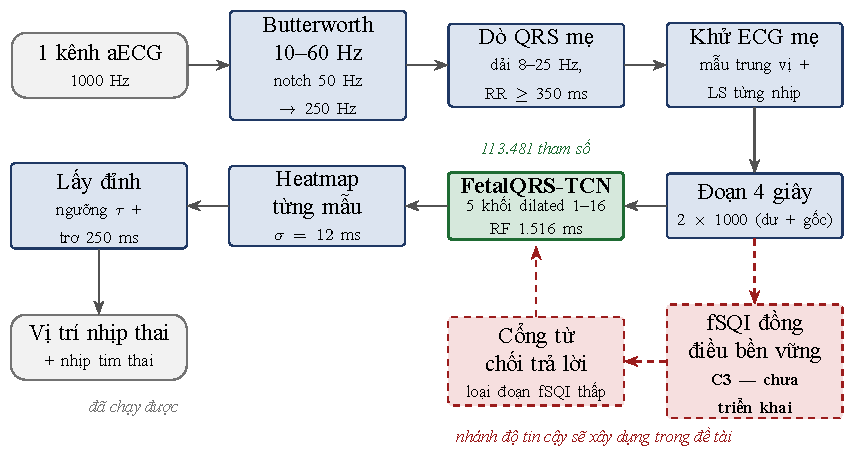
\includegraphics[width=\textwidth]{figs/fig0_pipeline.pdf}
\caption{Pipeline \hethong{}. Khối màu xanh lá là mạng học sâu. Các khối viền đỏ nét đứt là nhánh độ
tin cậy (đóng góp C3). Prototype của nhánh này đã chạy: phần \textit{cổng từ chối} có tác dụng và đã
vào demo; phần \textit{đồng điều bền vững} cho kết quả phủ định và được rút lại (\S\ref{sec:fsqi}).}
\label{fig:pipeline}
\end{figure}

\subsection{Mô hình: \mh{}}

\begin{table}[H]\centering\small
\caption{Đặc tả \mh{}. Mọi con số đều đo trực tiếp từ mã nguồn và checkpoint, không lấy lại từ tài liệu.}
\label{tab:mohinh}
\begin{tabular}{@{}L{5.0cm} L{9.4cm}@{}}
\toprule
\textbf{Thuộc tính} & \textbf{Giá trị} \\
\midrule
Tiền xử lý & Butterworth 10--60\,Hz pha không (zero-phase) + chặn dải 50\,Hz ($Q=30$), hạ tần số về 250\,Hz \\
Khử ECG mẹ & Dò QRS mẹ ở dải 8--25\,Hz với RR tối thiểu 350\,ms; mẫu trung vị cửa sổ $[-150, +300]$\,ms;
trừ theo hệ số bình phương tối thiểu riêng cho từng nhịp \\
Đầu vào mạng & $2 \times 1000$: tín hiệu dư sau khử mẹ và tín hiệu gốc, đoạn 4 giây ở 250\,Hz \\
Thân mạng & Conv1d($k=7$) + 5 khối dư giãn nở với hệ số $1, 2, 4, 8, 16$ \\
Trường tiếp nhận & 379 mẫu $=$ \textbf{1.516\,ms} \\
Đầu ra & Một logit cho \textbf{từng mẫu}; nhãn là bản đồ nhiệt Gauss $\sigma = 12$\,ms \\
Hậu xử lý & Lấy đỉnh với ngưỡng $\tau$ và thời gian trơ 250\,ms \\
\midrule
Tham số huấn luyện được & \textbf{113.481} \\
Kích thước checkpoint & 0,48 MB \\
Độ trễ một cửa sổ 4 giây & \textbf{4,35\,ms} trên CPU (hệ số thời gian thực 920$\times$) \\
\bottomrule
\end{tabular}
\end{table}

\subsection{Vì sao chọn mô hình này, và vì sao đây không phải bắt chước}

Câu hỏi này quan trọng vì trong nhóm có một thành viên khác đang làm hướng Persistence Image kết hợp
CNN hai nhánh. Nhóm khẳng định lựa chọn của mình đến từ thực nghiệm, và trên thực tế nó \textbf{bác bỏ}
chính giả thuyết trung tâm của hướng kia.

\begin{table}[H]\centering\small
\caption{Đối chiếu hai hướng tiếp cận trên từng trục thiết kế.}
\label{tab:doichieu}
\begin{tabular}{@{}L{3.6cm} L{5.3cm} L{5.5cm}@{}}
\toprule
\textbf{Trục thiết kế} & \textbf{Hướng Persistence Image} & \textbf{\mh{} (nhóm)} \\
\midrule
Biểu diễn đầu vào & Ảnh bền vững 2 chiều từ nhúng trễ & Tín hiệu 1 chiều thô + tín hiệu dư \\
Dạng bài toán & Phân loại cửa sổ có/không có QRS & Hồi quy bản đồ nhiệt theo từng mẫu \\
Dải thông & 1--45\,Hz & \textbf{10--60\,Hz} \\
Ngữ cảnh thời gian & 300\,ms & \textbf{4 giây}, trường tiếp nhận 1.516\,ms \\
Vai trò của topo & Đặc trưng chính để dò đỉnh & Chỉ số chất lượng, quyền từ chối (C3) \\
Tham số & 1.522.476 (đo thật trong mã nguồn) & \textbf{113.481} \\
\bottomrule
\end{tabular}
\end{table}

Ba thí nghiệm có kiểm soát dưới đây là cơ sở của lựa chọn.

\paragraph{Thí nghiệm 1 --- so 16 kiến trúc ở cùng ngân sách tham số.}
\begin{figure}[H]\centering
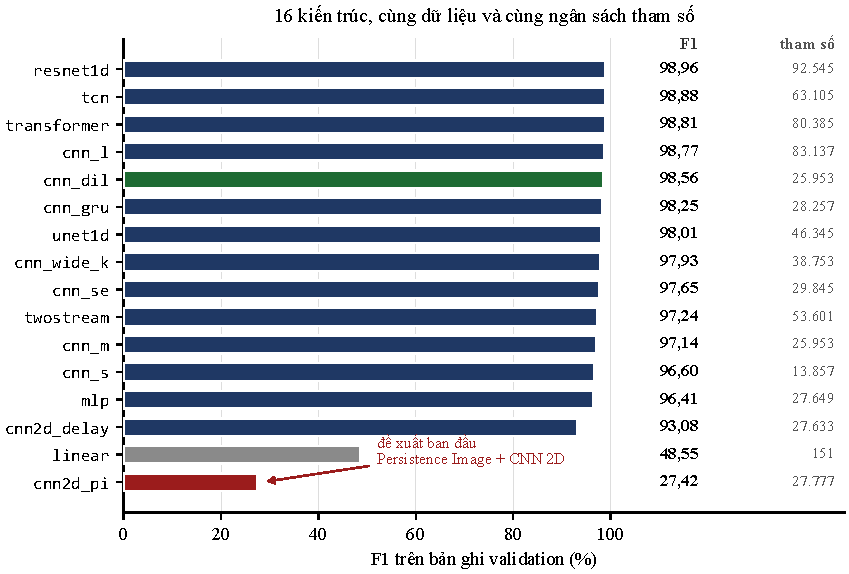
\includegraphics[width=0.96\textwidth]{figs/fig3_kien_truc.pdf}
\caption{Mười sáu kiến trúc, cùng dữ liệu và cùng ngân sách tham số. Persistence Image kết hợp CNN 2D
đứng cuối bảng.}
\label{fig:arch}
\end{figure}

\begin{canhbao}[title={Bảng \ref{fig:arch} là bảng cũ và lạc quan --- giữ lại để minh bạch}]
Bảng đó chạy ở dải 3--90\,Hz, trên một bản ghi validation, một seed, và F1 là giá trị lớn nhất quét trên
18 ngưỡng ngay trên bản ghi đánh giá. Nhóm đã \textbf{chạy lại} với giao thức đúng; kết quả ở ngay dưới.
Bảng cũ chỉ còn giá trị ở một điểm: Persistence Image thua ở mức không thể cứu (27,42), và điều đó không
đổi dưới bất kỳ giao thức nào.
\end{canhbao}

\paragraph{Bảng kiến trúc chạy lại đúng giao thức.} Dải 10--60\,Hz, tách theo bản ghi 5 fold, ngưỡng chọn
\textbf{trên bản ghi validation riêng} rồi áp cố định sang bản ghi test, 20 đánh giá (bản ghi $\times$ kênh),
Wilcoxon ghép cặp so với \texttt{cnn\_dil}. Cửa sổ 300\,ms như bảng cũ, để so được với nó. Mã tại
\texttt{pilot\_evidence/arch\_loro.py}.

\begin{figure}[H]\centering
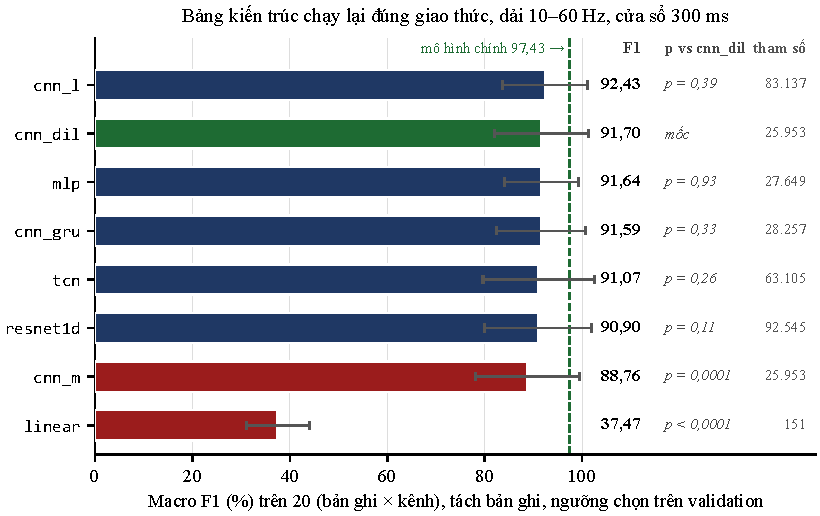
\includegraphics[width=0.96\textwidth]{figs/fig13_kien_truc_v2.pdf}
\caption{Tám kiến trúc dưới giao thức trung thực. Sáu kiến trúc nằm trong 1,5 điểm nhau và \textbf{không
kiến trúc nào khác \texttt{cnn\_dil} có ý nghĩa thống kê}. Đường đứt xanh là mô hình chính (ngữ cảnh 4 giây,
đầu ra từng mẫu) --- cách xa cả nhóm.}
\label{fig:arch_v2}
\end{figure}

\begin{table}[H]\centering\small
\caption{Số liệu của hình \ref{fig:arch_v2}. Một seed, ba epoch (loss vẫn đang giảm ở epoch cuối, nên
mọi con số đều còn dư địa nhưng \textit{cùng} dư địa).}
\label{tab:arch_v2}
\begin{tabular}{@{}C{0.9cm} L{2.2cm} R{1.8cm} C{2.6cm} C{1.9cm} C{2.2cm} C{1.5cm}@{}}
\toprule
\textbf{Hạng} & \textbf{Kiến trúc} & \textbf{Tham số} & \textbf{Macro F1} & \textbf{Hiệu số} &
\textbf{$p$ Wilcoxon} & \textbf{Hạng cũ} \\
\midrule
1 & \texttt{cnn\_l} & 83.137 & $92{,}43 \pm 8{,}73$ & $+0{,}73$ & 0,388 & 4 \\
2 & \texttt{cnn\_dil} & 25.953 & $91{,}70 \pm 9{,}68$ & mốc & --- & 5 \\
3 & \texttt{mlp} & 27.649 & $91{,}64 \pm 7{,}64$ & $-0{,}07$ & 0,927 & 13 \\
4 & \texttt{cnn\_gru} & 28.257 & $91{,}59 \pm 9{,}10$ & $-0{,}12$ & 0,330 & 6 \\
5 & \texttt{tcn} & 63.105 & $91{,}07 \pm 11{,}41$ & $-0{,}64$ & 0,260 & 2 \\
6 & \texttt{resnet1d} & 92.545 & $90{,}90 \pm 10{,}98$ & $-0{,}81$ & 0,105 & 1 \\
7 & \texttt{cnn\_m} & 25.953 & $88{,}76 \pm 10{,}61$ & $-2{,}95$ & \textbf{0,0001} & 11 \\
8 & \texttt{linear} & 151 & $37{,}47 \pm 6{,}47$ & $-54{,}24$ & \textbf{$<$0,0001} & 15 \\
\bottomrule
\end{tabular}
\end{table}

Ba điều bảng này nói, rõ hơn bảng cũ rất nhiều:

\begin{enumerate}[leftmargin=1.6em,itemsep=3pt]
\item \textbf{Họ kiến trúc không quan trọng.} Mạng dư 92 nghìn tham số, TCN 63 nghìn, GRU, và cả một MLP
27 nghìn tham số đều không phân biệt được với CNN giãn nở 26 nghìn tham số. Quán quân cũ
(\texttt{resnet1d}) rơi xuống hạng 6.
\item \textbf{Giãn nở có quan trọng.} \texttt{cnn\_m} và \texttt{cnn\_dil} có \textit{cùng} 25.953 tham số,
chỉ khác lịch giãn nở, chênh 2,95 điểm với $p = 0{,}0001$. Đây là bằng chứng có kiểm soát chặt nhất trong
đề tài rằng trường tiếp nhận là biến chi phối.
\item \textbf{Cả tám đều thua xa mô hình chính.} Tốt nhất trong bảng là 92,43; mô hình 4 giây đầu ra từng
mẫu đạt 97,43 trên cùng giao thức. Chênh 5 điểm đến từ ngữ cảnh và độ phân giải đầu ra, không từ họ mạng.
\end{enumerate}

\paragraph{Thí nghiệm 2 --- quét trường tiếp nhận.}
Đây mới là biến kiến trúc thực sự quan trọng. Cùng một họ mạng, chỉ đổi lịch giãn nở:

\begin{figure}[H]\centering
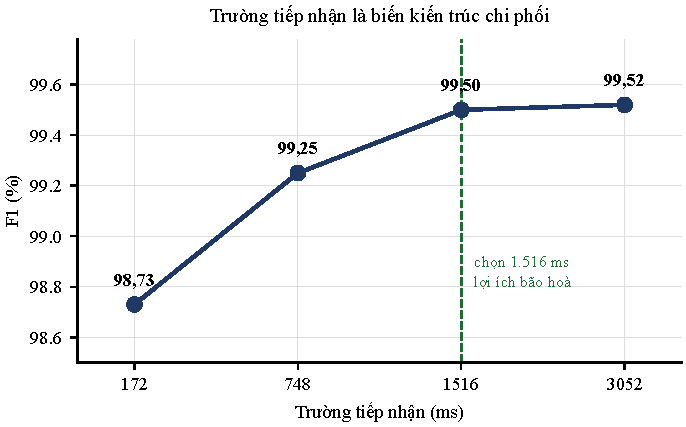
\includegraphics[width=0.78\textwidth]{figs/fig4_truong_tiep_nhan.pdf}
\caption{Lợi ích của trường tiếp nhận bão hoà quanh 1,5 giây. Nhóm chọn 1.516\,ms.}
\label{fig:rf}
\end{figure}

Kiểm chứng bằng ba seed với giao thức tách theo bản ghi đầy đủ: trường tiếp nhận 1.516\,ms đạt
$97{,}16 \pm 4{,}34$, trường 172\,ms đạt $92{,}67 \pm 10{,}46$. Wilcoxon ghép cặp cho
$p = 0{,}0000$. Chênh lệch 4,66 điểm, và độ lệch chuẩn giảm hơn một nửa --- ngữ cảnh dài làm mô hình
ổn định hơn giữa các sản phụ.

\paragraph{Thí nghiệm 3 --- đầu ra theo từng mẫu.}
Chuyển từ phân loại cửa sổ sang hồi quy bản đồ nhiệt theo từng mẫu cải thiện độ chính xác định vị đỉnh
từ 5,6--6,0\,ms xuống \textbf{1,0\,ms}. Đây là điều kiện bắt buộc nếu muốn so với các công trình dùng
dung sai chặt hơn 50\,ms, và là tiền đề cho phân tích biến thiên nhịp tim thai.

\begin{ghichu}[title={Kết luận về lựa chọn mô hình}]
Nhóm chọn mạng tích chập giãn nở dạng chuỗi sang chuỗi \textbf{không phải vì họ kiến trúc này ưu việt},
mà vì nó là cách \textbf{rẻ nhất} để mua hai thứ mà thực nghiệm chỉ ra là thật sự quan trọng:
trường tiếp nhận dài khoảng 1,5 giây, và độ phân giải đầu ra theo từng mẫu.

Bằng chứng: ở cùng trường tiếp nhận khoảng 1,5 giây, U-Net 1 chiều tốn 678.257 tham số mà F1 lại thấp
hơn (99,42 so với 99,50); Transformer chậm gấp 21,7 lần để đổi lấy 0,25 điểm.
\end{ghichu}

\clearpage

% ================================================================= 5. KẾT QUẢ TIỀN KHẢ THI
\section{Kết quả tiền khả thi đã đo}
\label{sec:ketqua}

Mọi con số trong mục này do nhóm tự đo, có mã nguồn và nhật ký kèm theo trong thư mục
\texttt{pilot\_evidence/}, \texttt{model/} và \texttt{benchmark\_dpss/}.

\subsection{Thiết lập}

Dữ liệu: PhysioNet ADFECGDB, 5 sản phụ $\times$ 4 kênh bụng, 1000\,Hz, nhãn chuẩn từ điện cực xoắn da đầu
thai đã được bác sĩ tim mạch duyệt. Toàn bộ tệp tải trực tiếp từ PhysioNet bằng
\texttt{model/download\_data.py} và được ghi mã băm SHA-256 trong \texttt{data\_card.json}.
Giao thức: tách theo bản ghi, ngưỡng quyết định chọn trên \textbf{một bản ghi validation riêng},
chấm điểm ở mức sự kiện với dung sai $\pm$50\,ms. Tổng khối lượng: trên 600.000 cửa sổ, khoảng sáu giờ
tính toán trên CPU.

\subsection{Phân rã đóng góp ba tầng}

\begin{figure}[H]\centering
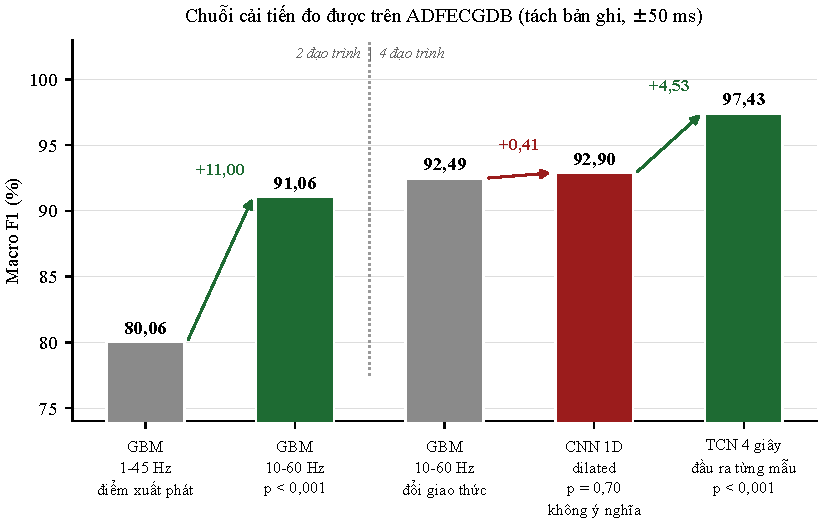
\includegraphics[width=0.92\textwidth]{figs/fig1_chuoi_cai_tien.pdf}
\caption{Chuỗi cải tiến đo được. Bước có ý nghĩa thống kê tô xanh, bước không có ý nghĩa tô đỏ.
Đường chấm đánh dấu chỗ \textbf{đổi giao thức} từ 2 sang 4 đạo trình --- hai bên đường này không
trừ trực tiếp cho nhau được, nên mức tăng $+11{,}00$ chỉ tính trong phần bên trái.}
\label{fig:waterfall}
\end{figure}

\begin{canhbao}[title={Nhóm tự sửa một phát biểu sai của bản đề cương trước}]
Bản trước ghi ``đổi dải lọc ăn +12,43 điểm''. Con số đó \textbf{sai}, vì nó trộn hai thí nghiệm khác
nhau: 80,06 đo trên \textbf{2} đạo trình trong khảo sát dải, còn 92,49 đo trên \textbf{4} đạo trình
trong thí nghiệm cuối. Con số có kiểm soát nội bộ đúng là \tot{+11,00} (91,06 so với 80,06, cùng một
thí nghiệm, cùng số đạo trình).

Bản trước cũng phát biểu ``tiền xử lý quan trọng gấp 30 lần kiến trúc''. Phát biểu đó \textbf{không đứng
vững}, vì bước ``+4,53 điểm'' được gán nhãn tiền xử lý thực ra gộp ba thay đổi, trong đó có hai thay đổi
mang bản chất kiến trúc: trường tiếp nhận và tham số hoá đầu ra. Phát biểu đúng là \textbf{phân rã ba tầng}
ở bảng \ref{tab:phanra}.
\end{canhbao}

\begin{figure}[H]\centering
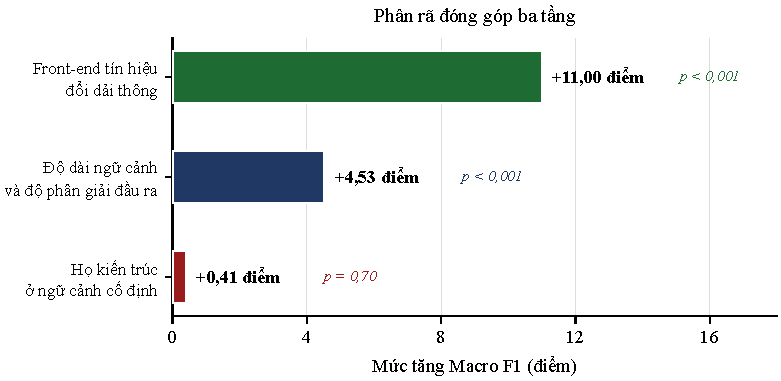
\includegraphics[width=0.8\textwidth]{figs/fig7_dong_gop.pdf}
\caption{Phân rã đóng góp ba tầng. Front-end tín hiệu vẫn là tầng lớn nhất, nhưng khoảng cách so với
tầng ngữ cảnh là 2,4 lần chứ không phải 30 lần như bản đề cương trước phát biểu.}
\label{fig:dongop}
\end{figure}

\begin{table}[H]\centering\small
\caption{Phân rã đóng góp ba tầng. Đây là phát biểu nhóm sẽ dùng trong bài báo.}
\label{tab:phanra}
\begin{tabular}{@{}L{6.4cm} C{2.6cm} C{2.4cm} L{2.4cm}@{}}
\toprule
\textbf{Tầng} & \textbf{Mức tăng F1} & \textbf{Trị số \textit{p}} & \textbf{Kết luận} \\
\midrule
Front-end tín hiệu (đổi dải thông) & \tot{+11,00} & $< 0{,}001$ & có ý nghĩa \\
Độ dài ngữ cảnh và độ phân giải đầu ra & \tot{+4,53} & $0{,}0000$ & có ý nghĩa \\
Họ kiến trúc, ở ngữ cảnh cố định & \xau{+0,41} & $0{,}7012$ & \xau{không có ý nghĩa} \\
\bottomrule
\end{tabular}
\end{table}

\begin{figure}[H]\centering
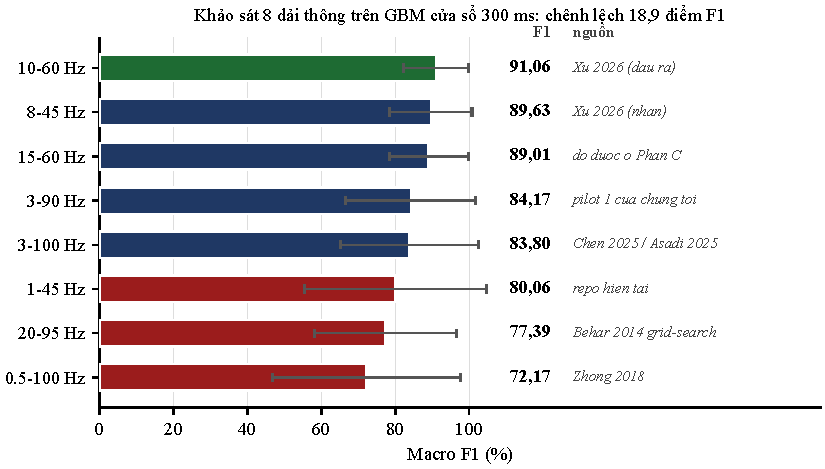
\includegraphics[width=0.94\textwidth]{figs/fig2_dai_loc.pdf}
\caption{Khảo sát tám dải thông, mỗi dải là một lần chạy tách theo bản ghi đầy đủ. Chênh lệch giữa dải
tốt nhất và kém nhất là 18,89 điểm F1 --- lớn hơn toàn bộ khác biệt giữa 16 kiến trúc học sâu.}
\label{fig:band}
\end{figure}

Ba nguồn y văn độc lập đọc từ toàn văn ủng hộ hướng này: Behar và cộng sự 2014 tìm kiếm lưới ra
20--95\,Hz; Clifford và cộng sự 2014 ghi nhận cắt thông cao ở 10\,Hz cải thiện kết quả do loại bỏ sóng P
và T của mẹ; Xu và cộng sự 2026 dùng đúng 10--60\,Hz.

Một chi tiết nhóm muốn nêu vì nó phản trực giác: dải có \textbf{tương phản cao nhất} (20--95\,Hz, tỉ số
RMS 1,94) lại cho F1 gần \textbf{thấp nhất} (77,39). Tương phản không phải hàm mục tiêu.

\subsection{Quy tắc chọn kênh mù nhãn}
\label{sec:chonkenh}

Đây là kết quả nhóm coi là quan trọng nhất trong đợt thực nghiệm vừa rồi, và nó xuất phát từ một
lỗi liêm chính mà nhóm tự phát hiện.

\begin{canhbao}[title={Lỗi nhóm tự phát hiện và đã sửa}]
Con số ``77,52'' mà bản đề cương trước báo cáo cho thí nghiệm xuyên bộ dữ liệu là kết quả
\textbf{chọn kênh tốt nhất bằng nhãn thật}. Đó là chọn kênh kiểu ``thần thánh'' (oracle), không dùng
được trong thực tế và không được phép báo cáo như hiệu năng hệ thống.
\end{canhbao}

Nhóm đã thay bằng quy tắc chọn kênh \textbf{mù nhãn} theo Power-MF: chọn kênh có đỉnh mật độ phổ công
suất lớn nhất trong dải nhịp tim thai 1,8--3,0\,Hz (tương ứng 108--180 nhịp/phút), tính trên đường bao
năng lượng của tín hiệu dư. Quy tắc này không dùng nhãn và có thể đăng ký trước.

\begin{table}[H]\centering\small
\caption{So sánh bốn quy tắc chọn kênh. Quy tắc mù nhãn đạt \textbf{đúng bằng} oracle trong miền,
nhưng \textbf{sụp đổ} ngoài miền.}
\label{tab:chonkenh}
\begin{tabular}{@{}L{6.0cm} C{3.4cm} C{3.4cm}@{}}
\toprule
\textbf{Quy tắc chọn kênh} & \textbf{ADFECGDB (trong miền)} & \textbf{CinC 2013 (ngoài miền)} \\
\midrule
Mù nhãn theo mật độ phổ công suất & \tot{99,21} & \xau{59,15} \\
Kênh cố định (kênh đầu tiên) & 98,09 & \tot{77,34} \\
Bản đồ đạo trình do giao thức quy định & 99,18 & --- \\
Oracle, dùng nhãn thật & \textit{99,21} & \textit{77,59} \\
Trung bình trên cả 4 kênh & 97,45 & 61,96 \\
\bottomrule
\end{tabular}
\end{table}

\begin{ghichu}[title={Phát hiện khoa học và ý nghĩa của nó}]
Quy tắc chọn kênh mù nhãn đạt \textbf{đúng bằng oracle} khi ở trong miền (99,21 so với 99,21), nhưng
\textbf{sụp đổ hoàn toàn} khi ra ngoài miền (59,15 so với 77,34 của một quy tắc cố định đơn giản hơn).

Nói cách khác: một chỉ số chất lượng dựa trên phổ hoạt động tốt đúng ở nơi ta không cần nó, và hỏng
đúng ở nơi ta cần. \textbf{Đây là động cơ trực tiếp và đã đo được cho đóng góp C3} --- cần một chỉ số
chất lượng học được hoặc dựa trên cấu trúc topo, chứ không phải một heuristic phổ.
\end{ghichu}

\subsection{Kết quả cuối trên ADFECGDB}

\begin{table}[H]\centering\small
\caption{Hiệu năng \mh{}, tách theo bản ghi, dung sai $\pm$50\,ms. Mỗi bản ghi được chấm bằng
checkpoint chưa từng nhìn thấy bản ghi đó.}
\label{tab:ketqua}
\begin{tabular}{@{}L{6.2cm} C{2.1cm} C{1.9cm} C{1.9cm} C{2.0cm}@{}}
\toprule
\textbf{Giao thức} & \textbf{Macro F1} & \textbf{Se} & \textbf{PPV} & \textbf{Jitter} \\
\midrule
Kênh chọn mù nhãn (báo cáo chính) & \tot{99,21} & 99,59 & 98,79 & 3,05\,ms \\
Trung bình trên cả 4 kênh & 97,45 & 97,69 & 97,18 & 3,62\,ms \\
Ba seed, cả 4 kênh & $97{,}16 \pm 4{,}34$ & 97,05 & 97,28 & 3,64\,ms \\
\midrule
Gộp toàn cục (micro) & 99,17 & \multicolumn{3}{l}{TP 3.178 \quad FP 40 \quad FN 13 \quad trên 3.191 nhịp} \\
\bottomrule
\end{tabular}
\end{table}

\subsection{Nơi hệ thống sụp đổ}

\begin{figure}[H]\centering
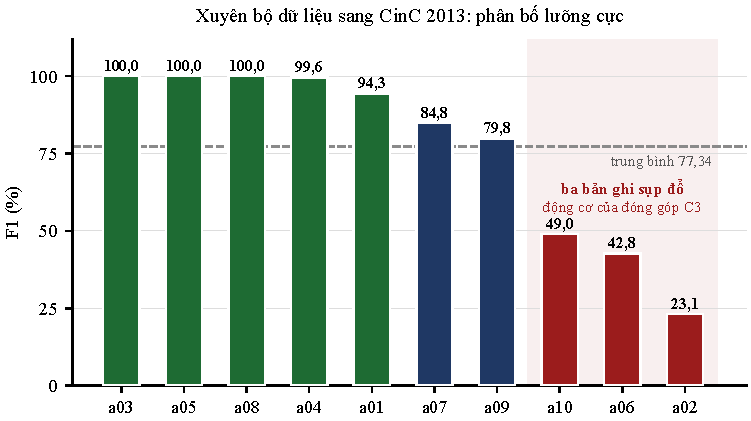
\includegraphics[width=0.94\textwidth]{figs/fig6_luong_cuc.pdf}
\caption{Chuyển sang PhysioNet/CinC 2013 mà không tinh chỉnh. Phân bố \textbf{lưỡng cực}: bốn bản ghi
hoàn hảo, ba bản ghi sụp dưới 50\%. Chính hình dạng này, chứ không phải con số trung bình, là vấn đề
cần giải.}
\label{fig:bimodal}
\end{figure}

Một hệ thống theo dõi thai mà im lặng đưa ra nhịp tim với độ chính xác 23\% thì nguy hiểm hơn một hệ
thống nói ``tôi không đọc được tín hiệu này''. Đó chính là lý do C3 tồn tại.

% ================================================================= BASELINE TỰ CÀI LẠI
\subsection{Baseline cổ điển tự cài lại}
\label{sec:baselines}

Bản đề cương trước thừa nhận một điểm yếu: mọi so sánh với y văn đều là so với \textit{con số đã công
bố}, không phải với bản tự chạy. Nhóm đã khắc phục. Ba baseline không dùng học máy được cài lại từ đầu
trong \texttt{baselines/ts\_baseline.py} và chấm trên \textbf{cùng dữ liệu, cùng giao thức, cùng hàm khớp
nhịp} với mô hình của nhóm.

\begin{table}[H]\centering\small
\caption{Ba baseline cổ điển. Siêu tham số của mỗi baseline được chọn \textbf{chỉ trên r01} rồi áp
nguyên cho bốn bản ghi còn lại; cột ``16 giữ lại'' loại r01 khỏi phép tính.}
\label{tab:baseline_mota}
\begin{tabular}{@{}L{2.6cm} L{6.2cm} L{5.6cm}@{}}
\toprule
\textbf{Baseline} & \textbf{Khử ECG mẹ} & \textbf{Dò QRS thai} \\
\midrule
TS & Mẫu trung bình, trừ trực tiếp & Pan--Tompkins thích nghi, trơ 250\,ms \\
TS-PCA & Mẫu từ 2 thành phần chính của các nhịp mẹ (theo Behar 2014) & Pan--Tompkins thích nghi \\
Prominence & \textbf{Đúng front-end của nhóm}: mẫu trung vị + bình phương tối thiểu từng nhịp &
\texttt{find\_peaks}, độ nhô $\geq$ trung vị $+ 3\,$MAD, cách nhau $\geq$ 250\,ms \\
\bottomrule
\end{tabular}
\end{table}

Baseline thứ ba là quan trọng nhất về mặt khoa học: nó dùng \textbf{cùng tín hiệu dư} mà mạng nhận vào,
chỉ thay mạng bằng phép lấy đỉnh đơn giản. Hiệu số giữa nó và mô hình đo \textbf{đúng phần đóng góp của
mạng nơ-ron}, tách khỏi phần đóng góp của tiền xử lý.

\begin{table}[H]\centering\small
\caption{Kết quả trên ADFECGDB, dung sai $\pm$50\,ms. Hiệu số và khoảng tin cậy tính ở \textbf{mức chủ
thể} ($n = 5$ sản phụ, trung bình 4 kênh trước). Các trị số $p$ của bản 3.2 tính trên 20 cặp (bản ghi
$\times$ kênh) là \textbf{giả lập} và đã bị gỡ --- xem \S\ref{sec:thongke}.}
\label{tab:baseline_kq}
\begin{tabular}{@{}L{2.4cm} C{2.2cm} C{1.4cm} C{1.6cm} C{1.4cm} C{2.4cm} C{2.4cm}@{}}
\toprule
\textbf{Phương pháp} & \textbf{4 kênh (20)} & \textbf{16 giữ lại} & \textbf{Kênh PSD} &
\textbf{Hiệu số} & \textbf{KTC 95\% bootstrap} & \textbf{KTC 95\% $t$} \\
\midrule
TS + PT & $78{,}96 \pm 23{,}52$ & 75,55 & 87,68 & $-18{,}49$ & $[-30{,}60; -6{,}38]$ &
\xau{$[-38{,}80; +1{,}81]$} \\
TS-PCA + PT & $91{,}05 \pm 10{,}17$ & 90,94 & 96,74 & $-6{,}40$ & $[-8{,}09; -4{,}70]$ &
\tot{$[-9{,}10; -3{,}69]$} \\
Prominence & $86{,}39 \pm 11{,}14$ & 84,99 & 92,03 & $-11{,}06$ & $[-14{,}51; -7{,}80]$ &
\tot{$[-16{,}38; -5{,}73]$} \\
\midrule
\textbf{\mh{}} & $\mathbf{97{,}45 \pm 4{,}44}$ & \textbf{96,81} & \textbf{99,21} & --- & --- & --- \\
\bottomrule
\end{tabular}
\end{table}

\begin{canhbao}[title={Ba baseline này KHÔNG cùng độ chắc --- bản 3.2 trình bày chúng như nhau}]
Với \textbf{TS-PCA} và \textbf{Prominence}, KTC 95\% của hiệu số loại trừ 0 ở \textbf{cả} bootstrap lẫn
thang $t$ --- hướng kết quả vững, chỉ là không được tuyên bố ý nghĩa thống kê từ 5 phụ nữ.

Với \textbf{TS} thì khác: KTC 95\% kiểu $t$ là $[-38{,}80;\ +1{,}81]$ --- \textbf{chứa 0}. Hiệu số
18,49 điểm hoàn toàn do biến thiên giữa 5 bản ghi, không phải một lợi thế ổn định. Đây là baseline yếu
nhất về mặt bằng chứng, dù trông là baseline nhóm thắng đậm nhất.
\end{canhbao}

Ba điều rút ra, xếp theo mức quan trọng:

\begin{enumerate}[leftmargin=1.6em,itemsep=4pt]
\item \textbf{Mạng nơ-ron đáng $+11{,}06$ điểm} so với lấy đỉnh trên cùng tín hiệu dư, KTC 95\% kiểu $t$
$[+5{,}73;\ +16{,}38]$ loại trừ 0. Đây là con số trả lời câu hỏi ``mạng có thật sự cần không'' --- và câu
trả lời là có, nhưng chỉ khi front-end đã đúng.
\item \textbf{TS-PCA là baseline cổ điển mạnh.} Trên kênh chọn mù nhãn nó đạt 96,74, chỉ kém mô hình
2,47 điểm. Điều này nhất quán với Power-MF (98,0 bằng phương pháp cổ điển) và củng cố luận điểm chính:
phần lớn hiệu năng nằm ở front-end, không ở mạng.
\item \textbf{Độ lệch chuẩn giảm hơn một nửa} (4,44 so với 10,17 của baseline tốt nhất). Mạng không chỉ
cao hơn trung bình mà còn \textit{ổn định hơn} giữa các sản phụ và kênh.
\end{enumerate}

\begin{ghichu}[title={Power-MF: bản 3.2 nói không chạy lại được --- bản 3.4 đã chạy, ở hai cấu hình}]
Bản 3.2 ghi rằng Power-MF cần MATLAB R2021a và các hàm ICA đa kênh của Varanini 2014 không có trong kho
mã công bố, nên không chạy lại được. \textbf{Phát biểu đó đã bị rút.} Power-MF chạy được trên
\textbf{GNU Octave 11.3.0} sau bảy bản vá, và được chấm bằng \textbf{chính bộ chấm của nhóm} trên
\textbf{cả 22 chủ thể}. Con số công bố cho Silesia B1 là 99,46; nhóm chạy lại được \textbf{99,40} ---
lệch 0,06 điểm.

Nhóm cài thêm \textbf{Power-MF-1ch}: cùng thuật toán, cùng front-end và bộ khử mẹ của nhóm, nhưng chỉ
\textbf{một đạo trình}. Đây là đối chứng công bằng nhất trong cả đề cương, vì mọi thứ trừ thuật toán lõi
đều giống hệt nhau. Nó đạt 86,71 --- kém \hethong{} 10,85 điểm, thua 22/22 chủ thể.

\xau{Cảnh báo:} mọi con số Power-MF của bản 3.3 (94,87 / 98,38 / 97,33 / hiệu số $+2{,}74$ và $-1{,}06$)
đứng trên một bản Octave hỏng vì lỗi cổng chuyển của nhóm, và \textbf{đã bị rút toàn bộ}. Xem hộp đầu
\S\ref{sec:powermf}.
\end{ghichu}


% ================================================================= MỞ RỘNG SANG SILESIA
\subsection{Mở rộng sang 22 sản phụ và sang thai kỳ}
\label{sec:silesia}

Điểm yếu lớn nhất của bản đề cương trước là chỉ có 5 sản phụ, tất cả đang chuyển dạ. Nhóm đã tải bộ
Silesia (Matonia và cộng sự, \textit{Scientific Data} 7:200, 2020; figshare DOI 10.6084/m9.figshare.c.4740794,
giấy phép CC0), gồm \textbf{10 sản phụ thai kỳ 32--42 tuần} (B1, mỗi người 20 phút) và \textbf{12 sản phụ chuyển
dạ} (B2, mỗi người 5 phút), cùng bệnh viện và cùng hệ ghi KOMPOREL với dữ liệu huấn luyện. Toàn bộ do
\texttt{model/download\_silesia.py} tải với mã băm SHA-256 ghi lại.

\subsubsection{Kiểm tra rò rỉ trước khi đánh giá}

Bài báo gốc tự khai rằng 5 bản ghi PhysioNet được lấy từ bộ chuyển dạ. Nhóm không tin lời khai mà đo lại
bằng tín hiệu: đưa cả hai về 250\,Hz, trượt cửa sổ 60 giây của từng bản ghi PhysioNet trên toàn bộ từng
bản ghi B2, thử mọi tổ hợp 4$\times$4 đạo trình và mọi độ lệch $\pm$5 phút.

\begin{table}[H]\centering\small
\caption{Kết quả kiểm tra rò rỉ. NCC là tương quan chéo chuẩn hoá cực đại. Cột ``hạng nhì'' là NCC với
bản ghi B2 gần nhất còn lại, để thấy khoảng cách.}
\label{tab:roriSilesia}
\begin{tabular}{@{}C{1.6cm} C{1.6cm} C{1.6cm} C{2.0cm} C{1.8cm} C{2.2cm} C{2.2cm}@{}}
\toprule
\textbf{PhysioNet} & \textbf{Silesia} & \textbf{NCC} & \textbf{Lệch} & \textbf{Hạng nhì} &
\textbf{Nhãn khớp} & \textbf{Số nhịp} \\
\midrule
r01 & B2\_01 & 0,989 & $-56$\,ms & 0,135 & 100,0\% & 644 / 644 \\
r10 & B2\_02 & 0,993 & $-40$\,ms & 0,147 & 99,8\% & 637 / 637 \\
r04 & B2\_07 & 0,994 & $-48$\,ms & 0,178 & 99,8\% & 632 / 632 \\
r07 & B2\_10 & 0,994 & $-48$\,ms & 0,141 & 99,8\% & 627 / 627 \\
r08 & B2\_11 & 0,988 & $-56$\,ms & 0,128 & 98,8\% & 651 / 646 \\
\bottomrule
\end{tabular}
\end{table}

Kết luận: 5/12 bản ghi B2 \textbf{chính là} 5 bản ghi PhysioNet. Hệ quả thứ nhất: số sản phụ độc lập
là \textbf{22}, không phải 27. Hệ quả thứ hai: với 5 bản ghi trùng, nhóm dùng checkpoint fold tương ứng
(chưa từng thấy bản ghi đó); 7 bản ghi B2 còn lại và 10 bản ghi B1 dùng checkpoint production, zero-shot.

\subsubsection{Kết quả}

\begin{table}[H]\centering\small
\caption{Cùng một mô hình, cùng giao thức $\pm$50\,ms, trên năm cấu hình dữ liệu. ``$\geq$90'' và ``$<$50''
là số bản ghi có F1 (kênh PSD) trong khoảng đó.}
\label{tab:silesia_tonghop}
\begin{tabular}{@{}L{5.0cm} C{0.8cm} C{1.2cm} C{2.6cm} C{2.6cm} C{0.8cm} C{0.8cm}@{}}
\toprule
\textbf{Bộ dữ liệu} & $n$ & \textbf{Phút} & \textbf{F1, kênh PSD} & \textbf{F1, 4 kênh} & $\geq$90 & $<$50 \\
\midrule
ADFECGDB PhysioNet, tách bản ghi & 5 & 25 & $99{,}21 \pm 1{,}50$ & $97{,}45 \pm 2{,}96$ & 5 & 0 \\
Silesia B2 chuyển dạ, 12 bản ghi & 12 & 60 & $97{,}17 \pm 7{,}45$ & $95{,}26 \pm 9{,}59$ & 11 & 0 \\
\quad chỉ 7 bản ghi hoàn toàn mới, zero-shot & 7 & 35 & $95{,}87 \pm 9{,}75$ & $93{,}73 \pm 12{,}48$ & 6 & 0 \\
\textbf{Silesia B1 thai kỳ 32--42 tuần, zero-shot} & 10 & 199,6 & $\mathbf{93{,}30 \pm 13{,}46}$ &
$\mathbf{91{,}31 \pm 9{,}99}$ & 8 & 0 \\
CinC 2013 set-a, zero-shot & 10 & 10 & $59{,}15 \pm 37{,}17$ & $61{,}96 \pm 34{,}09$ & 4 & 5 \\
\bottomrule
\end{tabular}
\end{table}

\begin{table}[H]\centering\small
\caption{Silesia B1 --- thai kỳ, từng bản ghi. Mô hình chưa từng thấy bất kỳ dữ liệu thai kỳ nào.
Cột ``oracle'' là kênh tốt nhất theo nhãn, chỉ để tham chiếu.}
\label{tab:silesiaB1}
\begin{tabular}{@{}C{1.3cm} C{1.3cm} C{1.5cm} C{1.4cm} C{1.4cm} C{1.6cm} C{1.6cm} C{1.5cm}@{}}
\toprule
\textbf{Bản ghi} & \textbf{Kênh PSD} & \textbf{F1 PSD} & \textbf{Se} & \textbf{PPV} & \textbf{Jitter} &
\textbf{F1 4 kênh} & \textbf{Oracle} \\
\midrule
B1\_01 & A3 & 97,70 & 96,70 & 98,72 & 10,3\,ms & 87,79 & 97,70 \\
B1\_02 & A3 & 99,59 & 99,50 & 99,68 & 9,1\,ms & 97,97 & 99,59 \\
B1\_03 & A3 & 99,86 & 99,88 & 99,84 & 2,5\,ms & 99,17 & 99,86 \\
B1\_04 & A3 & 99,80 & 99,64 & 99,96 & 3,8\,ms & 98,59 & 99,96 \\
B1\_05 & A3 & 99,78 & 99,75 & 99,82 & 3,6\,ms & 99,47 & 99,78 \\
B1\_06 & A4 & 80,90 & 78,05 & 83,95 & 12,5\,ms & 92,43 & 98,28 \\
B1\_07 & A4 & \xau{58,72} & 53,21 & 65,49 & 15,3\,ms & 67,96 & 78,52 \\
B1\_08 & A1 & 99,52 & 99,28 & 99,76 & 7,3\,ms & 98,27 & 99,52 \\
B1\_09 & A3 & 99,04 & 98,92 & 99,16 & 4,6\,ms & 86,66 & 99,04 \\
B1\_10 & A3 & 98,12 & 98,46 & 97,78 & 13,2\,ms & 84,76 & 98,12 \\
\midrule
\textbf{Macro} & & $\mathbf{93{,}30 \pm 13{,}46}$ & 92,34 & 94,42 & 8,2\,ms & $91{,}31 \pm 9{,}99$ & $97{,}04 \pm 6{,}56$ \\
\bottomrule
\end{tabular}
\end{table}

Gộp toàn cục trên B1: 26.085 nhịp đúng, 1.451 báo động giả, 2.320 nhịp sót trên 28.405 nhịp có nhãn.

\subsubsection{Đọc kết quả}

\begin{enumerate}[leftmargin=1.6em,itemsep=4pt]
\item \textbf{Mô hình tổng quát được sang thai kỳ.} Huấn luyện chỉ trên 5 ca chuyển dạ, chưa từng thấy dữ
liệu thai kỳ, mà đạt 93,30 trên 10 sản phụ tuần 32--42. Tám trên mười bản ghi trên 90, \textbf{không bản
ghi nào dưới 50}. Phân bố này \textit{không} lưỡng cực như CinC 2013.
\item \textbf{Sụp đổ trên CinC 2013 không phải do giai đoạn thai.} Chuyển từ chuyển dạ sang thai kỳ trong
cùng hệ ghi mất khoảng 4 điểm ($97 \to 93$). Chuyển sang hệ ghi khác mất 38 điểm ($97 \to 59$). Biến gây
sụp đổ là \textbf{thiết bị và bố trí điện cực}, không phải tuổi thai.
\item \textbf{Quy tắc chọn kênh PSD yếu đi khi tín hiệu thai yếu.} Hai bản ghi kém nhất (B1\_06, B1\_07) đều
do quy tắc PSD chọn đúng kênh xấu nhất; với kênh tốt nhất chúng đạt 98,28 và 78,52. B1\_07 là bản ghi có
tín hiệu thai yếu nhất bộ theo chính tác giả. Đây là bằng chứng thứ hai (sau CinC) rằng heuristic phổ
cần được thay bằng cổng học được.
\item \textbf{Bản ghi B2 yếu duy nhất có lý do ghi trong tài liệu gốc.} B2\_03 đạt 73,81; tác giả ghi
``mất tín hiệu 27,5\%'' cho nhịp tim tham chiếu của chính bản ghi này.
\end{enumerate}

\begin{canhbao}[title={Nhãn B1 không phải chuẩn vàng --- phải nói rõ khi công bố}]
Thai kỳ không thể gắn điện cực da đầu. Nhãn nhịp thai của B1 do tác giả tạo bằng cách khử ECG mẹ, dò tự
động, rồi chuyên gia sửa tay và gắn cờ tin cậy (0,46\% nhịp cờ 0; bỏ chúng đi kết quả không đổi). Vì
vậy F1 trên B1 đo \textit{mức đồng thuận với pipeline của tác giả}, không phải sự thật sinh lý. Nhóm còn
đo được nhãn B1 lệch hệ thống 8--12\,ms sau đỉnh R bụng ở 5/10 bản ghi; lệch này nằm trong dung sai 50\,ms
nên không ảnh hưởng F1, nhưng jitter trên B1 (8,2\,ms) không so sánh được với B2 (2,9\,ms).

Silesia cùng bệnh viện, cùng hệ ghi, cùng bố trí điện cực với dữ liệu huấn luyện. Kết quả này chứng minh
tổng quát sang \textbf{giai đoạn thai kỳ}, chưa chứng minh tổng quát sang \textbf{hệ thống ghi khác}.
Các con số trong mục này là của mô hình 5 ca; mô hình huấn luyện lại trên 22 ca ở \S\ref{sec:model22}.
\end{canhbao}


\clearpage

% ================================================================= 6. ĐỐI CHUẨN
\section{Đối chuẩn và kiểm chứng độc lập}
\label{sec:doichuan}

Nhóm nhận được từ một thành viên khác trong nhóm nghiên cứu (Lê Xuân Khánh) một gói đối chuẩn đề nghị
so ba hệ thống: mô hình DPSS (IEEE TBME 2023), mô hình Persistence Image của bạn ấy, và mô hình của nhóm.
Nhóm đã chạy đúng giao thức đó, đồng thời kiểm chứng lại toàn bộ các con số tham chiếu.

\subsection{Kết quả chạy đúng giao thức được đề nghị}

\begin{figure}[H]\centering
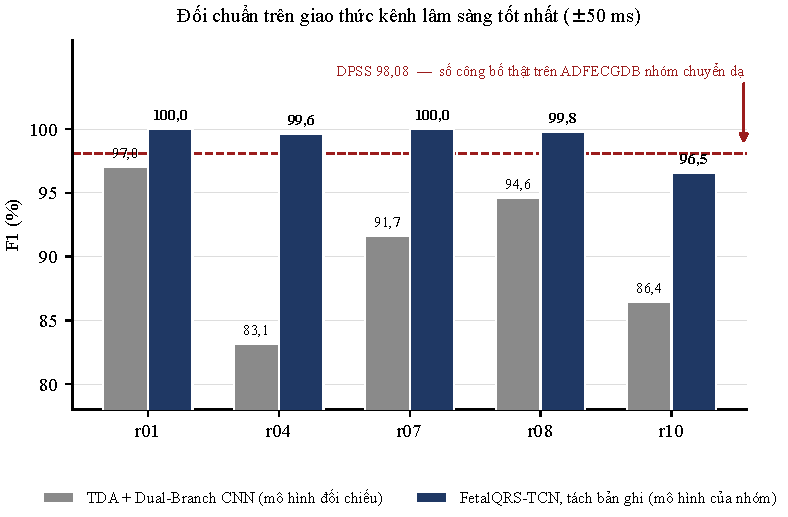
\includegraphics[width=0.94\textwidth]{figs/fig5_doi_chuan.pdf}
\caption{Đối chuẩn trên giao thức kênh lâm sàng tốt nhất, dung sai $\pm$50\,ms. Đường đứt đỏ là con số
\textbf{thật} mà bài DPSS công bố cho nhóm chuyển dạ.}
\label{fig:bench}
\end{figure}

Mô hình của nhóm đạt macro F1 \tot{99,18} theo bản đồ đạo trình quy định, so với 90,57 của mô hình đối
chiếu. Nhóm đã kiểm chứng lại bằng thuật toán khớp cặp tối ưu Hungarian độc lập: kết quả trùng khớp
tuyệt đối trên cả năm bản ghi, chênh lệch 0,00 điểm.

\subsection{Kiểm chứng các con số tham chiếu}

Nhóm đọc toàn văn 13 trang bài DPSS gốc để kiểm tra bảng tham chiếu trong gói đối chuẩn. Đây là việc
kiểm chứng học thuật thông thường giữa hai thành viên, mục đích là để báo cáo chung không chứa số liệu
sai.

\begin{table}[H]\centering\small
\caption{Kiểm chứng từng tuyên bố về ``kết quả đã công bố của DPSS''. Nguồn: Shokouhmand \& Tavassolian,
\textit{IEEE Trans.\ Biomed.\ Eng.} 70(1):283--295, 2023, DOI 10.1109/TBME.2022.3189617.}
\label{tab:kiemchung}
\begin{tabular}{@{}L{5.4cm} L{9.0cm}@{}}
\toprule
\textbf{Tuyên bố trong gói đối chuẩn} & \textbf{Đối chiếu với bài báo gốc} \\
\midrule
F1 theo từng bản ghi \texttt{r01}--\texttt{r10} & \xau{Không có nguồn.} Các định danh \texttt{r01},
\texttt{r04}, \texttt{r07}, \texttt{r08}, \texttt{r10} xuất hiện \textbf{0 lần} trong toàn văn. \\
Macro F1 91,03 & \xau{Không có nguồn.} Con số thật là \textbf{97,7\%} trên \textbf{22 tín hiệu}
(10 thai kỳ + 12 chuyển dạ), và \textbf{98,08\%} riêng nhóm chuyển dạ. \\
Sáu con số jitter (22,0--28,5\,ms) & \xau{Không có nguồn.} Bài không báo cáo jitter. Từ ``jittering''
trong bài là kỹ thuật tăng cường dữ liệu bằng nhiễu Gauss. \\
MAE fHR theo bpm & \xau{Không có nguồn.} Bài dùng chỉ số khác: ``FHR precision'' $=$ phần trăm cửa sổ có
fHR sai lệch trong $\pm$5\,bpm, đạt 88,61\%. \\
6.800.000 tham số, 55,0\,MB, $>$500\,MB RAM & \xau{Không có nguồn.} Bài không nêu bất kỳ con số nào
trong số này. \\
Độ trễ 35--50\,ms & \xau{Sai.} Con số thật là \textbf{0,52 giây} cho một cửa sổ 4 giây trên CPU Intel
3,6\,GHz. \\
``Bất khả thi Edge AI, cần máy chủ Cloud'' & \xau{Bài kết luận ngược lại.} DPSS đo được 1,2\,s trên
Raspberry Pi, 1,0\,s trên Apple S7, và bài kết luận DPSS ``phù hợp cho hệ thống theo dõi thai nhi thời
gian thực''. \\
Nhãn ``chuẩn AAMI EC57 $\pm$50\,ms'' & \xau{Nhãn sai.} Cụm ``AAMI'' và ``EC57'' xuất hiện \textbf{0 lần}
trong bài DPSS. Ngưỡng 50\,ms được trích từ Behar và cộng sự 2016. Chuẩn AAMI EC57 thật sự dùng cửa sổ
\textbf{150\,ms}. \\
\bottomrule
\end{tabular}
\end{table}

\begin{ghichu}[title={Điều đúng trong gói đối chuẩn}]
Nhóm ghi nhận rõ ba điểm:
\begin{enumerate}[leftmargin=1.5em,itemsep=2pt]
\item \textbf{Cột số liệu mô hình Persistence Image là số chạy máy thật.} Nhóm tái tạo được cả năm giá
trị MAE từ TP/FP/FN bằng chính công thức trong mã nguồn, khớp 5/5. Vấn đề nằm ở cột tham chiếu DPSS và
ở định nghĩa chỉ số, \textbf{không nằm ở phép đo mô hình của bạn ấy}.
\item Số nhịp nhãn chuẩn từng bản ghi (644/632/627/651/637, tổng 3.191) khớp tuyệt đối với tệp
\texttt{.qrs} gốc.
\item Bản đồ đạo trình được đề nghị là hợp lý về sinh lý, và trùng với quy tắc chọn kênh mù nhãn của
nhóm ở 2/5 bản ghi.
\end{enumerate}
\end{ghichu}

\subsection{Hai lỗi kỹ thuật trong mã đánh giá}

\paragraph{Hàm ghép cặp không phải song ánh.} Hàm \texttt{bipartite\_aami\_ec57\_matching} thực chất là
thuật toán tham lam duyệt theo thứ tự mảng. Phản ví dụ nhóm đã chạy: với nhãn chuẩn tại
$\{0, 60\}$ và dự đoán tại $\{50, 100\}$, dung sai 50, hàm trả TP $=1$ trong khi khớp cặp tối ưu cho
TP $=2$. Đảo thứ tự dự đoán thành $\{100, 50\}$ thì hàm lại trả TP $=2$. Kết quả phụ thuộc thứ tự mảng.

Tuy nhiên nhóm cũng ghi rõ: \textbf{trên dữ liệu thật, sai khác này bằng không}. Nhóm đã so tham lam với
Hungarian trên cả năm bản ghi và chênh lệch là 0,00 điểm. Đây là lỗi định danh thuật toán, không làm sai
kết quả đã đo.

\paragraph{Công thức MAE nhịp tim đo sai đại lượng.} Công thức trong mã rút gọn thành
\[
\text{MAE}_{\text{fHR}} = \frac{\bigl|\,N_{\text{dự đoán}} - N_{\text{chuẩn}}\,\bigr|}{5},
\]
tức chỉ đo \textbf{số lượng} nhịp, không đo \textbf{vị trí} nhịp. Nhóm dựng phản ví dụ và chạy thật:
một mô hình dự đoán \textbf{hoàn toàn ngẫu nhiên}, F1 chỉ 20,96\%, vẫn đạt MAE $= 0{,}00$\,bpm --- tức
``tốt hơn'' cả DPSS lẫn mô hình đối chiếu.

Nhóm đề nghị thay bằng định nghĩa tính theo khoảng RR trong từng đoạn 4 giây. Theo định nghĩa đúng đó,
mô hình của nhóm đạt MAE $0{,}34$\,bpm và ``FHR precision'' $98{,}39\%$ --- so với $89{,}22\%$ mà DPSS
thật sự công bố cho nhóm chuyển dạ.

\begin{table}[H]\centering\small
\caption{Đối chuẩn sau khi đã sửa các con số tham chiếu. Đây là bảng nhóm sẽ dùng trong bài báo.}
\label{tab:doichuan_sua}
\begin{tabular}{@{}L{4.6cm} C{2.5cm} C{2.4cm} C{2.2cm} C{2.4cm}@{}}
\toprule
\textbf{Hệ thống} & \textbf{F1} & \textbf{Bộ dữ liệu} & \textbf{Số kênh} & \textbf{Độ trễ} \\
\midrule
DPSS (TBME 2023) & 98,08 & ADFECGDB 22 ca & 1 & 520\,ms \\
Power-MF (Physiol Meas 2024) & $98{,}0 \pm 3{,}0$ & ADFECG B2, 12 ca & 4 & bài không nêu \\
Persistence Image + CNN & 90,57 & ADFECGDB 5 ca & 1 & 7,0\,ms \\
\textbf{\mh{} (nhóm)} & \tot{99,21} & ADFECGDB 5 ca & 1 & \tot{4,35\,ms} \\
\bottomrule
\end{tabular}
\end{table}

\begin{canhbao}[title={Cách đọc bảng \ref{tab:doichuan_sua} cho đúng}]
Bốn dòng này \textbf{không} đặt cạnh nhau được một cách nghiêm ngặt. DPSS huấn luyện trên dữ liệu tổng
hợp rồi áp thẳng sang ADFECGDB không tinh chỉnh, tức là con số tổng quát hoá xuyên miền --- khó hơn
hẳn. Power-MF dùng bốn kênh trên bộ Silesia ở 500\,Hz. Chỉ hai dòng cuối là cùng dữ liệu và cùng giao thức.

Nhóm đưa bảng này vào để cho thấy vị trí tương đối, và sẽ ghi rõ cảnh báo này trong bài báo thay vì
tuyên bố vượt trội.
\end{canhbao}

\clearpage

% ================================================================= C3: KẾT QUẢ PROTOTYPE
\section{Đóng góp C3 sau khi chạy prototype}
\label{sec:fsqi}

Bản đề cương trước đặt C3 là ``chỉ số chất lượng tín hiệu thai dựa trên đồng điều bền vững, có quyền
từ chối trả lời'' và thừa nhận nó chưa có một dòng dữ liệu nào. Nhóm đã xây prototype và chạy thí nghiệm
có kiểm soát. \textbf{Kết quả là phủ định cho phần đồng điều bền vững, và khẳng định cho phần từ chối
trả lời.} Mục này trình bày nguyên trạng.

\subsection{Thiết kế thí nghiệm}

Câu hỏi: \textit{đặc trưng topo tính trên từng đoạn 4 giây có dự báo được khi nào mô hình sẽ sai không,
và có hơn các chỉ số chất lượng cổ điển không?}

\begin{table}[H]\centering\small
\caption{Hai nhóm đặc trưng được so sánh. Mọi đặc trưng tính trên tín hiệu dư sau khử mẹ, 250\,Hz, đoạn
4 giây, chuẩn hoá robust. Mã tại \texttt{fsqi/fsqi.py}.}
\label{tab:fsqi_dactrung}
\begin{tabular}{@{}L{3.4cm} C{1.0cm} L{9.8cm}@{}}
\toprule
\textbf{Nhóm} & \textbf{Số} & \textbf{Nội dung} \\
\midrule
Topo --- Takens + ripser & 11 & Nhúng trễ chiều 3, $\tau = 20$\,ms, 300 điểm; tổng, cực đại, entropy và
số thanh persistence của $H_0$ và $H_1$ \\
Topo --- sublevel $H_0$ & 5 & Đồng điều $H_0$ của lọc dưới mức trên tín hiệu 1 chiều (đối chiếu với
\texttt{scipy} prominence: sai lệch 0,0 trên 2.011 đỉnh) \\
Cổ điển --- chỉ tín hiệu & 6 & SampEn, kurtosis, entropy phổ, tỉ lệ năng lượng 10--60\,Hz, đỉnh PSD dải
nhịp thai, trễ tự tương quan \\
Cổ điển --- đầu ra mô hình & 6 & CV khoảng RR, tỉ lệ RR hợp lý, bSQI, số đỉnh, xác suất trung bình tại
đỉnh, xác suất cực đại \\
\bottomrule
\end{tabular}
\end{table}

Giao thức chống rò rỉ: nhãn ``đoạn lỗi'' là F1 của mô hình trên đoạn đó dưới 80; bộ phân loại huấn luyện
\textbf{chỉ trên ADFECGDB} (1.500 đoạn, checkpoint fold đúng), kiểm thử \textbf{xuyên miền trên CinC 2013}
(600 đoạn, checkpoint production, zero-shot). Không chọn siêu tham số bằng nhãn kiểm thử. Bootstrap 1.000
lần theo đoạn và theo cụm bản ghi. Hai lần chạy độc lập cho kết quả trùng khớp 1.327/1.327 trường.

\subsection{Kết quả}

\begin{table}[H]\centering\small
\caption{Dự báo đoạn lỗi trên CinC 2013 (ngoài miền), bộ phân loại huấn luyện trên ADFECGDB. Cột cuối:
macro F1 của các đoạn được giữ lại sau khi từ chối 20\% đoạn kém tin cậy nhất.}
\label{tab:fsqi_kq}
\begin{tabular}{@{}L{4.6cm} C{1.9cm} C{1.9cm} C{2.3cm} C{2.3cm}@{}}
\toprule
\textbf{Nhóm đặc trưng} & \textbf{AUROC} & \textbf{AUPRC} & \textbf{F1, phủ 80\%} & \textbf{F1, phủ 50\%} \\
\midrule
Từ chối ngẫu nhiên (đường cơ sở) & 0,500 & $\approx$0,52 & 62,03 & 62,14 \\
\textbf{Topo} (16 đặc trưng) & \xau{0,566} & 0,564 & 63,40 & 64,44 \\
Cổ điển, chỉ tín hiệu (6) & 0,666 & 0,686 & --- & --- \\
\textbf{Cổ điển} (12) & \tot{0,929} & 0,927 & \tot{69,40} & \tot{84,51} \\
Kết hợp topo + cổ điển (28) & 0,905 & 0,899 & 69,41 & 82,44 \\
Oracle (biết F1 thật) & --- & --- & 74,55 & 97,81 \\
\bottomrule
\end{tabular}
\end{table}

\begin{figure}[H]\centering
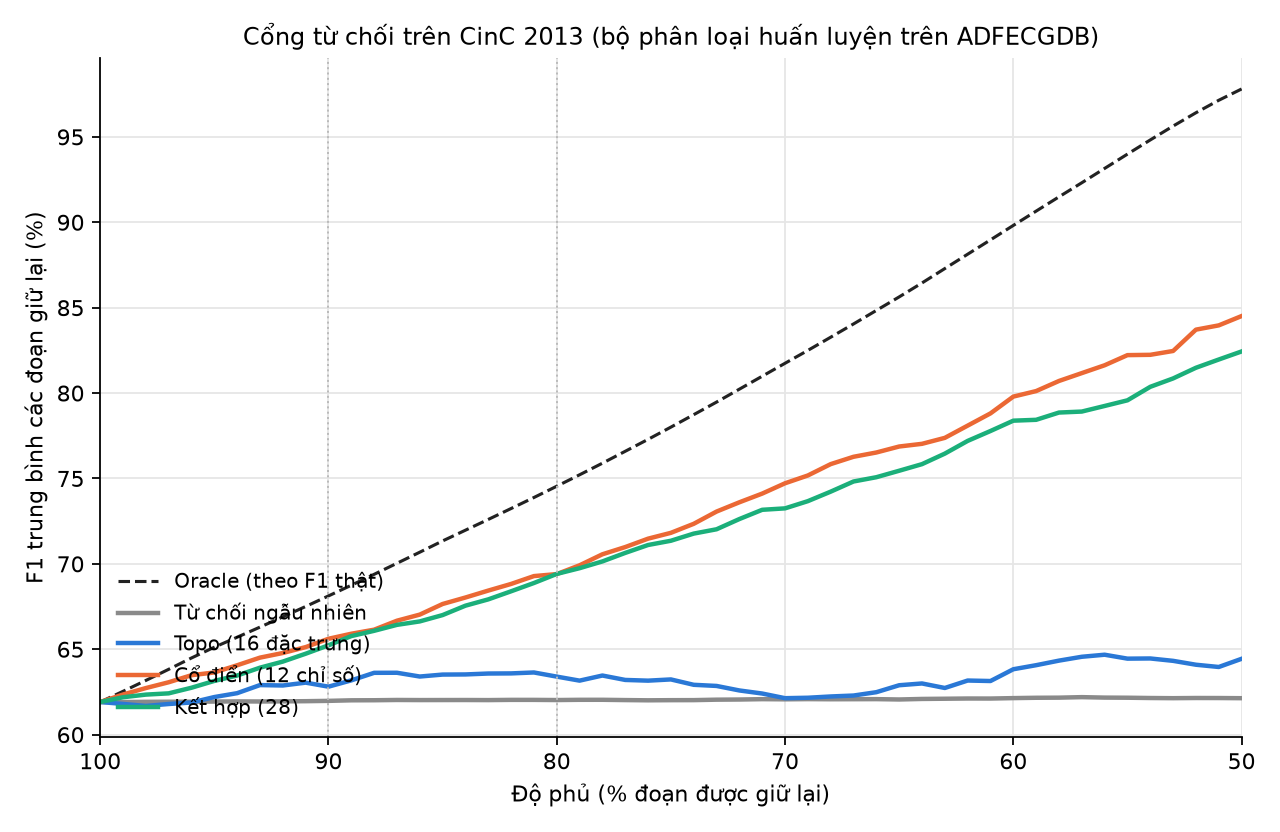
\includegraphics[width=0.92\textwidth]{figs/fig9_risk_coverage.png}
\caption{Đường cong rủi ro--độ phủ trên CinC 2013. Đường topo (xanh dương) gần như nằm sát đường từ chối
ngẫu nhiên (xám) trên toàn bộ dải độ phủ. Đường cổ điển (cam) tách rõ và tiến về oracle (đứt).}
\label{fig:riskcov}
\end{figure}

\begin{figure}[H]\centering
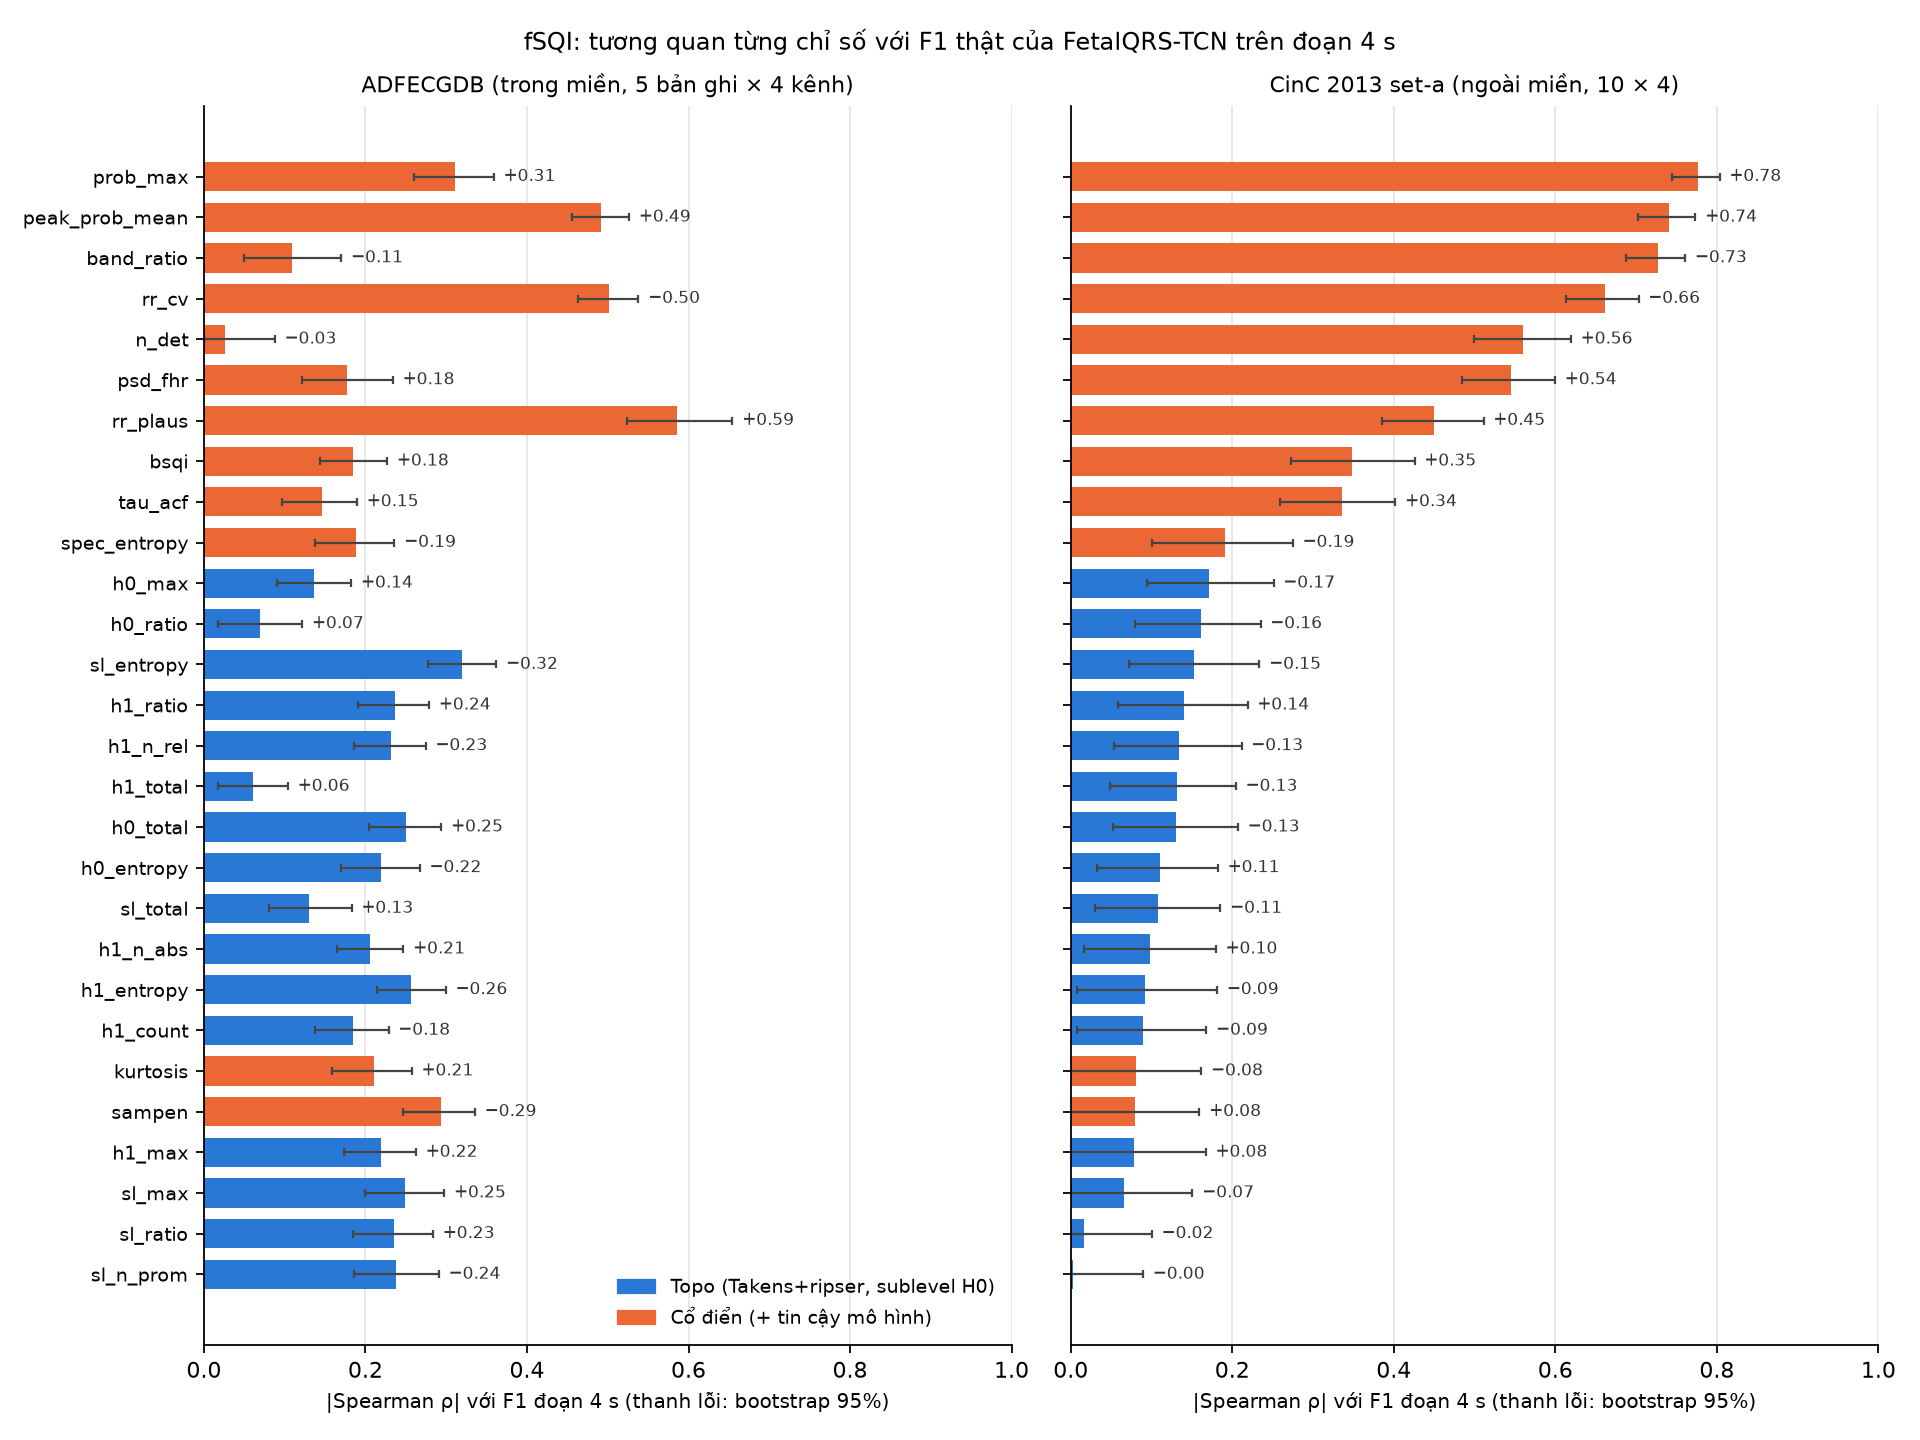
\includegraphics[width=\textwidth]{figs/fig10_sqi_correlation.png}
\caption{Tương quan Spearman của từng chỉ số với F1 đoạn, kèm khoảng tin cậy bootstrap 95\%. Trái: trong
miền. Phải: ngoài miền. Các chỉ số cổ điển (cam) \textbf{mạnh lên} khi ra ngoài miền; các chỉ số topo
(xanh) \textbf{yếu đi} và nhiều chỉ số đổi dấu.}
\label{fig:sqicorr}
\end{figure}

\subsection{Đọc kết quả}

\begin{enumerate}[leftmargin=1.6em,itemsep=5pt]
\item \textbf{Topo không dự báo được lỗi ở mức hữu dụng.} AUROC 0,566 gần ngẫu nhiên. Cổng từ chối dựa
trên topo chỉ hơn từ chối ngẫu nhiên 1,4 điểm ở độ phủ 80\%. Trong miền có tín hiệu yếu ($\rho = -0{,}32$
cho entropy sublevel), nhưng tín hiệu đó \textbf{không chuyển miền được}: bốn đặc trưng topo đổi dấu
tương quan giữa ADFECGDB và CinC.

\item \textbf{Topo không bổ sung gì cho cổ điển.} Gộp 28 đặc trưng cho AUROC 0,905, \textit{thấp hơn} 12
đặc trưng cổ điển đơn thuần (0,929). Thêm topo vào là thêm nhiễu.

\item \textbf{Ngay cả chỉ số cổ điển thuần tín hiệu cũng hơn topo} (0,666 so với 0,566), dù không dùng
đầu ra mô hình.

\item \textbf{Cổng từ chối có tác dụng thật, nhưng bằng chỉ số khác.} Chỉ số dự báo lỗi mạnh nhất là
\textbf{độ tự tin của chính mô hình} (\texttt{prob\_max}, AUROC đơn lẻ 0,970) và \textbf{độ đều của nhịp}
(\texttt{rr\_cv}, 0,915). Chỉ số thuần tín hiệu tốt nhất là \textbf{tỉ lệ năng lượng 10--60\,Hz}
(0,904) --- lần thứ ba dải tần này xuất hiện như biến quan trọng nhất của đề tài.

\item \textbf{Chi phí tính topo không phải rào cản.} Trung bình 65\,ms mỗi đoạn, p95 80\,ms. Vấn đề không
phải tốc độ mà là thông tin.
\end{enumerate}

\begin{canhbao}[title={Con số 0,929 trả lời sai câu hỏi --- đính chính bắt buộc của bản 3.3}]
600 đoạn 4 giây trong bảng trên đến từ \textbf{10 bản ghi}, và đoạn trong cùng một bản ghi tương quan
mạnh. Tính lại với cluster bootstrap \textbf{theo bản ghi} ($n = 10$ cụm): AUROC $= 0{,}929$
$[0{,}830;\ 0{,}982]$.

Quan trọng hơn: \textbf{5/10 bản ghi CinC không có đoạn xấu nào}, nên chúng không đóng góp gì vào AUROC
gộp. Con số 0,929 vì vậy phần lớn trả lời câu hỏi \textit{``bản ghi này có phải bản ghi xấu không''}.
Câu hỏi mà cổng từ chối được bán như là thứ trả lời --- \textit{``đoạn 4 giây này trong bản ghi của bệnh
nhân này có đáng tin không''} --- có đáp số là \textbf{AUROC TRONG bản ghi $= 0{,}721$}
$[0{,}517;\ 0{,}898]$, trung bình trên 5 bản ghi có cả đoạn tốt lẫn đoạn xấu (a01 $= 0{,}914$;
a06 $= 0{,}390$; a07 $= 0{,}889$; a09 $= 0{,}886$; a10 $= 0{,}526$).

Kết luận phủ định về topo \textbf{không đổi} (0,566 so với 0,929 hay so với 0,721 đều là thua). Nhưng
tuyên bố khẳng định về cổng từ chối phải hạ xuống: nó \textbf{chưa} dùng được ở mức đoạn tại giường bệnh.
Chi tiết ở \S\ref{sec:thongke}.
\end{canhbao}

\begin{canhbao}[title={Điều này làm gì với đóng góp C3}]
Nhóm \textbf{rút lại} phần ``dựa trên đồng điều bền vững'' trong phát biểu C3. Đây là lần thứ ba trong đề
tài mà phân tích dữ liệu topo được kiểm chứng có kiểm soát và không mang lại lợi ích: (1) Persistence
Image làm đặc trưng dò đỉnh đứng chót 16 kiến trúc; (2) sublevel $H_0$ trùng 100\% với độ nhô đỉnh cổ
điển; (3) đặc trưng topo làm chỉ số chất lượng đạt AUROC 0,566 so với 0,929 của chỉ số cổ điển.

\textbf{C3 được phát biểu lại thành:} \textit{cổng từ chối trả lời cho bộ dò fQRS đơn kênh, xây trên độ
tự tin của mô hình và tính hợp lý của nhịp, kèm một kết quả phủ định có kiểm soát về đồng điều bền vững
trong vai trò chỉ số chất lượng tín hiệu thai.}

Giả thuyết H0 trong bản đề cương trước đã dự phòng đúng tình huống này: kết quả phủ định có kiểm định,
với đối chứng ngẫu nhiên và oracle, huấn luyện--kiểm thử xuyên miền, không chọn siêu tham số bằng nhãn
kiểm thử, là một đóng góp công bố được.
\end{canhbao}

\subsection{Vì sao topo thất bại ở đây}

Nhóm đưa ra ba lý do, đánh dấu rõ mức chắc chắn:

\begin{description}[leftmargin=2.0em,style=nextline,itemsep=4pt]
\item[Đã chứng minh --- sublevel $H_0$ không phải đặc trưng mới.] Định lý Elder cho biết persistence của
mỗi thanh $H_0$ đúng bằng độ nhô của một đỉnh. Nhóm đã kiểm chứng sai lệch 0,0 trên 2.011 đỉnh. Nên
nhóm 5 đặc trưng này chỉ là cách viết lại thống kê độ nhô, và độ nhô đã nằm trong bộ chỉ số cổ điển.

\item[Đã đo --- đặc trưng $H_1$ của nhúng trễ không ổn định giữa bộ dữ liệu.] Hình \ref{fig:sqicorr} cho
thấy dấu tương quan đổi chiều. Cấu trúc vòng trong không gian nhúng phụ dấu vào biên độ tương đối của
sóng mẹ còn sót và nhiễu cơ, hai thứ khác hẳn giữa hai bộ dữ liệu.

\item[Suy luận --- lỗi mô hình là lỗi \textit{nhịp}, không phải lỗi \textit{hình dạng}.] Ảnh chụp demo
trên a02 (hình \ref{fig:demo_a02}) cho thấy cơ chế thất bại chính: mô hình bám nhầm vào nhịp mẹ. Đó là
lỗi ở thang thời gian hàng giây, trong khi đặc trưng topo trên đoạn 4 giây mô tả hình dạng ở thang mili
giây. Hai thang không gặp nhau. Đây là lý do độ đều nhịp và tỉ lệ trùng đỉnh mẹ dự báo lỗi tốt hơn nhiều.
\end{description}

\subsection{Giới hạn của thí nghiệm này}

CinC 2013 set-a chỉ có 10 bản ghi $\times$ 1 phút, lỗi tập trung theo bản ghi nên khoảng tin cậy theo cụm
rộng hơn nhiều so với theo đoạn. Chỉ một cấu hình topo được thử (chiều 3, $\tau = 20$\,ms, 300 điểm) và
nhóm \textbf{cố ý không quét} tham số để tránh chọn theo nhãn kiểm thử --- nên chưa loại trừ hoàn toàn
khả năng một cấu hình khác tốt hơn. Bộ phân loại kết hợp (0,905) thấp hơn cả \texttt{prob\_max} đơn lẻ
(0,970), tức một ngưỡng đơn có thể là cổng tốt hơn bộ học, và điều này chưa được đo riêng.

\clearpage
% ================================================================= DEMO VÀ ĐÈN TIN CẬY
\section{Bản demo và đèn tin cậy}
\label{sec:demo}

Nhóm đã xây bản demo chạy được, tách thành hai tầng: \texttt{demo/core.py} chứa toàn bộ logic, không phụ
thuộc thư viện giao diện và có bộ kiểm thử riêng; \texttt{demo/app.py} là giao diện web một trang bằng
Gradio, chạy trên máy cá nhân bằng lệnh \texttt{python demo/app.py}.

\subsection{Bố cục}

Màn hình gồm bốn khối, xếp theo thứ tự người xem cần biết:

\begin{enumerate}[leftmargin=1.6em,itemsep=3pt]
\item \textbf{Đầu vào}: tải tệp EDF/WFDB/CSV hoặc chọn bản ghi mẫu; chọn kênh tự động (quy tắc PSD mù
nhãn) hoặc thủ công. Nếu chọn bản ghi ADFECGDB thì hệ thống \textit{tự động} dùng checkpoint chưa từng
thấy bản ghi đó, để kết quả hiển thị là kết quả trung thực.
\item \textbf{Tín hiệu qua từng bước}, năm tab: thô, đã lọc kèm vạch nhịp mẹ, sau khử mẹ kèm vạch nhịp
thai thật nếu có nhãn, xác suất từng mẫu kèm ngưỡng, và kết quả. Người xem kéo thả phóng to được.
\item \textbf{Nhịp tim thai theo thời gian}, tô vùng bình thường 110--160 nhịp/phút.
\item \textbf{Bốn thẻ số}: nhịp tim trung bình, số nhịp, \textbf{đèn tin cậy}, thời gian xử lý. Nếu có
nhãn thì hiện thêm Se/PPV/F1/jitter.
\end{enumerate}

Chân trang cố định: \textit{``Bản mẫu nghiên cứu. Không phải thiết bị y tế. Không dùng cho chẩn đoán.''}

\begin{figure}[H]\centering
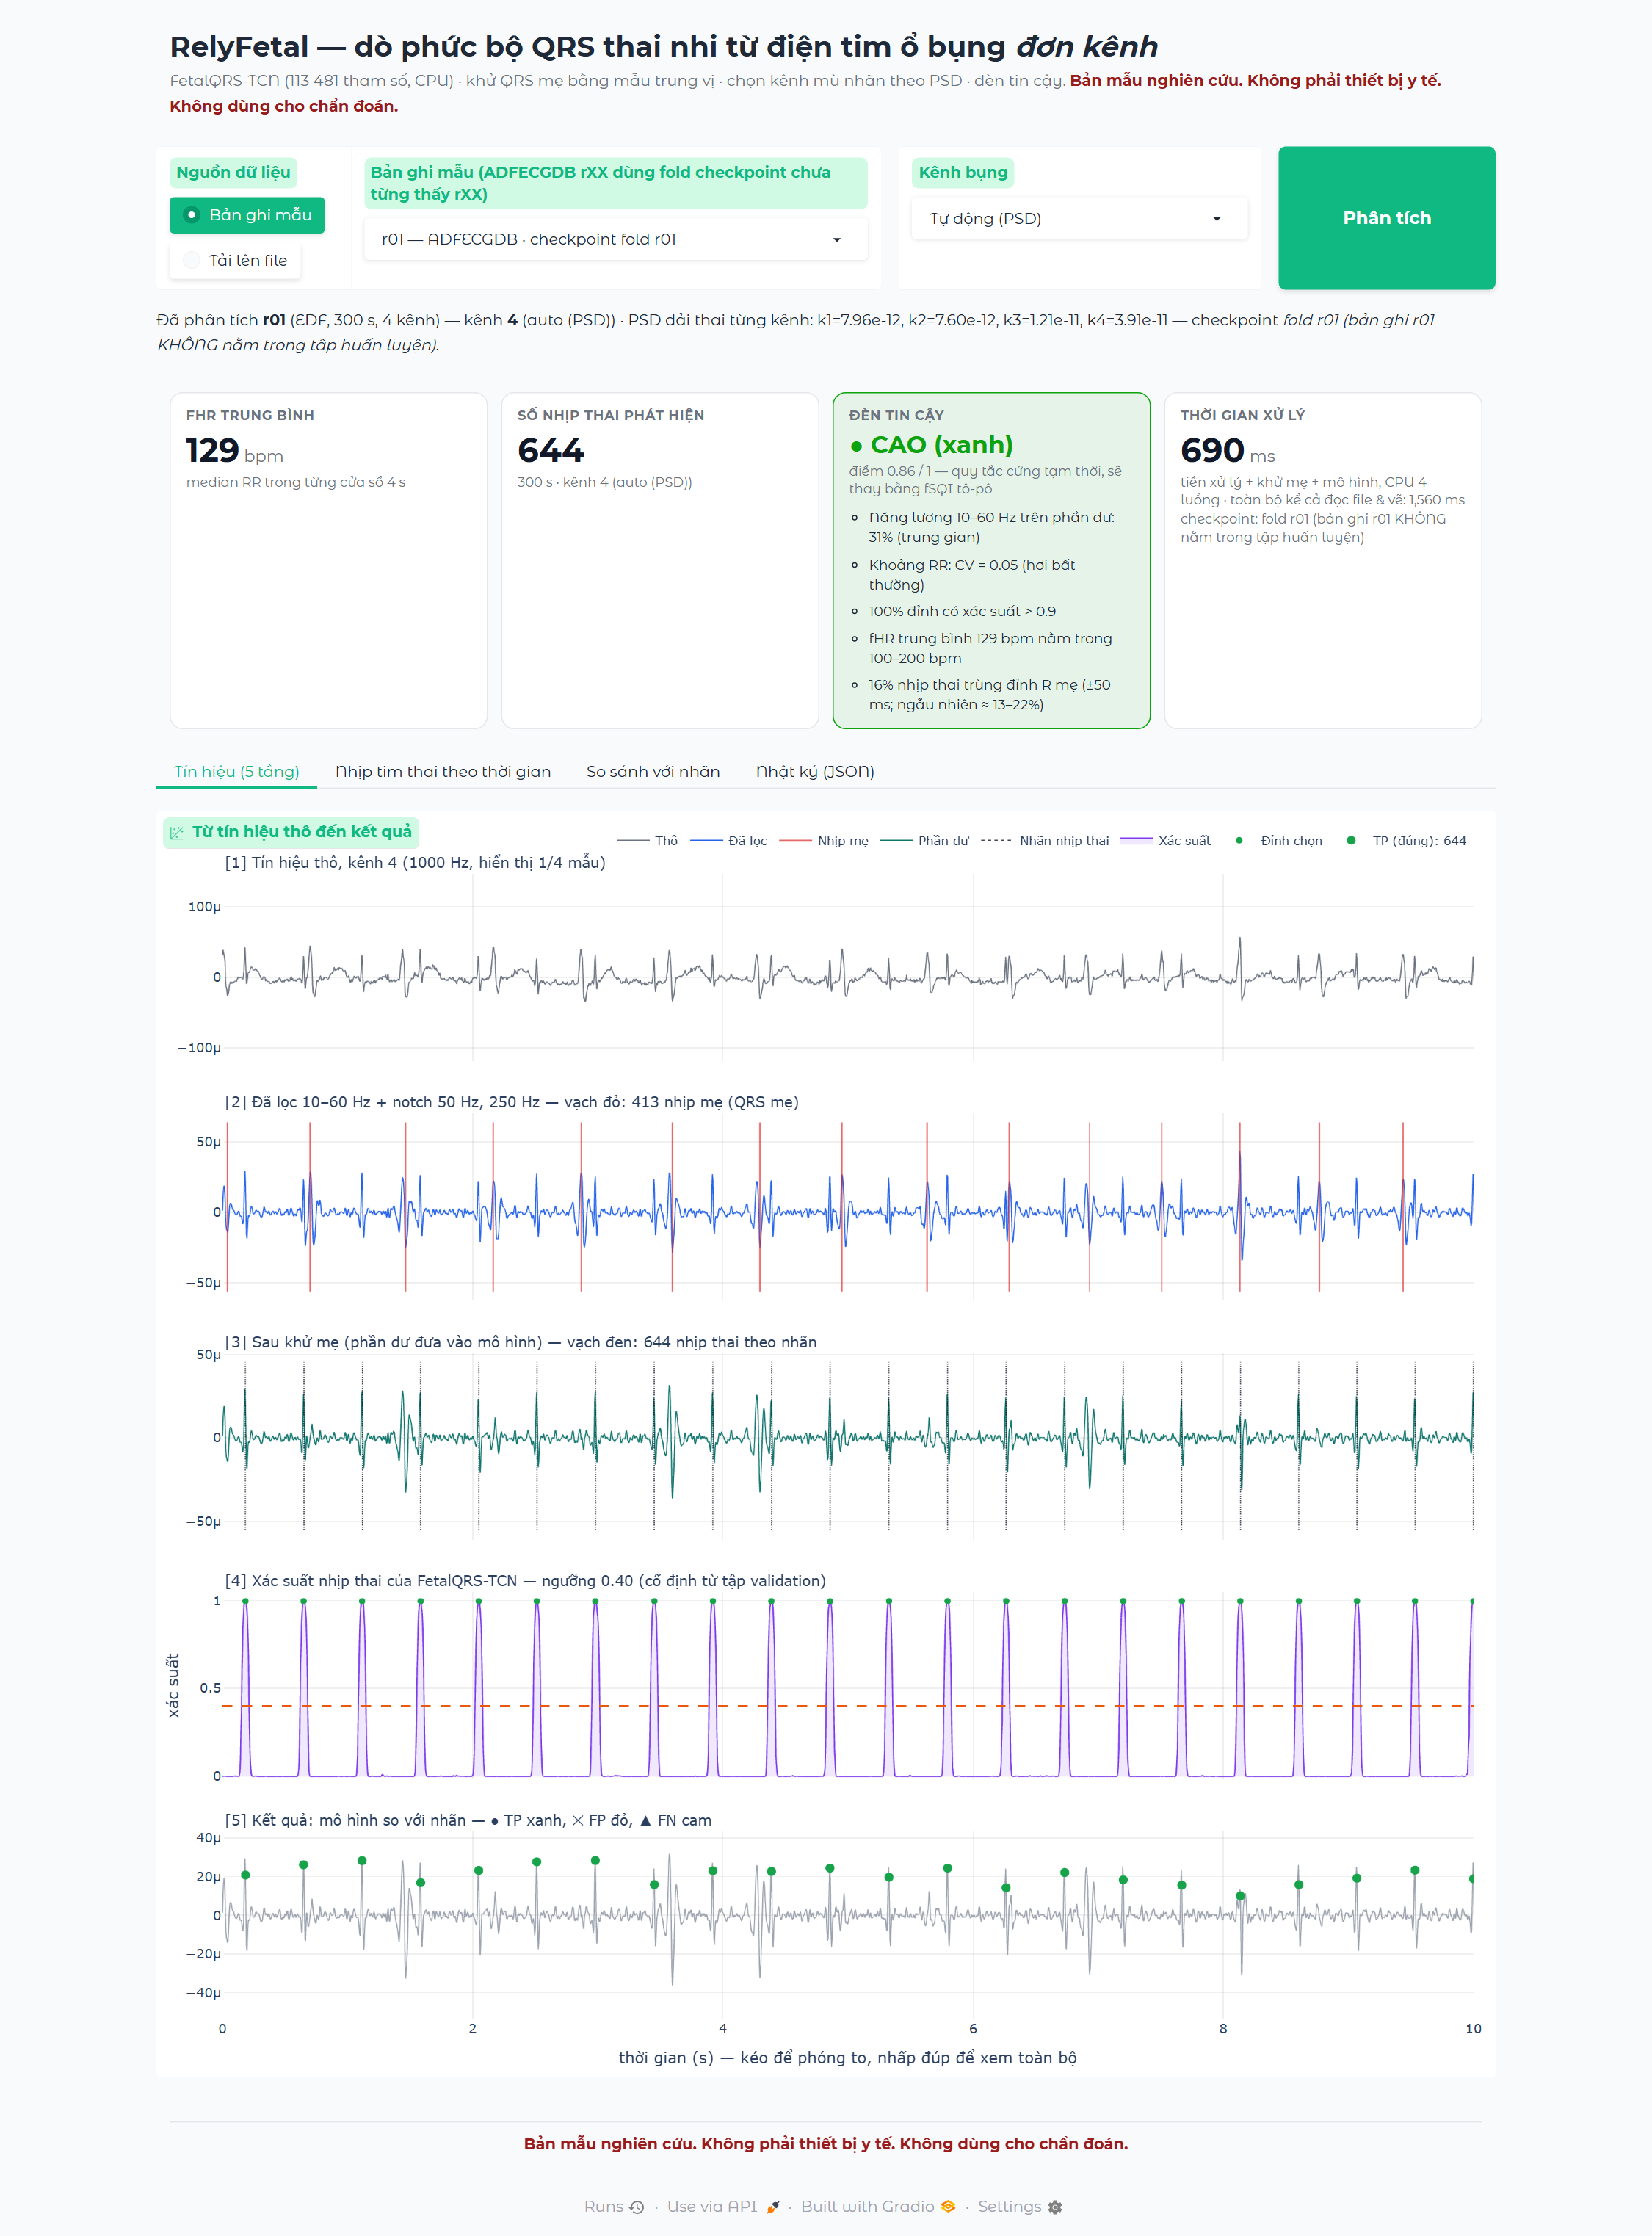
\includegraphics[width=0.92\textwidth]{figs/fig11_demo_r01.png}
\caption{Ảnh chụp giao diện thật trên r01, kênh chọn tự động, checkpoint chưa thấy r01. Năm tầng tín
hiệu, 644 nhịp, đèn xanh, 690\,ms xử lý cho 5 phút tín hiệu.}
\label{fig:demo_r01}
\end{figure}

\begin{figure}[H]\centering
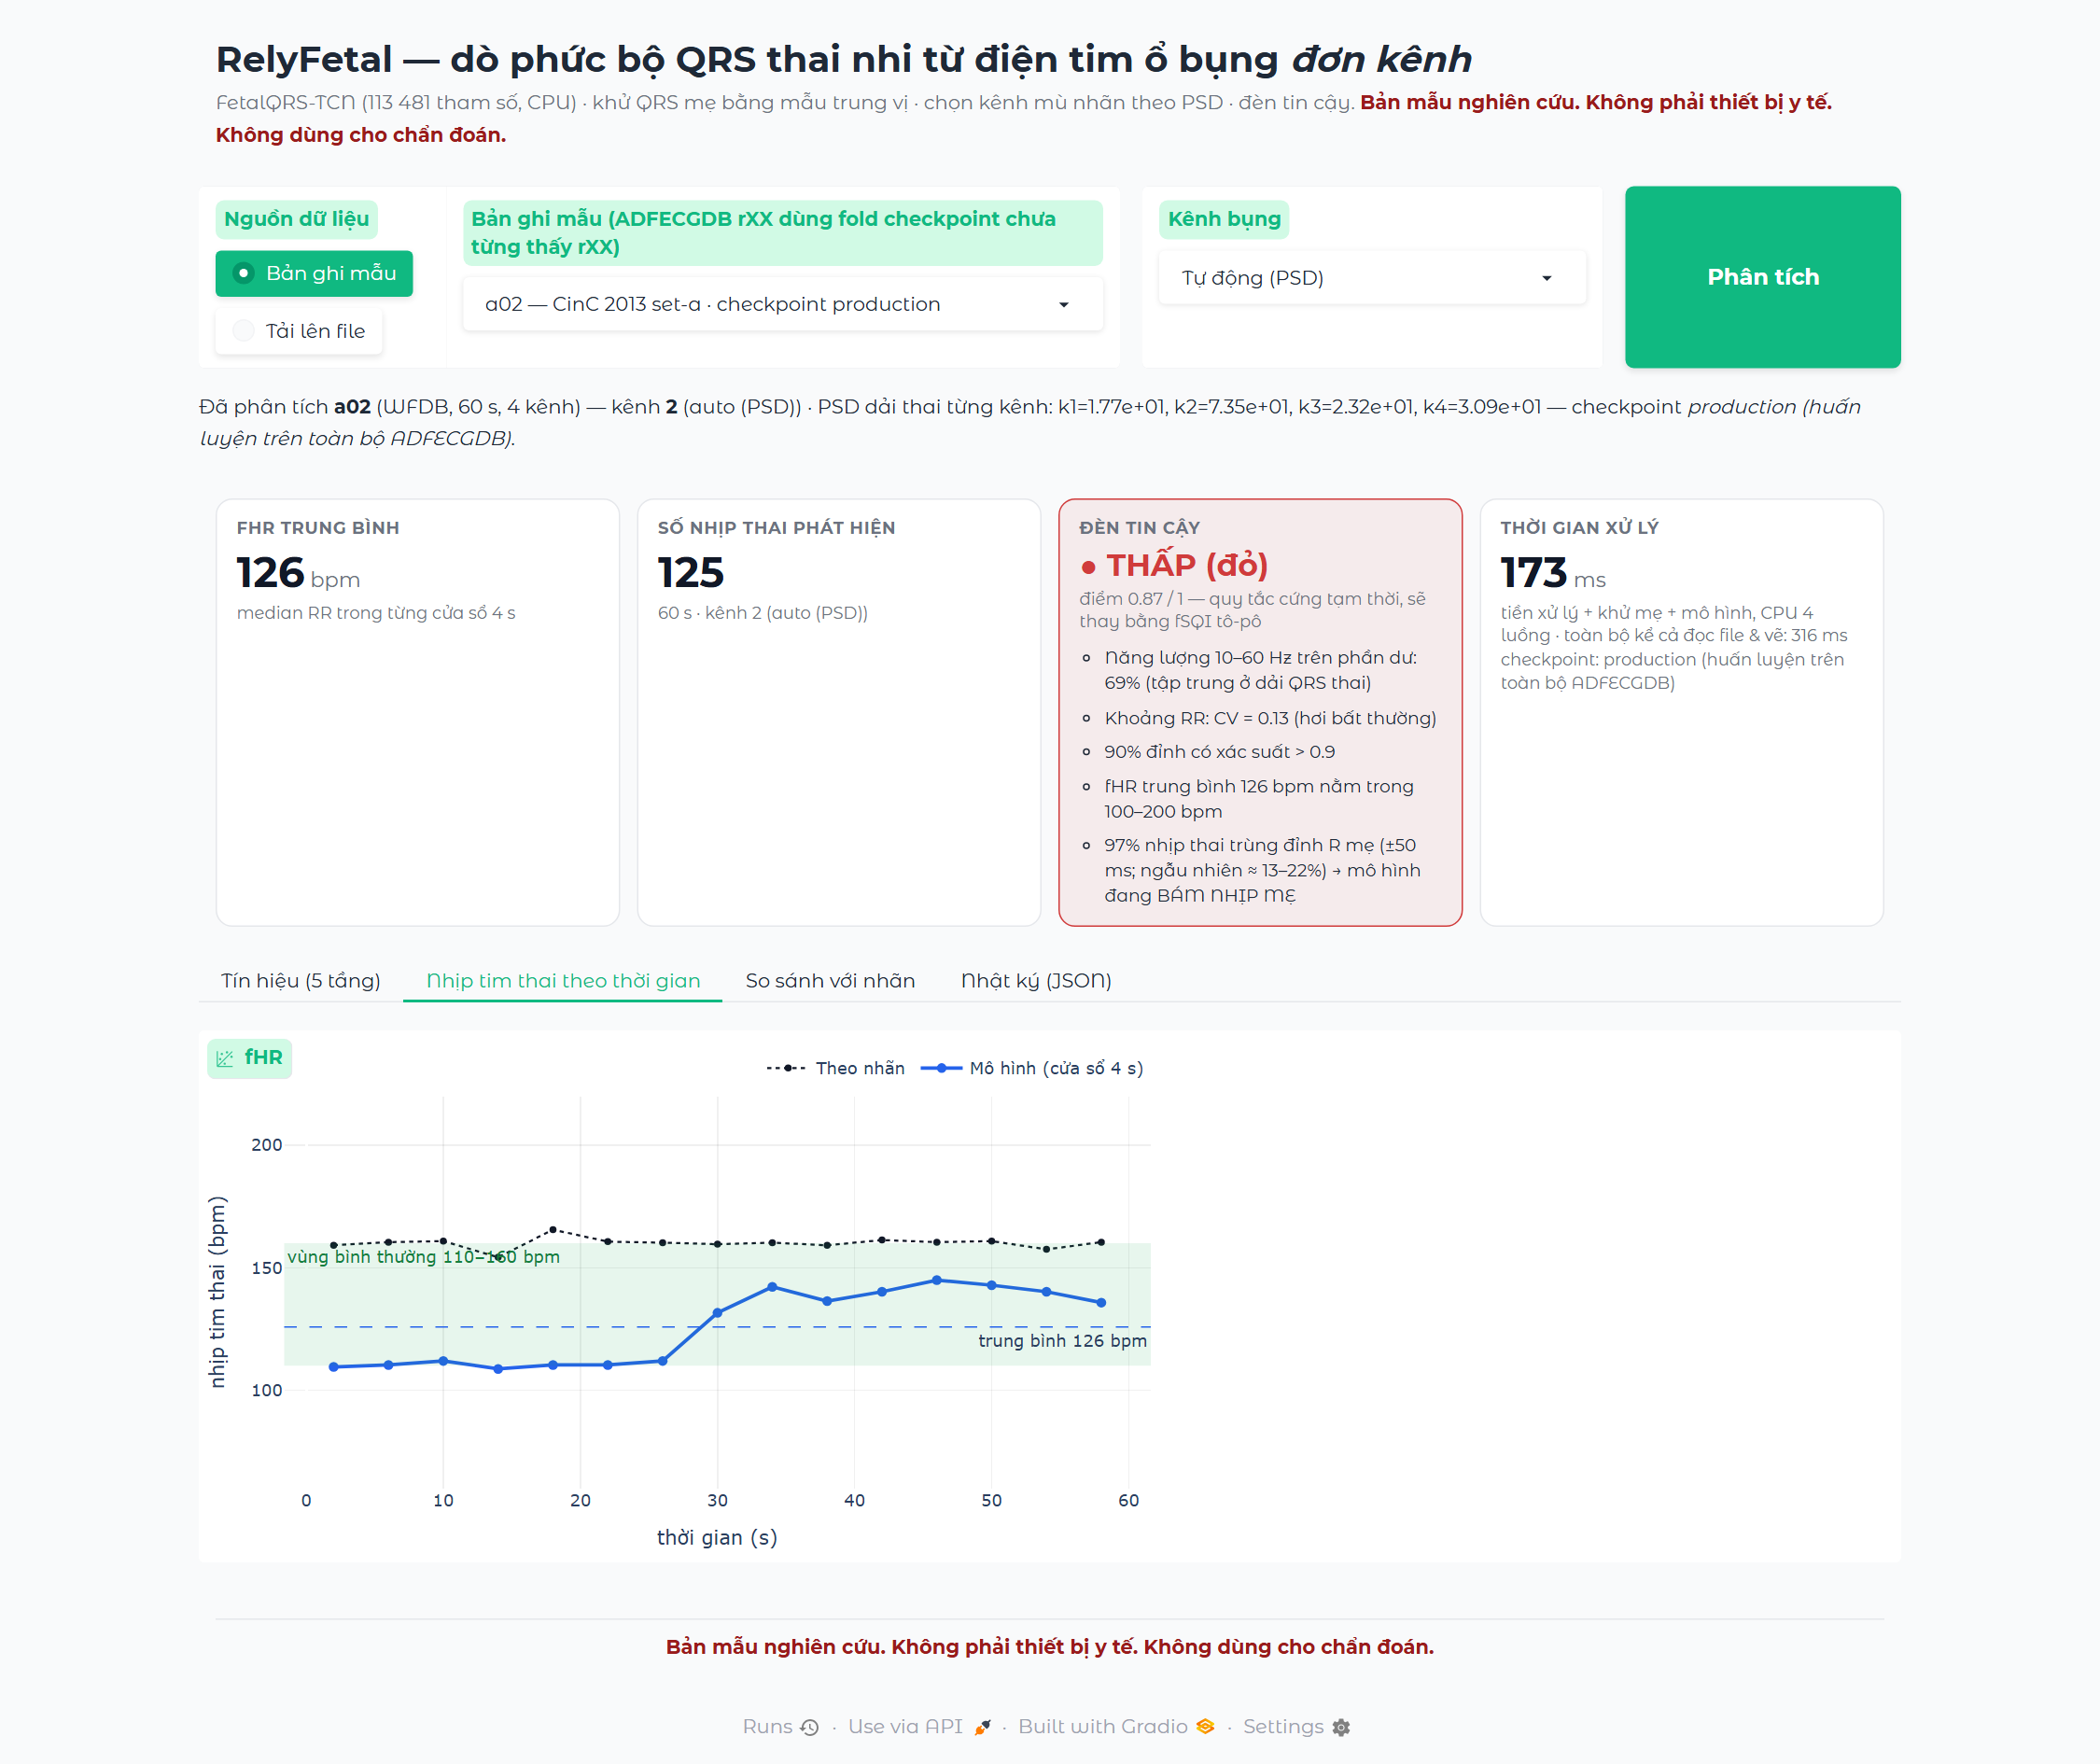
\includegraphics[width=0.92\textwidth]{figs/fig12_demo_a02.png}
\caption{Ảnh chụp trên a02, bản ghi tệ nhất của CinC 2013, zero-shot. Đèn \textbf{đỏ} vì 97\% nhịp
``thai'' trùng đỉnh R mẹ. Đồ thị nhịp tim cho thấy đúng cơ chế thất bại: đường mô hình bám ở nhịp mẹ
($\approx$126) trong khi nhãn ở $\approx$160 nhịp/phút. Hệ thống tự phát hiện và từ chối, thay vì báo
sai.}
\label{fig:demo_a02}
\end{figure}

\subsection{Đèn tin cậy}

Đây là thành phần biến demo từ ``một bộ dò QRS nữa'' thành thứ khác biệt. Phiên bản hiện tại dùng
\textbf{luật cứng} kết hợp bốn dấu hiệu, mỗi dấu hiệu chỉ dùng chính tín hiệu và đầu ra mô hình, không
dùng nhãn:

\begin{table}[H]\centering\small
\caption{Bốn dấu hiệu của đèn tin cậy phiên bản luật cứng. Trọng số cộng lại thành điểm 0--1; xanh nếu
$\geq 0{,}75$, vàng nếu $\geq 0{,}45$, đỏ nếu thấp hơn. Có một luật ghi đè: nếu hơn 60\% nhịp ``thai''
trùng đỉnh R mẹ thì đèn đỏ bất kể điểm, vì đó là dấu hiệu bộ dò đang bám nhầm vào tim mẹ.}
\label{tab:dentincay}
\begin{tabular}{@{}L{4.6cm} L{6.6cm} C{1.6cm}@{}}
\toprule
\textbf{Dấu hiệu} & \textbf{Ý nghĩa} & \textbf{Trọng số} \\
\midrule
Tỉ lệ năng lượng 10--60\,Hz trên phần dư & Phần dư còn chứa QRS thai hay chỉ còn nhiễu & 0,2 \\
Hệ số biến thiên khoảng RR & Nhịp đều là dấu hiệu bắt đúng; nhịp loạn là dấu hiệu bắt nhiễu & 0,3 \\
Tỉ lệ đỉnh có xác suất $> 0{,}9$ & Mô hình có tự tin vào các đỉnh nó chọn không & 0,3 \\
Nhịp tim nằm trong 100--200 nhịp/phút & Kiểm tra sinh lý & 0,2 \\
\bottomrule
\end{tabular}
\end{table}

Luật này được cố định trước khi chạy, rồi chấm trên 15 bản ghi có nhãn.

\begin{table}[H]\centering\small
\caption{Đèn tin cậy chấm trên 15 bản ghi có nhãn, kênh chọn tự động. ADFECGDB dùng checkpoint chưa
thấy bản ghi; CinC 2013 dùng checkpoint production, zero-shot.}
\label{tab:den15}
\begin{tabular}{@{}L{1.4cm} L{2.0cm} C{1.0cm} C{1.6cm} C{2.0cm} C{1.4cm} C{2.0cm}@{}}
\toprule
\textbf{Bản ghi} & \textbf{Bộ} & \textbf{Kênh} & \textbf{F1 thật} & \textbf{Đèn} & \textbf{Điểm} &
\textbf{Độ trễ} \\
\midrule
r01 & ADFECGDB & 4 & 100,00 & \tot{xanh} & 0,86 & 758\,ms \\
r04 & ADFECGDB & 2 & 99,76 & vàng & 0,74 & 778\,ms \\
r07 & ADFECGDB & 2 & 100,00 & \tot{xanh} & 0,80 & 661\,ms \\
r08 & ADFECGDB & 4 & 99,77 & \tot{xanh} & 0,90 & 720\,ms \\
r10 & ADFECGDB & 1 & 96,54 & \tot{xanh} & 0,92 & 732\,ms \\
\midrule
a03 & CinC 2013 & 1 & 100,00 & \tot{xanh} & 0,99 & 124\,ms \\
a04 & CinC 2013 & 4 & 100,00 & \tot{xanh} & 0,94 & 131\,ms \\
a05 & CinC 2013 & 4 & 100,00 & \tot{xanh} & 0,94 & 137\,ms \\
a08 & CinC 2013 & 4 & 100,00 & \tot{xanh} & 1,00 & 144\,ms \\
a01 & CinC 2013 & 2 & 59,18 & vàng & 0,57 & 118\,ms \\
a06 & CinC 2013 & 1 & 42,75 & vàng & 0,48 & 119\,ms \\
a07 & CinC 2013 & 2 & 29,82 & vàng & 0,48 & 125\,ms \\
a10 & CinC 2013 & 2 & 21,05 & vàng & 0,63 & 127\,ms \\
a02 & CinC 2013 & 2 & 21,75 & \xau{đỏ} & 0,87$^{*}$ & 132\,ms \\
a09 & CinC 2013 & 2 & 16,96 & \xau{đỏ} & 0,27 & 127\,ms \\
\bottomrule
\multicolumn{7}{@{}l}{\scriptsize $^{*}$ điểm cao nhưng bị luật ghi đè: 89\% nhịp ``thai'' trùng đỉnh R
mẹ --- bộ dò bám nhầm vào tim mẹ.}
\end{tabular}
\end{table}

\begin{table}[H]\centering\small
\caption{Tổng hợp theo màu đèn.}
\label{tab:den_tonghop}
\begin{tabular}{@{}C{2.0cm} C{2.2cm} C{2.6cm} C{2.6cm} C{2.6cm}@{}}
\toprule
\textbf{Đèn} & \textbf{Số bản ghi} & \textbf{F1 trung bình} & \textbf{F1 thấp nhất} & \textbf{F1 cao nhất} \\
\midrule
\tot{Xanh} & 8 & \textbf{99,54} & 96,54 & 100,00 \\
Vàng & 5 & 50,51 & 21,05 & 99,76 \\
\xau{Đỏ} & 2 & 19,36 & 16,96 & 21,75 \\
\bottomrule
\end{tabular}
\end{table}

\begin{ghichu}[title={Điều quan trọng nhất trong bảng \ref{tab:den_tonghop}}]
\textbf{Không có bản ghi nào bị đèn xanh mà F1 dưới 96.} Tức là luật cứng đơn giản này, dù chưa dùng
đặc trưng topo, đã đạt tính chất cần thiết nhất của một cổng an toàn: \textit{khi nó nói ``tin được'' thì
tin được}. Sai số duy nhất là theo chiều thận trọng --- r04 bị đèn vàng dù F1 là 99,76.

Trên CinC 2013, nếu chỉ trả lời khi đèn xanh thì macro F1 của phần được trả lời là \textbf{100,00}
trên 4/10 bản ghi, và hệ thống \textit{từ chối} 6 bản ghi còn lại thay vì báo sai. Đây là minh hoạ cụ thể
cho đóng góp C3 trước khi thay luật cứng bằng chỉ số topo học được.
\end{ghichu}

\subsection{Kịch bản trình bày ba phút}

\begin{table}[H]\centering\small
\caption{Kịch bản demo. Phút cuối là phần quan trọng nhất.}
\label{tab:kichban}
\begin{tabular}{@{}C{1.6cm} L{5.2cm} L{7.4cm}@{}}
\toprule
\textbf{Thời điểm} & \textbf{Thao tác} & \textbf{Điều cần nói} \\
\midrule
0:00--0:30 & Nạp r01, bấm Phân tích & Năm phút tín hiệu, xử lý xong dưới một giây \\
0:30--1:30 & Lướt năm tab tín hiệu & Đây là chỗ nhịp thai bị chôn; đây là sau khi trừ mẹ \\
1:30--2:00 & Bật so sánh với nhãn & 644 nhịp, không sót, không thừa, F1 100 \\
2:00--3:00 & \textbf{Nạp a02, bản ghi tệ nhất} & Đèn chuyển đỏ. Hệ thống tự biết nó bám nhầm tim mẹ và
từ chối trả lời, thay vì báo một con số sai \\
\bottomrule
\end{tabular}
\end{table}

Demo chỉ chạy trên ca đẹp thì ai cũng làm được. Demo dám chạy trên ca xấu và \textit{tự thừa nhận} mới
là điểm khác biệt.

\clearpage
% ================================================================= CHỈ SỐ LÂM SÀNG
\section{Chỉ số lâm sàng: hệ thống này dùng được đến đâu ở giường bệnh}
\label{sec:clinical}

F1 dò nhịp là chỉ số của người làm xử lý tín hiệu. Bác sĩ không quyết định gì dựa trên F1. Mục này đo
bốn đại lượng mà một máy theo dõi tim thai thật sự phải trả lời, trên \textbf{32 bản ghi, 269,6 phút tín
hiệu thật}: biến thiên ngắn hạn kiểu Dawes--Redman (STV), sai số nhịp tim thai theo Bland--Altman, độ phủ
theo \textbf{thời lượng}, và tần suất khoá nhầm nhịp mẹ. Mã tại \texttt{analysis/clinical.py}, số liệu
từng bản ghi tại \texttt{analysis/clinical\_results.json}.

\begin{canhbao}[title={Kết luận đặt ngay đầu mục, trước mọi con số}]
\textbf{Bộ dò này KHÔNG dùng được làm máy đo STV độc lập.} Trên tập con duy nhất đủ dài cho một trị số
Dawes--Redman hợp lệ (10 bản ghi Silesia B1, 20 phút mỗi bản), giới hạn đồng thuận 95\% là
$[-4{,}45;\ +8{,}14]$\,ms quanh một ranh giới quyết định mà hai mốc lâm sàng 2,6 và 3,0\,ms chỉ cách nhau
\textbf{0,4\,ms}. Ngay cả khi chỉ giữ những bản ghi mà cổng từ chối chấm ``cao'', bề rộng vẫn là 1,00\,ms
--- vẫn rộng gấp \textbf{2,5 lần} độ phân giải cần thiết. Nặng hơn: sai số \textbf{gần như chỉ đi một
chiều}, 25/32 bản ghi máy đọc STV \textbf{cao hơn} sự thật. Đó đúng là chiều \textbf{trấn an giả}.
\end{canhbao}

\subsection{Giao thức, khai báo trước khi chạy}

Epoch STV 3,75 giây (16 epoch/phút), trung bình khoảng RR trong epoch; STV là trung bình trị tuyệt đối
hiệu giữa hai epoch liên tiếp. RR hợp lệ 0,25--0,75\,s; epoch cần $\geq 2$ khoảng RR hợp lệ. Cửa sổ nhịp
tim thai 60 giây không chồng lấn (có quét thêm 5 / 10 / 30 giây). Dung sai khớp nhịp $\pm$50\,ms.

\begin{ghichu}[title={Một sai lệch có chủ ý so với kế hoạch, và lý do}]
Kế hoạch ban đầu dùng checkpoint \texttt{production\_22} cho 17 bản ghi Silesia. Nhưng
\texttt{production\_22} được huấn luyện \textbf{trên chính 17 chủ thể đó} --- đánh giá như vậy là trong
mẫu. Nhóm thay bằng checkpoint fold giữ lại đúng chủ thể, rồi chạy thêm \texttt{production\_22} chỉ để
\textbf{đo mức thổi phồng}: F1 trung bình 22 chủ thể là 97,51 (ngoài mẫu) so với 99,31 (trong mẫu), và
\textbf{độ chệch STV $+1{,}51$\,ms ngoài mẫu so với $+0{,}42$\,ms trong mẫu --- đánh giá trong mẫu làm
sai số STV nhỏ đi 3,6 lần}. Mọi con số trong mục này là ngoài mẫu.
\end{ghichu}

\subsection{Biến thiên ngắn hạn kiểu Dawes--Redman}

\begin{table}[H]\centering\small
\caption{STV nhãn so với STV mô hình. LoA là giới hạn đồng thuận Bland--Altman 95\%.}
\label{tab:stv}
\begin{tabular}{@{}L{3.6cm} C{0.8cm} C{1.8cm} C{1.8cm} C{1.7cm} C{2.8cm} C{1.6cm}@{}}
\toprule
\textbf{Tập} & $n$ & \textbf{STV nhãn} & \textbf{STV mô hình} & \textbf{Độ chệch} & \textbf{LoA 95\%} &
\textbf{Bề rộng} \\
\midrule
ADFECGDB & 5 & 9,62 & 9,95 & \tot{$+0{,}33$} & $[-0{,}89;\ +1{,}55]$ & 2,44 \\
Silesia B2 & 7 & 8,80 & 10,66 & $+1{,}86$ & $[-6{,}90;\ +10{,}63]$ & 17,53 \\
Silesia B1 & 10 & 7,74 & 9,59 & $+1{,}84$ & $[-4{,}45;\ +8{,}14]$ & 12,58 \\
CinC 2013 (PSD) & 10 & 5,54 & 26,04 & \xau{$+20{,}50$} & $[-24{,}76;\ +65{,}76]$ & 90,52 \\
\midrule
\textbf{Tất cả} & 32 & 7,58 & 15,02 & $+7{,}44$ & $[-23{,}05;\ +37{,}93]$ & 60,98 \\
\bottomrule
\end{tabular}
\end{table}

\begin{table}[H]\centering\small
\caption{Sai số STV bám rất sát chất lượng dò nhịp. Đơn vị ms.}
\label{tab:stv_f1}
\begin{tabular}{@{}L{4.0cm} C{0.9cm} C{2.0cm} C{2.2cm} C{2.2cm} C{2.4cm}@{}}
\toprule
\textbf{Dải F1} & $n$ & \textbf{Độ chệch} & \textbf{$|$sai số$|$ TB} & \textbf{$|$sai số$|$ max} &
\textbf{Bề rộng LoA} \\
\midrule
F1 $\geq 99{,}5$ & 18 & $+0{,}10$ & \tot{0,13} & 0,71 & \tot{0,92} \\
$99{,}0 \leq$ F1 $< 99{,}5$ & 2 & $+0{,}43$ & 0,43 & 0,46 & 0,19 \\
$95 \leq$ F1 $< 99$ & 3 & $+1{,}17$ & 1,17 & 1,61 & 2,12 \\
F1 $< 90$ & 9 & $+25{,}78$ & \xau{25,78} & \xau{67,14} & 79,48 \\
\bottomrule
\end{tabular}
\end{table}

Cơ chế rõ ràng và một chiều: mỗi dương tính giả hoặc âm tính giả làm nhiễu một khoảng RR, nhiễu đó cộng
vào hiệu giữa hai epoch liên tiếp, nên \textbf{mọi lỗi dò nhịp đều đẩy STV LÊN}. Sai số không ngẫu nhiên
--- nó luôn đi về phía ``biến thiên tốt, thai khoẻ''. Đo được: 25/32 bản ghi cao hơn nhãn, 7 bản thấp hơn
nhưng nhiều nhất chỉ $-0{,}17$\,ms.

\begin{table}[H]\centering\small
\caption{Bảng quyết định ở ngưỡng lâm sàng TRUFFLE.}
\label{tab:stv_nguong}
\begin{tabular}{@{}L{3.4cm} C{3.4cm} C{2.4cm} C{1.4cm} C{1.4cm} C{1.4cm}@{}}
\toprule
\textbf{Ngưỡng} & \textbf{Bản ghi nhãn dương} & \textbf{Máy gắn cờ} & \textbf{TP} & \textbf{FN} & \textbf{FP} \\
\midrule
STV $< 3{,}0$\,ms & 3 (a02, a07, a09) & 0 & \xau{0} & \xau{3} & 0 \\
STV $< 2{,}6$\,ms & 3 (a02, a07, a09) & 0 & \xau{0} & \xau{3} & 0 \\
\bottomrule
\end{tabular}
\end{table}

STV mô hình trên ba bản ghi đó là 21,81 / 42,57 / 67,63\,ms so với nhãn 1,18 / 0,93 / 0,49\,ms --- sai
một đến hai bậc độ lớn, luôn về phía trấn an.

\begin{canhbao}[title={Cảnh báo bắt buộc về ba bản ghi này}]
Chúng dài \textbf{60 giây}. Dawes--Redman cần tối thiểu 10 phút. Vì vậy 1,18 / 0,93 / 0,49\,ms
\textbf{không phải trị số STV lâm sàng hợp lệ}, và nhóm \textbf{không} tuyên bố đó là ba thai bị suy.
Nhóm đã kiểm tra: chuỗi RR nhãn không suy biến (a09 có 51 giá trị RR khác nhau, SD 16,1\,ms) --- trị số
thấp là do RR so le lên xuống. Điều bảng này chứng minh được chỉ là: \textbf{khi chuỗi tham chiếu nằm
trong dải thấp, mô hình không tái tạo được nó}.
\end{canhbao}

\begin{table}[H]\centering\small
\caption{Tập con hợp lệ nhất, và tại sao vẫn chưa đủ.}
\label{tab:stv_subset}
\begin{tabular}{@{}L{7.2cm} C{0.9cm} C{1.6cm} C{3.0cm} C{1.6cm}@{}}
\toprule
\textbf{Tập con} & $n$ & \textbf{Độ chệch} & \textbf{LoA 95\%} & \textbf{Bề rộng} \\
\midrule
Chỉ B1 --- 20 phút, tập duy nhất đủ dài cho Dawes--Redman & 10 & $+1{,}84$ &
$[-4{,}45;\ +8{,}14]$ & 12,58 \\
22 chủ thể trong miền & 22 & $+1{,}51$ & $[-4{,}88;\ +7{,}90]$ & 12,78 \\
\textbf{Cổng chấm CAO $+$ TRUNG BÌNH (= tất cả những gì máy thật sự trả lời)} & 23 & $+0{,}27$ &
$[-0{,}62;\ +1{,}16]$ & \textbf{1,78} \\
Chỉ cổng chấm CAO & 15 & $+0{,}11$ & $[-0{,}39;\ +0{,}61]$ & 1,00 \\
Tất cả 32 & 32 & $+7{,}44$ & $[-23{,}05;\ +37{,}93]$ & 60,98 \\
\bottomrule
\end{tabular}
\end{table}

Con số \textbf{có ý nghĩa vận hành} là hàng in đậm: sau khi cổng từ chối loại 9 bản ghi, LoA của những
gì máy trả lời là $[-0{,}62;\ +1{,}16]$\,ms, bề rộng 1,78\,ms. So với yêu cầu lâm sàng:

\begin{itemize}[leftmargin=1.5em,itemsep=2pt]
\item Phân biệt 2,6 với 3,0\,ms cần độ phân giải \textbf{0,4\,ms}. LoA 1,78\,ms rộng gấp \textbf{4,5 lần};
ngay cả 1,00\,ms của nhóm ``cao'' cũng gấp \textbf{2,5 lần}.
\item Bề rộng 1,78\,ms bằng \textbf{59\,\%} của chính ngưỡng 3,0\,ms, trên một thang mà bình thường là
5--9\,ms.
\item \textbf{Không một chủ thể nào trong 22 chủ thể trong miền có STV nhãn gần vùng bệnh lý} (thấp nhất
3,49\,ms ở B1\_05). Nghĩa là \textbf{chưa có một điểm dữ liệu hợp lệ nào trong vùng ra quyết định} ---
khẳng định ``mô hình phát hiện được STV thấp'' hiện \textbf{không kiểm chứng được}, chứ không phải
``đã bác bỏ''.
\end{itemize}

\begin{figure}[H]\centering
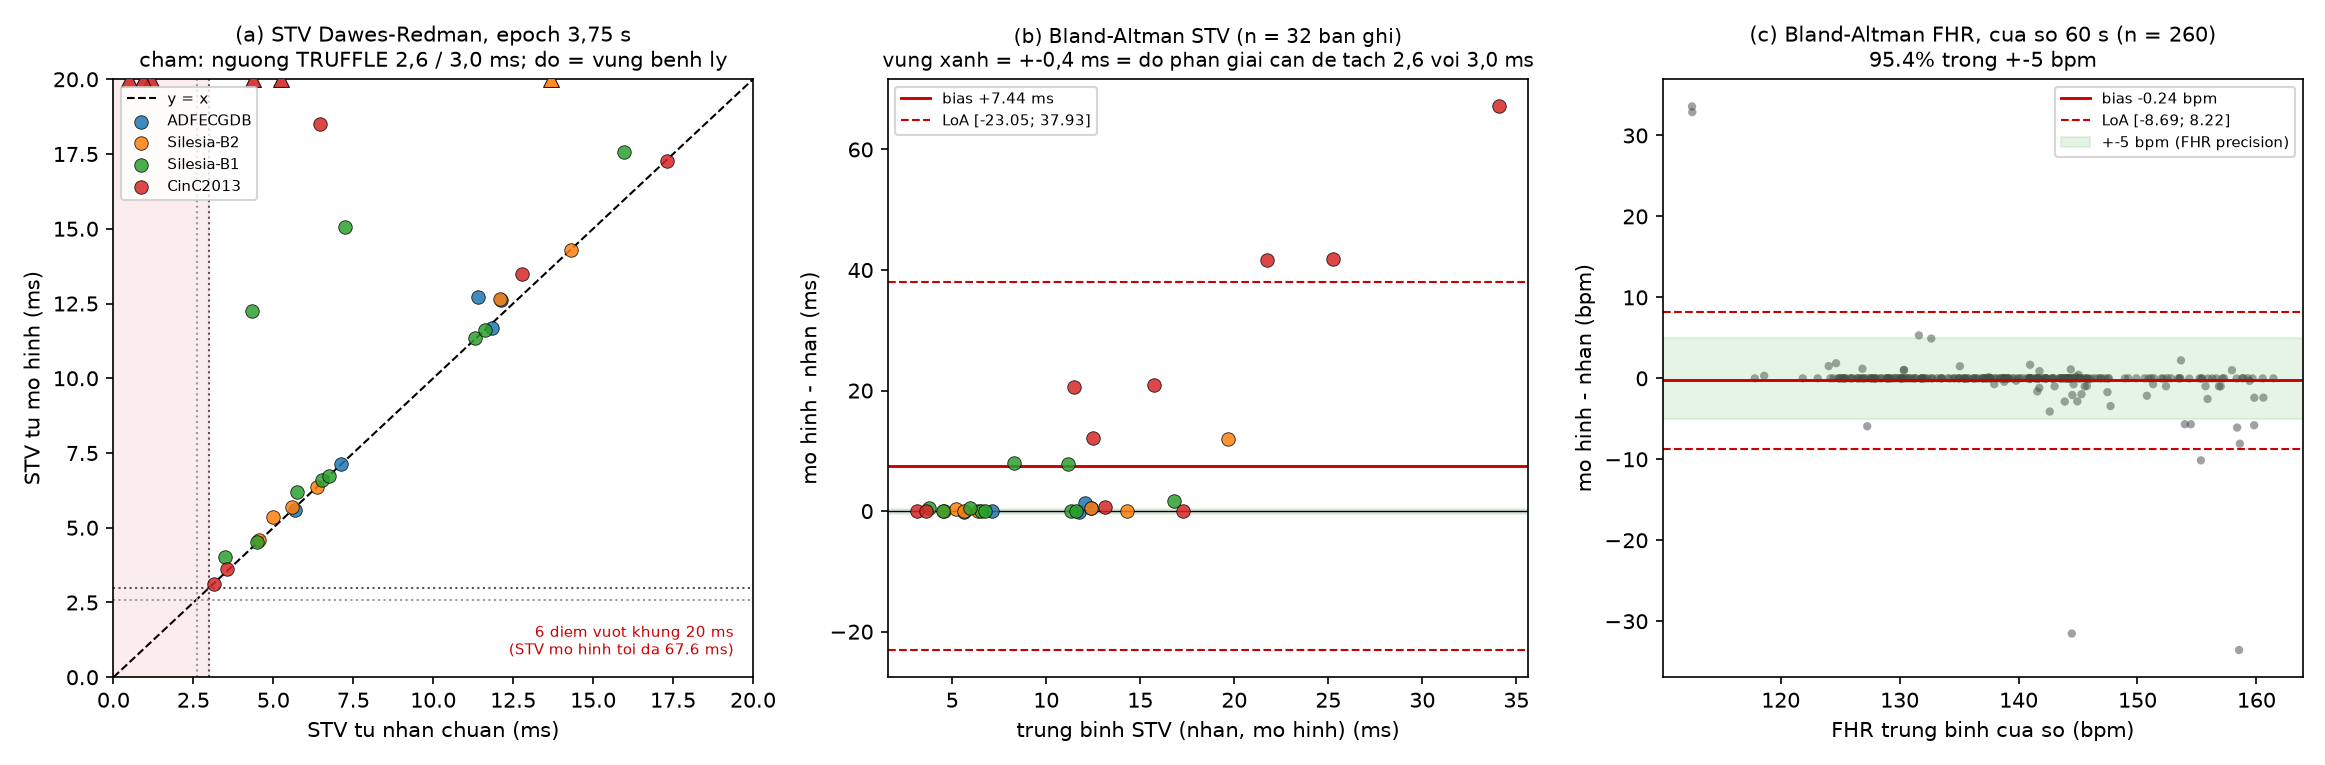
\includegraphics[width=\textwidth]{figs/clinical_stv_fhr.png}
\caption{(a) STV nhãn so với STV mô hình, phóng to vùng lâm sàng (vùng đỏ là bệnh lý). (b) Bland--Altman
cho STV. (c) Bland--Altman cho nhịp tim thai, cửa sổ 60 giây. Nguồn: \texttt{analysis/clinical.py}.}
\label{fig:clin_stv}
\end{figure}

\subsection{Nhịp tim thai --- đây là chỗ hệ thống thật sự dùng được}

\begin{table}[H]\centering\small
\caption{Bland--Altman nhịp tim thai, cửa sổ 1 phút. Mẫu số là số cửa sổ nhãn hợp lệ; 260/260 cửa sổ đều
ghép cặp được, không cửa sổ nào bị loại vì mô hình không tính nổi.}
\label{tab:fhr}
\begin{tabular}{@{}L{3.4cm} C{1.6cm} C{1.8cm} C{3.0cm} C{1.4cm} C{2.6cm}@{}}
\toprule
\textbf{Tập} & \textbf{$n$ cửa sổ} & \textbf{Độ chệch} & \textbf{LoA 95\%} & \textbf{MAE} &
\textbf{\% trong $\pm5$ bpm} \\
\midrule
ADFECGDB & 25 & $+0{,}11$ & $[-0{,}62;\ +0{,}83]$ & 0,14 & \tot{100,00} \\
Silesia B2 & 35 & $-0{,}41$ & $[-3{,}74;\ +2{,}91]$ & 0,61 & 91,43 \\
Silesia B1 & 190 & $+0{,}15$ & $[-6{,}88;\ +7{,}18]$ & 0,70 & 97,37 \\
CinC 2013 (PSD) & 10 & $-7{,}81$ & $[-34{,}60;\ +18{,}99]$ & 9,00 & \xau{60,00} \\
\midrule
\textbf{Tất cả} & 260 & $-0{,}24$ & $[-8{,}69;\ +8{,}22]$ & 0,95 & \textbf{95,38} \\
\bottomrule
\end{tabular}
\end{table}

Độ chệch ổn định ở $-0{,}23$\,bpm ở mọi độ dài cửa sổ: \textbf{không có sai lệch hệ thống về nhịp};
toàn bộ bề rộng LoA là do các bản ghi hỏng, không do sai số phân bố đều.

\begin{table}[H]\centering\small
\caption{Quét độ dài cửa sổ. Bài DPSS không nêu độ dài cửa sổ dùng cho ``FHR precision 88,61\,\%'';
cửa sổ càng dài càng dễ, nên nhóm quét cả dải. Giá trị là \% cửa sổ trong $\pm5$\,bpm.}
\label{tab:fhr_quet}
\begin{tabular}{@{}L{3.6cm} C{2.4cm} C{2.4cm} C{2.4cm} C{2.4cm}@{}}
\toprule
\textbf{Tập} & \textbf{5\,s} & \textbf{10\,s} & \textbf{30\,s} & \textbf{60\,s} \\
\midrule
ADFECGDB & \tot{98,66} ($n$=299) & \tot{98,66} ($n$=149) & 100,00 ($n$=50) & 100,00 ($n$=25) \\
Silesia B2 & 94,99 ($n$=419) & 94,26 ($n$=209) & 92,86 ($n$=70) & 91,43 ($n$=35) \\
Silesia B1 & 95,98 ($n$=2389) & 95,63 ($n$=1190) & 97,44 ($n$=390) & 97,37 ($n$=190) \\
CinC 2013 & 55,00 ($n$=120) & 51,67 ($n$=60) & 60,00 ($n$=20) & 60,00 ($n$=10) \\
\midrule
\textbf{Tất cả} & 94,58 ($n$=3227) & 94,09 ($n$=1608) & 95,66 ($n$=530) & 95,38 ($n$=260) \\
\bottomrule
\end{tabular}
\end{table}

Trên ADFECGDB, \textbf{ngay ở cửa sổ khắt khe nhất đã thử (5 giây) vẫn đạt 98,66\,\%}, cao hơn 88,61\,\%
của DPSS. Đây là so sánh \textbf{bảo vệ được}: không thể nói nhóm thắng nhờ chọn cửa sổ dài. Vẫn phải
kèm ba điều kiện: (i) DPSS chạy zero-shot từ FECGSYNDB tổng hợp còn đây là tách bản ghi trong miền ---
\textbf{hai giao thức khác nhau}; (ii) nhóm chưa chạy lại DPSS, đây là so với con số đã công bố;
(iii) $n = 5$ sản phụ.

\subsection{Độ phủ theo THỜI LƯỢNG, không theo bản ghi}

\begin{canhbao}[title={Một cách gọi tên sai phải sửa}]
Con số 43,8\,\% trong \texttt{facts\_phase2.json} và trong bản v3.2 là \textbf{tỉ lệ BẢN GHI được chấm
xanh}, \textbf{không} phải độ phủ thời gian. Hai đại lượng khác nhau và đang bị dùng lẫn. Từ đây mọi
tuyên bố về độ phủ đều là \textbf{\% thời lượng}.
\end{canhbao}

Ba chính sách khai báo trước: \textbf{P1} trả lời trừ đoạn đỏ; \textbf{P2} chỉ trả lời đoạn xanh;
\textbf{P3} như P1 nhưng bỏ cả bản ghi nếu độ tin cậy mức bản ghi là thấp.

\begin{table}[H]\centering\small
\caption{Độ phủ theo thời lượng và --- quan trọng hơn --- độ dài khoảng trống liên tục.}
\label{tab:phu}
\begin{tabular}{@{}L{2.8cm} C{1.6cm} C{1.5cm} C{1.3cm} C{1.3cm} C{1.7cm} C{3.4cm}@{}}
\toprule
\textbf{Tập} & \textbf{Thời lượng} & \textbf{Đoạn 4\,s} & \textbf{P1} & \textbf{P2} & \textbf{P3} &
\textbf{Khoảng trống P1: TV / p90 / max} \\
\midrule
ADFECGDB & 25,0 phút & 375 & \tot{96,0} & 88,8 & 96,0 & 4\,s / 12\,s / \textbf{12\,s} \\
Silesia B2 & 35,0 phút & 525 & 88,2 & 61,3 & 81,0 & 4\,s / 12\,s / \textbf{56\,s} \\
Silesia B1 & 199,6 phút & 2990 & 88,8 & 58,8 & 75,8 & 4\,s / 12\,s / \xau{192\,s} \\
CinC 2013 & 10,0 phút & 150 & \xau{58,7} & 42,7 & 39,3 & 8\,s / 33\,s / 48\,s \\
\midrule
\textbf{Tất cả} & \textbf{269,6 phút} & 4040 & \textbf{88,2} & 61,3 & 68,7 & 4\,s / 16\,s / \xau{192\,s} \\
\bottomrule
\end{tabular}
\end{table}

\begin{table}[H]\centering\small
\caption{Đối chiếu với chuẩn lâm sàng. \textbf{Các mốc CTG dưới đây do phản biện cung cấp và nhóm CHƯA
đối chiếu bản gốc} --- phải kiểm chứng trước khi đưa vào bài báo.}
\label{tab:phu_chuan}
\begin{tabular}{@{}L{5.4cm} C{2.6cm} L{6.4cm}@{}}
\toprule
\textbf{Chuẩn} & \textbf{Mất tín hiệu} & \textbf{\hethong{} tương ứng} \\
\midrule
CTG Doppler giai đoạn I & 5--8\,\% & ADFECGDB \tot{4,0\,\%} đạt; Silesia 11,2--11,8\,\% \xau{chưa đạt};
CinC 41,3\,\% \xau{chưa đạt} \\
CTG Doppler giai đoạn II & 9--20\,\% & Silesia nằm trong dải này \\
fECG bụng thương mại & 5,3\,\% & chỉ ADFECGDB đạt \\
``Mất tín hiệu cao'' & $> 20$\,\% & chỉ CinC vượt \\
\bottomrule
\end{tabular}
\end{table}

\begin{canhbao}[title={Tổng phần trăm không phải con số quan trọng nhất --- độ dài khoảng trống mới là}]
Trung vị khoảng trống là 4 giây (một đoạn đơn lẻ), vô hại. Đuôi phân bố mới là chỗ nguy hiểm:
\textbf{p90 $= 16$ giây, max $= 192$ giây} (B1\_07), và 48--64 giây ở B1\_06, B1\_10, B2\_03.

Nhịp giảm muộn kéo dài 30--90 giây; nhịp giảm kéo dài theo định nghĩa là 2--10 phút.
\textbf{Một khoảng trống 192 giây có thể giấu trọn một cơn giảm kéo dài mà máy không hề báo.}
Ở chính sách P2 (chỉ tin đoạn xanh) khoảng trống lớn nhất là \textbf{528 giây}, không thể chấp nhận
trên lâm sàng. Vì vậy mọi tuyên bố về độ phủ trong bài báo \textbf{bắt buộc} kèm p90 và max của khoảng
trống.
\end{canhbao}

Độ phủ chỉ 88,2\,\% \textbf{vì} cổng từ chối đang làm việc của nó. Nếu tắt cổng, máy trả lời 100\,\%
thời lượng nhưng 9/32 bản ghi sẽ trả kết quả sai (F1 từ 19,35 đến 89,45). Đây là một \textbf{đánh đổi}
và phải trình bày như đánh đổi, không được trình bày 88,2\,\% như khuyết điểm thuần tuý hay 100\,\%
như ưu điểm.

\begin{table}[H]\centering\small
\caption{Cổng từ chối có phân tầng đúng không.}
\label{tab:cong_tang}
\begin{tabular}{@{}L{2.8cm} C{0.9cm} C{1.6cm} C{1.6cm} C{2.4cm} C{2.4cm}@{}}
\toprule
\textbf{Mức cổng} & $n$ & \textbf{F1 TB} & \textbf{F1 min} & \textbf{$|\Delta$STV$|$ TB} &
\textbf{$|\Delta$STV$|$ max} \\
\midrule
cao & 15 & 99,92 & 99,61 & 0,15\,ms & 0,71\,ms \\
trung bình & 8 & 98,81 & 96,54 & 0,56\,ms & 1,61\,ms \\
thấp & 9 & 61,03 & 19,35 & 25,78\,ms & 67,14\,ms \\
\bottomrule
\end{tabular}
\end{table}

\textbf{Lỗi nguy hiểm theo F1 (cổng nói cao/trung bình nhưng F1 $< 90$): 0/32} --- phân tầng sạch.
\textbf{Nhưng lỗi nguy hiểm theo STV: 2} --- r10 ($+1{,}34$\,ms) và B1\_10 ($+1{,}61$\,ms), cả hai đều có
F1 $\geq 96{,}5$. Nghĩa là một cổng hiệu chuẩn cho \textit{việc dò nhịp} vẫn để lọt sai số STV đủ lớn để
lật một quyết định lâm sàng. Nếu muốn xuất STV thì phải hiệu chuẩn lại cổng theo tiêu chí STV.

\subsection{Khoá nhầm nhịp mẹ --- chế độ hỏng nguy hiểm nhất}

Nếu nhịp thai và nhịp mẹ độc lập, tỉ lệ trùng kỳ vọng là $2 \times 50\,\text{ms} / \text{RR}_{\text{mẹ}}$.
Với RR mẹ 0,46--0,77\,s trên 32 bản ghi, ngưỡng ngẫu nhiên này là \textbf{13,0--21,9\,\%}. Ước lượng giải
tích khớp sát mô phỏng dịch vòng tròn 200 lần (a02: giải tích 21,9\,\% so với mô phỏng 21,2\,\%).

\begin{ghichu}[title={Điểm phương pháp nhóm thêm vào}]
\textbf{Ngưỡng ngẫu nhiên KHÔNG phải mốc so đúng}, vì nhãn chuẩn cũng trùng đỉnh R mẹ đúng ở mức nền đó.
Mốc đúng là \textbf{chính nhãn chuẩn của bản ghi đó} --- nó hấp thụ mọi ghép cặp tần số thật giữa mẹ và
thai. Nếu chỉ so với ngưỡng ngẫu nhiên sẽ báo động giả ở 6/32 bản ghi (r01, r08, a05, a08, B2\_03,
B1\_06) mà nhãn chuẩn của chúng cũng vượt gần y hệt (r08: mô hình 20,4\,\% / nhãn 20,1\,\%; a08:
25,0\,\% / 25,0\,\%).
\end{ghichu}

\begin{table}[H]\centering\small
\caption{Khoá nhịp mẹ, so với chính nhãn chuẩn của từng bản ghi.}
\label{tab:khoame}
\begin{tabular}{@{}L{3.0cm} C{2.4cm} C{2.4cm} C{2.2cm} C{2.2cm} C{2.0cm}@{}}
\toprule
\textbf{Tập} & \textbf{Khoá mô hình} & \textbf{Khoá nhãn} & \textbf{Vượt TB} & \textbf{Vượt max} &
\textbf{Vượt $>10$ điểm} \\
\midrule
ADFECGDB & 15,7\,\% & 15,7\,\% & $-0{,}02$ & $+0{,}57$ & 0 \\
Silesia B2 & 15,0\,\% & 14,2\,\% & $+0{,}85$ & $+6{,}17$ & 0 \\
Silesia B1 & 15,9\,\% & 15,7\,\% & $+0{,}14$ & $+1{,}96$ & 0 \\
CinC 2013 & 27,4\,\% & 16,6\,\% & $+10{,}79$ & $+58{,}29$ & \xau{2} \\
\midrule
\textbf{Tất cả} & 19,3\,\% & 15,7\,\% & $+3{,}60$ & $+58{,}29$ & \xau{2} \\
\bottomrule
\end{tabular}
\end{table}

Trung vị trị tuyệt đối mức vượt trên 32 bản ghi là \textbf{0,32 điểm}: ở đại đa số bản ghi, mô hình trùng
nhịp mẹ \textbf{đúng bằng} mức mà nhãn thật cũng trùng --- không có hiện tượng bám mẹ. Chỉ hai bản ghi
thật sự khoá nhầm, cả hai đều ở CinC 2013:

\begin{table}[H]\centering\small
\caption{Hai bản ghi khoá nhầm nhịp mẹ.}
\label{tab:khoame2}
\begin{tabular}{@{}C{1.4cm} C{1.8cm} C{1.6cm} C{2.0cm} C{1.6cm} C{1.2cm} L{3.6cm}@{}}
\toprule
\textbf{Bản ghi} & \textbf{Mô hình} & \textbf{Nhãn} & \textbf{p95 rỗng} & \textbf{Vượt} & \textbf{F1} &
\textbf{Cổng gắn cờ?} \\
\midrule
a02 & \xau{78,3\,\%} & 20,0\,\% & 44,2\,\% & $+58{,}3$ & 24,91 & thấp --- luật khoá mẹ kích hoạt \\
a09 & \xau{53,4\,\%} & 15,4\,\% & 24,6\,\% & $+38{,}0$ & 19,35 & thấp --- \textbf{nhưng qua $p_{bad}$,
KHÔNG qua luật khoá mẹ} \\
\bottomrule
\end{tabular}
\end{table}

\begin{canhbao}[title={a09 là bài học quan trọng nhất của mục này}]
Hơn một nửa số ``nhịp thai'' mà mô hình trả về thực chất là nhịp mẹ, nhưng 53,4\,\% \textbf{nằm dưới
ngưỡng cứng 60\,\%} nên luật ghi đè khoá mẹ \textbf{không kích hoạt}. Bản ghi được cứu là nhờ điểm
$p_{bad}$ của bộ phân loại SQI --- \textbf{may, không phải thiết kế}.

\textbf{Khuyến nghị cụ thể, rẻ và nên làm ngay:} thay luật ngưỡng tuyệt đối 60\,\% bằng \textbf{mức vượt
so với phân phối rỗng của chính bản ghi}. Cắt ở ``vượt p95 mô phỏng hơn 10 điểm'' bắt đúng cả a02 lẫn
a09 và không tạo dương tính giả nào trong 30 bản ghi còn lại.
\end{canhbao}

\begin{figure}[H]\centering
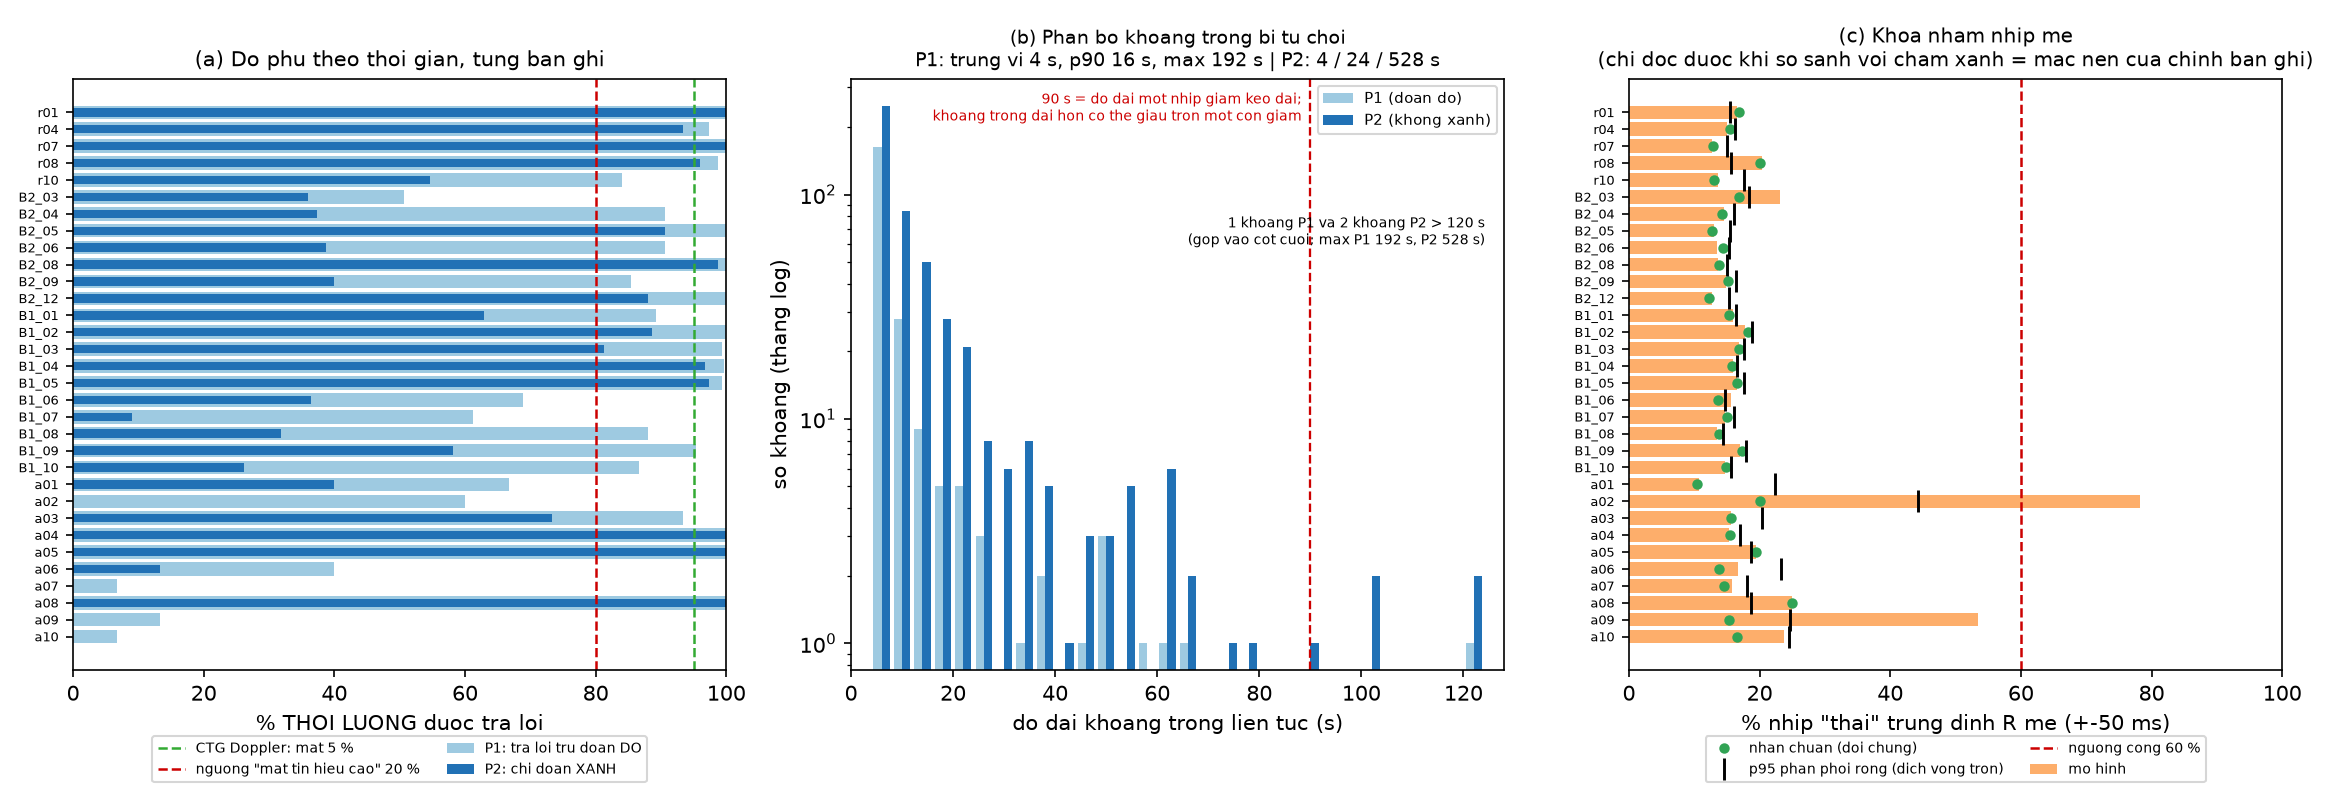
\includegraphics[width=\textwidth]{figs/clinical_coverage_lock.png}
\caption{(a) \% thời lượng trả lời từng bản ghi so với mốc CTG. (b) Phân bố độ dài khoảng trống, thang
log, mốc 90 giây. (c) Khoá nhịp mẹ so với nhãn chuẩn và phân phối rỗng.}
\label{fig:clin_cov}
\end{figure}

\subsection{Chọn kênh sửa được F1, nhưng không sửa được STV}

\begin{table}[H]\centering\small
\caption{Bốn bản ghi CinC 2013 kém nhất: quy tắc PSD mù nhãn so với kênh 0 hậu kiểm. STV tính bằng ms.}
\label{tab:clin_kenh}
\begin{tabular}{@{}C{1.6cm} C{3.6cm} C{3.6cm} C{2.2cm}@{}}
\toprule
\textbf{Bản ghi} & \textbf{PSD: F1 / STV / phủ} & \textbf{Kênh 0: F1 / STV / phủ} & \textbf{STV nhãn} \\
\midrule
a01 & 80,99 / 18,52 / 66,7\,\% & 100,00 / 6,53 / 86,7\,\% & 6,45 \\
a07 & 45,63 / 42,57 / 6,7\,\% & 86,92 / 12,47 / 80,0\,\% & 0,93 \\
a09 & 19,35 / 67,63 / 13,3\,\% & 94,25 / 6,37 / 93,3\,\% & 0,49 \\
a10 & 47,13 / 46,16 / 6,7\,\% & 70,89 / 27,58 / 46,7\,\% & 4,37 \\
\bottomrule
\end{tabular}
\end{table}

Điều đáng chú ý về lâm sàng: \textbf{ngay cả ở kênh 0 với F1 $= 94{,}25$, STV của a09 vẫn là 6,37\,ms so
với nhãn 0,49\,ms --- sai 13 lần}. Vấn đề STV \textbf{không} sửa được bằng cách chọn kênh tốt hơn. Chọn
kênh sửa được F1 và độ phủ; nó không sửa được độ phân giải STV.

\subsection{Những gì mục này KHÔNG chứng minh được}

\begin{enumerate}[leftmargin=1.6em,itemsep=3pt]
\item \textbf{Không có dữ liệu trong vùng ra quyết định.} 22 chủ thể trong miền có STV nhãn 3,49--15,97\,ms;
không ai gần 2,6--3,0\,ms. Không thể ước lượng độ nhạy / độ đặc hiệu của cờ ``STV thấp''.
\item \textbf{22/32 bản ghi ngắn hơn tối thiểu 10 phút của Dawes--Redman} (ADFECGDB và B2 là 5 phút, CinC
là 1 phút). Chỉ 10 bản B1 cho một trị số STV hợp lệ về thời lượng.
\item \textbf{Không có thai dưới 38 tuần trong ADFECGDB}, trong khi giá trị lâm sàng của STV nằm ở tuần
24--37.
\item \textbf{Ngưỡng TRUFFLE 2,6 / 3,0\,ms và các mốc mất tín hiệu CTG đều chưa được nhóm đối chiếu bản
gốc.} Phải kiểm chứng và trích dẫn đúng trước khi đưa vào bài báo.
\item \textbf{STV Dawes--Redman gốc tính trên tín hiệu CTG Doppler lấy mẫu đều}, không phải trên chuỗi RR
từng nhịp. Định nghĩa dùng ở đây là bản thích ứng hợp lý cho fECG nhưng \textbf{không đồng nhất} với
thuật toán gốc.
\item \textbf{Một seed, một fold cho mỗi chủ thể.} B2\_03 --- bản ghi có sai số STV lớn nhất trong miền
($+11{,}99$\,ms) --- cũng chính là bản ghi kém ổn định nhất theo seed ($|$hiệu$|$ 2,81 điểm F1, xem
\S\ref{sec:thongke}). Sai số STV của nó có thể phần lớn là nhiễu huấn luyện.
\item Các hệ số tương quan ở bảng \ref{tab:stv} ($r = 0{,}986$ với $n = 5$) là \textbf{mô tả}, không được
trình bày như bằng chứng thống kê.
\end{enumerate}

\begin{ghichu}[title={Phát biểu cuối cùng về giá trị lâm sàng}]
\hethong{} hiện là \textbf{một bộ đếm nhịp tim thai tốt, không phải một máy đo biến thiên}.
Nhịp tim thai: sai số trung bình dưới 1\,bpm, 95,38\,\% cửa sổ trong $\pm5$\,bpm trên 260 cửa sổ, và
98,66\,\% ngay ở cửa sổ 5 giây trên ADFECGDB --- \textbf{dùng được}.
STV: độ phân giải thiếu 2,5--4,5 lần, sai số một chiều về phía trấn an giả, 3/3 bản ghi tham chiếu thấp
nhất bị bỏ sót --- \textbf{chưa dùng được, và nhóm nói thẳng điều đó thay vì im lặng}.
Độ phủ: đạt chuẩn CTG trên ADFECGDB, chưa đạt trên Silesia, hỏng trên CinC --- và khoảng trống 192 giây
là con số phải sửa trước khi nói đến thử nghiệm lâm sàng.
\end{ghichu}

\clearpage
% ================================================================= THỐNG KÊ Ở MỨC CHỦ THỂ
\section{Kiểm định lại toàn bộ thống kê ở mức chủ thể}
\label{sec:thongke}

Mục này sửa một lỗi phương pháp có mặt trong \textbf{mọi} bản đề cương trước và trong bản thảo hội nghị:
đơn vị phân tích. Mã tại \texttt{analysis/stats.py}, kết quả tại \texttt{analysis/stats\_results.json} và
\texttt{analysis/STATS.md}. Bootstrap cụm 10.000 lần, seed 0; biên tương đương khai báo trước
$\delta = 1{,}0$ điểm F1.

\subsection{Lỗi đã sửa}

\begin{table}[H]\centering\small
\caption{Sáu thay đổi phương pháp.}
\label{tab:stat_sua}
\begin{tabular}{@{}L{3.4cm} L{5.2cm} L{5.6cm}@{}}
\toprule
 & \textbf{Cách cũ} & \textbf{Cách mới} \\
\midrule
Đơn vị phân tích & Cặp (bản ghi $\times$ kênh), 20--88 cặp & \textbf{Chủ thể} (trung bình 4 kênh trước),
$n = 5$--22 \\
Giả định độc lập & 4 kênh bụng của cùng một phụ nữ coi là 4 quan sát độc lập & Kênh là đo lặp lại trong
cụm; chủ thể là đơn vị \\
Khoảng tin cậy & $t$ trên thang phần trăm & Thang logit $+$ bootstrap percentile \\
Biến thiên & SD trên cặp & Bootstrap cụm, lấy mẫu lại \textbf{chủ thể} \\
Đa so sánh & không hiệu chỉnh & Holm cho họ 7 kiến trúc \\
Kết luận ``không khác'' & $p > 0{,}05$ & \textbf{TOST} biên 1,0 điểm \\
\bottomrule
\end{tabular}
\end{table}

\begin{canhbao}[title={Giới hạn cứng của $n = 5$ --- con số phải ghi nhớ}]
Với $n = 5$ chủ thể, kiểm định Wilcoxon hạng có dấu hai phía có $p$ \textbf{nhỏ nhất có thể đạt} là
$2/2^5 = \mathbf{0{,}0625}$. Do đó \textbf{KHÔNG một so sánh nào} trên ADFECGDB (5 sản phụ) có thể đạt
$p < 0{,}05$ ở mức chủ thể, bất kể hiệu số lớn đến đâu.

Mọi $p < 0{,}05$ từng báo cáo trên tập này --- $1{,}9\times10^{-6}$, $5{,}7\times10^{-6}$, $0{,}0000$ ---
đều là \textbf{sản phẩm của giả lập} (pseudo-replication) trên 20--60 hàng (bản ghi $\times$ kênh
$\times$ seed). Chúng đã bị gỡ khỏi toàn bộ đề cương.
\end{canhbao}

\subsection{Bảng tổng hợp: mọi so sánh chính, tính lại ở mức chủ thể}

\begin{table}[H]\centering\scriptsize
\caption{Quy ước hiệu số: \textbf{A $-$ B} với A là đối tượng đứng đầu trong tên so sánh. Cột ``KTC 95\%
$t$'' bảo thủ hơn; khi hai cột mâu thuẫn thì tin cột $t$.}
\label{tab:stat_all}
\begin{tabular}{@{}L{4.4cm} C{0.5cm} C{1.5cm} C{1.3cm} C{1.1cm} C{2.0cm} C{2.0cm} C{0.9cm}@{}}
\toprule
\textbf{So sánh} & $n$ & \textbf{$p$ cũ (giả lập)} & \textbf{$p$ mới} & \textbf{Hiệu số} &
\textbf{KTC 95\% bootstrap} & \textbf{KTC 95\% $t$} & \textbf{Cliff} \\
\midrule
\multicolumn{8}{@{}l}{\textit{ADFECGDB, trung bình 4 kênh --- mô hình so với baseline cổ điển:}} \\
vs TS & 5 & $5{,}7\times10^{-6}$ & \xau{0,0625} & $+18{,}49$ & $[+6{,}38; +30{,}60]$ &
\xau{$[-1{,}81; +38{,}80]$} & 1,000 \\
vs TS-PCA & 5 & $1{,}9\times10^{-6}$ & \xau{0,0625} & $+6{,}40$ & $[+4{,}70; +8{,}09]$ &
\tot{$[+3{,}69; +9{,}10]$} & 0,920 \\
vs Prominence & 5 & $1{,}9\times10^{-6}$ & \xau{0,0625} & $+11{,}06$ & $[+7{,}80; +14{,}51]$ &
\tot{$[+5{,}73; +16{,}38]$} & 1,000 \\
\midrule
\multicolumn{8}{@{}l}{\textit{Mô hình 22 ca so với mô hình 5 ca, trung bình 4 kênh:}} \\
PhysioNet & 5 & 0,2445 & 0,8125 & $+1{,}24$ & $[-0{,}35; +3{,}01]$ & $[-1{,}44; +3{,}91]$ & 0,200 \\
Silesia B2 & 7 & \xau{0,0156} & \xau{0,4688} & $+0{,}77$ & $[-0{,}16; +2{,}38]$ & $[-1{,}15; +2{,}68]$ & 0,102 \\
Silesia B1 & 10 & $4{,}3\times10^{-9}$ & 0,0039 & $+5{,}71$ & $[+2{,}12; +10{,}17]$ &
$[+0{,}79; +10{,}62]$ & 0,500 \\
Toàn bộ 22 & 22 & $1{,}5\times10^{-8}$ & 0,0029 & $+3{,}12$ & $[+1{,}27; +5{,}48]$ &
$[+0{,}76; +5{,}48]$ & 0,264 \\
\midrule
\multicolumn{8}{@{}l}{\textit{Tầng 2 (ngữ cảnh) --- TCN trường 1.516\,ms so với CNN cửa sổ ngắn:}} \\
Tăng do ngữ cảnh & 5 & --- & 0,0625 & $+4{,}49$ & $[+1{,}58; +7{,}43]$ & \xau{$[-0{,}29; +9{,}27]$} & 0,520 \\
\bottomrule
\end{tabular}
\end{table}

\begin{ghichu}[title={Ba điều phải đọc kèm bảng trên}]
\begin{enumerate}[leftmargin=1.5em,itemsep=4pt]
\item \textbf{Mất ý nghĩa không tự động có nghĩa là mất hiệu ứng --- nhưng với TS thì mất thật.}
Với TS-PCA và Prominence, $p$ tăng từ $\sim10^{-6}$ lên 0,0625 chỉ vì $n = 5$ làm sàn kiểm định hạng,
còn KTC 95\% của hiệu số vẫn \textbf{loại trừ 0} ở cả bootstrap lẫn thang $t$. Với hai baseline này,
\textit{hướng} của kết quả giữ nguyên; chỉ là \textbf{không được tuyên bố ý nghĩa thống kê} từ 5 phụ nữ.
Nhưng với \textbf{TS thì khác}: KTC 95\% kiểu $t$ là $[-1{,}81;\ +38{,}80]$ --- \textbf{chứa cả 0}. Hiệu
số 18,49 điểm hoàn toàn do biến thiên giữa 5 bản ghi. Bảng baseline cũ trình bày cả ba như nhau; thực tế
chúng không cùng độ chắc.
\item \textbf{Bootstrap với $n = 5$ cụm hẹp hơn thực tế.} Với $n = 5$--7 phải báo cáo cả hai cột.
\item \textbf{Sign test bảo thủ nhất và cho thấy độ mạnh thật.} Ví dụ ``toàn bộ 22 chủ thể'' có Wilcoxon
$p = 0{,}0029$ nhưng sign test $p = 0{,}0525$ --- kết quả phụ thuộc vào \textbf{độ lớn} của vài chủ thể,
không phải vào việc đa số chủ thể đều cải thiện.
\end{enumerate}
\end{ghichu}

\subsection{Khoảng tin cậy cho các con số đặt trên tiêu đề}

\begin{table}[H]\centering\small
\caption{Cột ``KTC 95\% $t$ trên \%'' là cột \textbf{đang có lỗi} trong các bản trước: nó \textbf{vượt
100\%}. Cột in đậm là cột phải dùng trong bảng kết quả chính.}
\label{tab:stat_ktc}
\begin{tabular}{@{}L{5.4cm} C{0.7cm} C{1.4cm} C{2.6cm} C{2.8cm} C{2.4cm}@{}}
\toprule
\textbf{Con số} & $n$ & \textbf{TB} & \textbf{KTC 95\% $t$ trên \% (SAI)} &
\textbf{KTC 95\% bootstrap} & \textbf{KTC 95\% logit} \\
\midrule
ADFECGDB kênh PSD, mô hình 5 ca & 5 & 99,21 & \xau{$[97{,}35; 101{,}08]$} &
\textbf{$[97{,}87; 99{,}95]$} & $[98{,}21; 99{,}96]$ \\
ADFECGDB 4 kênh, mô hình 5 ca & 5 & 97,45 & \xau{$[93{,}77; 101{,}13]$} &
\textbf{$[94{,}94; 99{,}63]$} & $[90{,}65; 99{,}90]$ \\
Silesia B1, mô hình 5 ca & 10 & 93,30 & \xau{$[83{,}67; 102{,}93]$} &
\textbf{$[84{,}93; 99{,}37]$} & $[94{,}79; 99{,}72]$ \\
Silesia B1, mô hình 22 ca & 10 & 97,15 & \xau{$[93{,}61; 100{,}69]$} &
\textbf{$[94{,}00; 99{,}67]$} & $[97{,}85; 99{,}93]$ \\
\bottomrule
\end{tabular}
\end{table}

\begin{canhbao}[title={Hai ước lượng điểm khác nhau, dùng nhầm là sai}]
Cột \textbf{bootstrap} là khoảng cho \textbf{trung bình số học} của F1 trên các chủ thể --- đây là đại
lượng mà đề cương đang báo cáo (99,21 / 93,30). Nó không bao giờ vượt 100\% vì chỉ lấy lại mẫu từ các
giá trị quan sát. Dùng cột này trong bảng kết quả chính.

Cột \textbf{logit} là ``F1 điển hình của một chủ thể mới'', kéo về phía các giá trị cao, nên nó
\textbf{có thể cao hơn} trung bình số học (Silesia B1: TB số học 93,30 nhưng điểm logit 98,78). Dùng cột
này khi nói về \textbf{một ca lâm sàng mới}, và phải nói rõ đó là đại lượng \textbf{khác} --- nếu báo cáo
nhầm, con số sẽ bị thổi phồng.

Độ rộng thật: ADFECGDB $n = 5$ cho KTC rộng vài điểm F1 (không phải $\pm1{,}5$ như SD gợi ý); Silesia B1
và CinC 2013 rộng hơn 10--30 điểm.
\end{canhbao}

\subsection{Họ kiến trúc: kiểm định tương đương (TOST), biên 1,0 điểm F1}

\begin{table}[H]\centering\small
\caption{TOST với biên tương đương $\delta = 1{,}0$ điểm F1, $n = 5$ chủ thể, hiệu chỉnh Holm cho họ
7 so sánh.}
\label{tab:tost}
\begin{tabular}{@{}L{2.0cm} C{1.7cm} C{1.6cm} C{1.5cm} C{1.5cm} C{2.6cm} C{1.2cm} L{2.2cm}@{}}
\toprule
\textbf{Kiến trúc} & \textbf{Macro F1} & \textbf{Hiệu số} & \textbf{$p$ Wilc.} & \textbf{$p$ Holm} &
\textbf{KTC 90\% bootstrap} & \textbf{$p$ TOST} & \textbf{Kết luận} \\
\midrule
\texttt{cnn\_l} & 92,43 & $+0{,}73$ & 0,125 & 0,625 & $[+0{,}18; +1{,}22]$ & 0,238 & không kết luận được \\
\texttt{mlp} & 91,64 & $-0{,}07$ & 1,000 & 1,000 & $[-3{,}47; +3{,}52]$ & 0,360 & không kết luận được \\
\texttt{cnn\_gru} & 91,59 & $-0{,}12$ & 0,813 & 1,000 & $[-0{,}72; +0{,}54]$ & 0,058 & không kết luận được \\
\texttt{tcn} & 91,07 & $-0{,}64$ & 0,188 & 0,750 & $[-1{,}13; -0{,}11]$ & 0,183 & không kết luận được \\
\texttt{resnet1d} & 90,90 & $-0{,}81$ & 0,625 & 1,000 & $[-1{,}79; +0{,}09]$ & 0,389 & không kết luận được \\
\texttt{cnn\_m} & 88,76 & $-2{,}95$ & 0,063 & 0,438 & \xau{$[-4{,}55; -1{,}47]$} & 0,930 &
\xau{KÉM HƠN vượt biên} \\
\texttt{linear} & 37,47 & $-54{,}24$ & 0,063 & 0,438 & $[-56{,}41; -50{,}49]$ & 1,000 & khác biệt vượt biên \\
\bottomrule
\end{tabular}
\end{table}

\begin{canhbao}[title={Đây là đảo chiều lớn nhất của toàn bộ đợt rà soát}]
Tuyên bố trong bản v3.2 và trong kho mã --- \textit{``tám kiến trúc không phân biệt được, không cái nào
khác \texttt{cnn\_dil} 26k tham số''} --- \textbf{không sống sót qua kiểm định tương đương}:

\begin{itemize}[leftmargin=1.5em,itemsep=3pt]
\item \textbf{0/7} kiến trúc chứng minh được tương đương trong biên $\pm1{,}0$ điểm F1;
\textbf{6/7} \textbf{không kết luận được}.
\item Kết luận cũ rút ra từ $p > 0{,}05$. Với $n = 5$ chủ thể, $p > 0{,}05$ là kết quả \textbf{gần như
đương nhiên} (ngưỡng khả thi nhỏ nhất là 0,0625) --- nó đo \textbf{công suất thấp}, không đo sự giống nhau.
\item Ngược lại, \texttt{cnn\_m} \textbf{KÉM HƠN rõ}: hiệu số $-2{,}95$ điểm, KTC 90\% bootstrap
$[-4{,}55;\ -1{,}47]$ nằm \textbf{hoàn toàn ngoài} biên $\pm1{,}0$. Tuyên bố ``sáu kiến trúc nằm trong
1,5 điểm của nhau'' không đúng với \texttt{cnn\_m}.
\item \texttt{cnn\_l} \textbf{tốt hơn} \texttt{cnn\_dil} 0,73 điểm, KTC 90\% bootstrap
$[+0{,}18;\ +1{,}22]$ --- không loại trừ được khả năng vượt biên 1,0.
\end{itemize}

\textbf{Phát biểu thay thế, là câu nhóm sẽ dùng:} \textit{``Với $n = 5$ chủ thể, nghiên cứu này
\textbf{không đủ lực} để phân biệt các kiến trúc trong biên 1,0 điểm F1; hiệu số quan sát được nằm trong
khoảng $-2{,}95$ đến $+0{,}73$ điểm, nhỏ hơn nhiều so với $+11{,}00$ điểm của tầng front-end.''}
Câu này giữ nguyên thông điệp chính (front-end quan trọng hơn kiến trúc) mà không tuyên bố điều chưa
chứng minh.
\end{canhbao}

\subsection{Cổng từ chối: AUROC trong bản ghi mới là con số lâm sàng}

\begin{table}[H]\centering\small
\caption{Cluster bootstrap theo \textbf{bản ghi} ($n = 10$ cụm), không theo đoạn.}
\label{tab:auroc}
\begin{tabular}{@{}L{6.4cm} C{2.0cm} C{3.4cm} C{2.2cm}@{}}
\toprule
\textbf{Đại lượng} & \textbf{Giá trị} & \textbf{KTC 95\% cụm} & \textbf{Báo cáo cũ} \\
\midrule
AUROC (12 SQI cổ điển, CinC 2013) & 0,929 & $[0{,}830;\ 0{,}982]$ & 0,929 \\
Lợi ích F1 ở độ phủ 80\% & 7,49 & $[2{,}94;\ 11{,}54]$ & 7,37 \\
AUROC nhóm đặc trưng tô-pô & 0,566 & chưa tính được & 0,566 \\
\midrule
\textbf{AUROC TRONG bản ghi} (TB trên 5 bản ghi có cả đoạn tốt lẫn xấu) & \textbf{0,721} &
$[0{,}517;\ 0{,}898]$ & \xau{chưa từng báo cáo} \\
\bottomrule
\end{tabular}
\end{table}

AUROC từng bản ghi: a01 $= 0{,}914$; a06 $= 0{,}390$; a07 $= 0{,}889$; a09 $= 0{,}886$; a10 $= 0{,}526$.
Năm bản ghi còn lại không có đoạn xấu nào nên không đóng góp gì vào AUROC gộp.

\begin{canhbao}[title={Phát hiện mới, quan trọng cho C3}]
AUROC gộp 0,93 \textbf{phần lớn là hiệu ứng GIỮA bản ghi} (tách bản ghi tốt khỏi bản ghi xấu), không
phải khả năng xếp hạng đoạn \textbf{BÊN TRONG} một bản ghi. Trong ứng dụng thật --- một thai phụ, một
phiên đo --- chỉ AUROC \textbf{trong} bản ghi mới có ý nghĩa, và con số đó là \textbf{0,721}
$[0{,}517;\ 0{,}898]$.

Con số 0,929 trên thực tế trả lời câu hỏi \textit{``bản ghi này có phải bản ghi xấu không''}, trong khi
cổng từ chối đang được bán như là thứ trả lời \textit{``đoạn 4 giây này trong bản ghi của bệnh nhân này
có đáng tin không''}. Đây là giới hạn phải nêu rõ, và là lý do kết quả C3 \textbf{chưa} thể tuyên bố là
dùng được tại giường bệnh.
\end{canhbao}

\subsection{Độ ổn định theo seed}

Tất cả kết quả chính chạy \textbf{một seed}. Nhóm đã huấn luyện lại toàn bộ mô hình 22 chủ thể với
seed 1 (\texttt{model/train\_22\_seed1.json}) để đo biến thiên huấn luyện.

\begin{table}[H]\centering\small
\caption{So sánh seed 0 với seed 1 trên 20 chủ thể chung, kênh PSD mù nhãn.}
\label{tab:seed}
\begin{tabular}{@{}L{7.4cm} C{3.2cm} L{4.0cm}@{}}
\toprule
\textbf{Đại lượng} & \textbf{Giá trị} & \textbf{Đọc thế nào} \\
\midrule
Số chủ thể chung & 20 & \\
$|$hiệu số$|$ F1 trung bình & \tot{0,28 điểm} & nhỏ so với mọi hiệu ứng báo cáo \\
$|$hiệu số$|$ lớn nhất & 2,81 điểm (B2\_03) & bản ghi kém ổn định nhất \\
Ngưỡng từng fold, seed 0 & 0,20 -- 0,80 & có một giá trị cực đoan 0,20 \\
Ngưỡng từng fold, seed 1 & 0,50 -- 0,80 & \xau{không tái lập giá trị 0,20} \\
\bottomrule
\end{tabular}
\end{table}

Hai kết luận. Thứ nhất, \textbf{biến thiên theo seed (0,28 điểm) nhỏ hơn nhiều so với mọi hiệu ứng được
báo cáo} trong đề cương --- $+11{,}00$ của front-end, $+4{,}49$ của ngữ cảnh, $+8{,}18$ của dữ liệu trên
CinC 75 bản ghi. Các kết luận định tính không bị seed lật. Thứ hai, \textbf{ngưỡng từng fold kém ổn định
hơn hẳn}: giá trị 0,20 của fold 10 ở seed 0 không tái lập ở seed 1 (dải 0,50--0,80). Đó là cảnh báo rằng
quy trình chọn ngưỡng trên một chủ thể validation duy nhất là điểm mong manh của pipeline.

\begin{ghichu}[title={Mọi KTC trong đề cương này bao phủ cái gì}]
Bootstrap cụm trong mục này lấy mẫu lại \textbf{chủ thể}, nên KTC bao phủ \textbf{biến thiên giữa chủ
thể}. Chúng \textbf{không} bao phủ biến thiên huấn luyện; phần đó được đo riêng ở bảng \ref{tab:seed} và
bằng 0,28 điểm trung bình.
\end{ghichu}

\subsection{Những gì KHÔNG kiểm chứng lại được từ artefact hiện có}

\begin{table}[H]\centering\small
\caption{Ba mục nhóm không thể tự kiểm chứng lại, và hệ quả.}
\label{tab:stat_khong}
\begin{tabular}{@{}L{4.0cm} L{5.4cm} L{5.0cm}@{}}
\toprule
\textbf{Mục} & \textbf{Lý do} & \textbf{Hệ quả} \\
\midrule
Tầng 1 --- front-end dải thông ($+11{,}00$ điểm, từng ghi $p < 0{,}001$) &
\texttt{pilot\_evidence/band\_ablation.json} chỉ lưu tổng hợp (macro F1 $\pm$ SD cho mỗi dải), KHÔNG lưu
F1 từng bản ghi $\times$ kênh &
\xau{$p < 0{,}001$ cho tầng 1 hiện KHÔNG kiểm chứng được.} Hiệu số $+11{,}00$ vẫn đứng; trị số $p$ đã bị
gỡ. Phải chạy lại có lưu per-record \\
AUROC nhóm đặc trưng tô-pô (0,566) & \texttt{fsqi/gate\_segments.csv} chỉ lưu $p_{bad}$ của bộ phân loại
SQI cổ điển; muốn bootstrap theo cụm phải huấn luyện lại &
0,566 vẫn dùng làm kết luận phủ định, nhưng chưa có KTC theo cụm \\
Biến thiên theo seed cho các bảng cũ & Chỉ mô hình 22 ca có 2 seed; bảng kiến trúc và khảo sát dải chỉ
1 seed & KTC hiện có chỉ bao phủ biến thiên giữa chủ thể \\
\bottomrule
\end{tabular}
\end{table}

\subsection{Nguyên tắc chung cho mọi con số từ đây}

\begin{enumerate}[leftmargin=1.6em,itemsep=3pt]
\item Báo cáo \textbf{ước lượng hiệu số kèm KTC} làm kết quả chính; $p$-value là phụ và phải luôn đi kèm
$n$ chủ thể.
\item Với $n = 5$--10, \textbf{không tuyên bố ý nghĩa thống kê ở bất kỳ đâu}.
\item Với kết luận ``không khác nhau'', \textbf{bắt buộc} dùng TOST kèm biên được định trước.
\item Đơn vị phân tích luôn là \textbf{chủ thể}; kênh là đo lặp lại trong cụm.
\item Với $n = 75$ (CinC 2013 toàn bộ) thì kiểm định \textbf{có} đủ lực và $p$ được báo cáo bình thường
--- đó là tập duy nhất trong đề tài đủ lớn cho điều đó.
\end{enumerate}

\clearpage
% ================================================================= 7. HỆ THỐNG AGENT
\section{Khảo sát ý tưởng hệ thống nhiều mô hình}
\label{sec:agent}

Một hướng nhóm cân nhắc là: thay vì một mô hình duy nhất, xây một hệ thống nhiều tác tử, mỗi nhiệm vụ
con dùng mô hình tối ưu riêng cho nó. Mục này là kết quả khảo sát nghiêm túc ý tưởng đó, dựa trên bằng
chứng từ 30 công trình đã đọc và từ số đo của chính nhóm.

\subsection{Nhận xét đầu tiên: pipeline hiện tại đã là hệ dị thể}

Pipeline của nhóm hiện gồm bốn khối dùng bốn loại công cụ khác nhau: lọc Butterworth (xử lý tín hiệu
cổ điển), mẫu trung vị kết hợp bình phương tối thiểu (thống kê cổ điển), mạng tích chập giãn nở (học sâu),
và lấy đỉnh có thời gian trơ (luật xác định). Đây \textbf{đã là} nguyên tắc ``mỗi việc một công cụ tối ưu''.
Thêm một tầng điều phối lên trên chỉ đổi tên gọi chứ không thêm năng lực.

\subsection{Phân rã bảy nhiệm vụ con và mô hình tối ưu cho từng nhiệm vụ}

\begin{table}[H]\centering\small
\caption{Bảy nhiệm vụ con của bài toán và mô hình tối ưu theo bằng chứng từ y văn cùng số đo của nhóm.}
\label{tab:nhiemvu}
\begin{tabular}{@{}C{0.8cm} L{3.4cm} L{5.0cm} L{4.6cm}@{}}
\toprule
\textbf{\#} & \textbf{Nhiệm vụ con} & \textbf{Mô hình tối ưu theo bằng chứng} & \textbf{Trạng thái} \\
\midrule
1 & Đánh giá chất lượng tín hiệu & Còn bỏ ngỏ. Heuristic phổ sụp ngoài miền (\S\ref{sec:chonkenh}) &
\xau{Đây chính là C3} \\
2 & Dò QRS mẹ & Luật cổ điển kiểu Pan--Tompkins & Đã có, đủ tốt \\
3 & Khử ECG mẹ & \textbf{Còn tranh chấp thật}: trừ mẫu, lọc Kalman mở rộng, hay mạng tái tạo &
Cơ hội cải tiến \\
4 & Dò QRS thai & Đã bão hoà: đổi kiến trúc chỉ $+0{,}41$ điểm, $p = 0{,}7012$ & Đã có, khó cải thiện \\
5 & Sửa lỗi nhịp, nội suy khoảng mất & Làm mượt khoảng RR bằng luật sinh lý & Chưa làm \\
6 & Ước lượng nhịp tim thai & Tính trực tiếp từ khoảng RR & Đã có \\
7 & Quyết định từ chối trả lời & Chưa có tiền lệ cho tín hiệu thai & \xau{Đây chính là C3} \\
\bottomrule
\end{tabular}
\end{table}

Trong bảy nhiệm vụ, \textbf{năm} có lời giải tốt nhất là giải pháp cổ điển xác định, \textbf{một} đã bão
hoà, và chỉ \textbf{một} (khử ECG mẹ) còn tranh chấp thật sự về mô hình.

\subsection{Y văn nói gì về hướng nhiều mô hình}

Trong 30 công trình đã đọc, \textbf{không có công trình nào} dùng tác tử ngôn ngữ lớn hoặc kiến trúc
hỗn hợp chuyên gia có cổng học được cho bài toán điện tim thai. Nhưng \textbf{có} tiền lệ rõ ràng cho
hợp nhất và nối tầng:

\begin{table}[H]\centering\small
\caption{Tiền lệ hợp nhất và nối tầng trong y văn, kèm mức lợi ích công bố.}
\label{tab:ensemble}
\begin{tabular}{@{}L{5.4cm} L{4.4cm} L{4.6cm}@{}}
\toprule
\textbf{Công trình} & \textbf{Cơ chế} & \textbf{Mức lợi ích công bố} \\
\midrule
Behar và cộng sự 2014 (FUSE) & Hợp nhất nhiều bộ trích xuất & khoảng $+3{,}0$ điểm F1 so với phương
pháp đơn tốt nhất \\
Shokouhmand \& Tavassolian 2023 & Nối tầng khối khử nhiễu trước tách nguồn & $+22{,}45$ điểm \\
Asadi và cộng sự 2025 & Nối tầng hai mạng U-Net & $+1{,}1$ đến $+1{,}6$ điểm độ nhạy \\
Behar và cộng sự 2014 (cổng bSQI) & \textbf{Cổng từ chối} theo chất lượng & $+0{,}95$ đến $+1{,}11$ điểm
khi chỉ loại 3,6\% tín hiệu \\
\bottomrule
\end{tabular}
\end{table}

\begin{ghichu}[title={Kết luận quan trọng nhất của mục này}]
Giá trị của ``tác tử'' trong y văn điện tim thai nằm ở \textbf{quyền chọn} và \textbf{quyền từ chối},
không nằm ở việc luân chuyển giữa nhiều mô hình dò. Điều này trùng khít với đóng góp C3 mà nhóm đã đề xuất.
\end{ghichu}

\subsection{Còn bao nhiêu dư địa để cải tiến}

Trong miền, nhóm đang ở 99,21 (kênh mù nhãn) và 97,45 (trung bình bốn kênh). Trần là 100. Nghĩa là dư địa
còn lại chỉ \textbf{0,79} đến \textbf{2,55} điểm. Trong khi đó, ngưỡng phân giải thống kê thực nghiệm của
nhóm nằm đâu đó giữa 0,41 điểm (không phân biệt được, $p = 0{,}70$) và 4,53 điểm (phân biệt rõ,
$p = 0{,}0000$). Suy ra: \textbf{bất kỳ thành phần nào hứa hẹn dưới khoảng 0,8 điểm đều không chứng minh
được với $n = 5$}, nên không đáng xây.

Chỗ sụp thật sự là ngoài miền: 77,34 với phân bố lưỡng cực. Đó mới là nơi đáng đầu tư.

\subsection{Rủi ro và khuyến nghị}

\begin{canhbao}[title={Rủi ro lớn nhất không phải tốc độ}]
Rủi ro lớn nhất của một hệ bảy tác tử là nó phá hỏng \textbf{hai tài sản duy nhất} khiến đề tài này có
cửa đăng Q1:
\begin{enumerate}[leftmargin=1.5em,itemsep=2pt]
\item \textbf{Tính đơn giản tái lập được}: 113.481 tham số, 0,48\,MB, 4,35\,ms. Rất hiếm trong 30 công
trình đã đọc, và là điểm mạnh thật khi phản biện.
\item \textbf{Tính chặt chẽ thống kê trên $n = 5$ sản phụ.} Mỗi thành phần học được thêm vào là một chỗ
mới cho rò rỉ dữ liệu ẩn nấp và một siêu tham số mới phải biện minh.
\end{enumerate}
Y văn có ví dụ cụ thể: FUSE với mười hai siêu tham số đã buộc chính tác giả phải báo cáo F1 trong mẫu.
\end{canhbao}

\textbf{Khuyến nghị của nhóm, theo thứ tự ưu tiên:}

\begin{enumerate}[leftmargin=1.8em,itemsep=4pt]
\item \textbf{Xây cổng từ chối dựa trên fSQI}, báo cáo bằng đường cong rủi ro--độ phủ kèm đường cơ sở
cổng ngẫu nhiên. Đây là C3.
\item \textbf{Làm mượt khoảng RR} bằng luật sinh lý, kèm bắt buộc so với đường cơ sở nhịp hằng số.
\item \textbf{Thí nghiệm chẩn đoán} vì sao ba bản ghi CinC sụp đổ.
\item Chỉ khi ba việc trên xong mới cân nhắc bộ chọn dải thông thích nghi --- dạng ``tác tử'' duy nhất
có căn cứ, vì nhóm đã chứng minh dải thông là biến quan trọng nhất.
\end{enumerate}

\textbf{Không} xây hệ bảy tác tử. \textbf{Không} dùng mô hình ngôn ngữ lớn điều phối. Cả hai đều thêm độ
phức tạp mà nhóm không chứng minh được là cần thiết, và phản biện Q1 sẽ đánh đúng vào đó.

\clearpage

% ================================================================= 8. TỰ PHẢN BIỆN
\section{Những chỗ đề tài còn yếu}
\label{sec:phanbien}

Mục này nhóm viết ở vai phản biện của một tạp chí Q1, cố tình tìm cách bác bỏ chính mình. Nhóm đưa vào
đề cương vì hội đồng sẽ hỏi những câu này, và tốt hơn là nhóm trả lời trước.

\begin{table}[H]\centering\small
\caption{Các điểm yếu nhóm tự xác định, mức nghiêm trọng và cách xử lý.}
\label{tab:yeu}
\begin{tabular}{@{}L{5.6cm} C{1.9cm} L{6.8cm}@{}}
\toprule
\textbf{Điểm yếu} & \textbf{Mức độ} & \textbf{Cách xử lý} \\
\midrule
Chỉ 5 sản phụ, tất cả đều đang chuyển dạ tuần 38--41. Không có điểm dữ liệu nào dưới 38 tuần, trong khi
giá trị lâm sàng chính nằm ở tuần 24--37 &
\xau{Nghiêm trọng} & Bổ sung bộ Silesia (Matonia 2020, 10 sản phụ thai kỳ) trong Phase P0, nâng $n$ lên
khoảng 22 \\
Khoảng tin cậy 95\% của 99,21 với $n = 5$ vượt quá 100\%, tức giả định phân phối chuẩn bị vi phạm &
\xau{Nghiêm trọng} & Dùng bootstrap và thang logit thay vì phân phối $t$ \\
Bảng 16 kiến trúc chạy ở dải sai, một bản ghi, một seed, ngưỡng quét trên chính bản ghi đánh giá &
\xau{Nghiêm trọng} & Chạy lại toàn bộ ở 10--60\,Hz, tách bản ghi đầy đủ, ba seed --- Phase P1 \\
Chưa cài lại baseline nào. Mọi so sánh với y văn là so với con số đã công bố &
\xau{Nghiêm trọng} & Cài lại bốn baseline cổ điển, dùng mã mở của Power-MF làm tham chiếu \\
Đóng góp C3 chưa có một dòng dữ liệu nào & Cao & Là trọng tâm Phase P4--P6 \\
Chưa chạy thí nghiệm tinh chỉnh (E7) & Trung bình & Phase P7 \\
Chưa có đường cong F1--SNR và đường cong hiệu quả mẫu & Trung bình & Phase P8 \\
Chưa tăng cường dữ liệu & Thấp & Phase P3 \\
\bottomrule
\end{tabular}
\end{table}

\subsection{Đánh giá thẳng thắn ba đóng góp}

\begin{description}[leftmargin=2.4em,style=nextline,itemsep=6pt]

\item[C2 --- đủ mạnh, là xương sống.]
Phân rã đóng góp ba tầng là kết quả phản trực giác, có kiểm định thống kê, và trực tiếp phản bác cách
làm của cả một dòng công trình. Sau khi phát biểu lại cho chính xác (\S\ref{sec:ketqua}), đây là phần
vững nhất.

\item[C3 --- tiềm năng cao nhất, nhưng chưa có dữ liệu.]
Đây là điểm khác biệt thật sự và là chỗ duy nhất nhóm còn tuyên bố ``đầu tiên'' một cách an toàn.
Kết quả ở \S\ref{sec:chonkenh} cho thấy động cơ là có thật và đã đo được. Nhưng hiện tại C3 vẫn là
thiết kế trên giấy.

\item[C1 --- yếu hơn nhóm tưởng.]
Kho \texttt{mad-lab-fau/fecg-benchmarking} đi kèm Power-MF đã tồn tại và đã làm một phần việc đối chuẩn.
Nhóm phải định vị lại C1: không phải ``đối chuẩn đầu tiên'' mà là ``đối chuẩn đầu tiên \textbf{giữa các
họ biểu diễn} ở cấu hình \textbf{đơn kênh} với quy tắc chọn kênh \textbf{mù nhãn} đăng ký trước''.

\end{description}

\subsection{Kiến trúc nhóm đã cân nhắc và loại}

Để phòng câu hỏi ``sao không dùng kiến trúc mới nhất'', nhóm đã rà soát các họ kiến trúc 2024--2026.

\begin{table}[H]\centering\small
\caption{Các họ kiến trúc mới được cân nhắc và lý do loại.}
\label{tab:loai}
\begin{tabular}{@{}L{4.2cm} C{2.0cm} L{8.0cm}@{}}
\toprule
\textbf{Họ kiến trúc} & \textbf{Quyết định} & \textbf{Lý do} \\
\midrule
Tiền huấn luyện tự giám sát kiểu wav2vec & \tot{Nên thử} & Nhóm chỉ có 5 chủ thể có nhãn, trong khi có
sẵn kho tín hiệu ổ bụng không nhãn lớn. Đây là lý do đáng tin duy nhất \\
Mamba, S4, S6 (mô hình không gian trạng thái) & Loại & Ưu thế của chúng là chuỗi rất dài. Ở đây chuỗi chỉ
1.000 mẫu và quét trường tiếp nhận đã bão hoà ở 1,5 giây \\
KAN, RetNet, xLSTM, PatchTST & Loại & Không tìm thấy căn cứ nào cho tín hiệu 4 giây ở 250\,Hz \\
Neural ODE & Loại & Chi phí lớn, không có lợi thế rõ cho bài toán định vị đỉnh \\
Transformer & Đã thử, loại & Chậm gấp 21,7 lần \texttt{cnn\_dil} để đổi lấy 0,25 điểm \\
\bottomrule
\end{tabular}
\end{table}

\begin{canhbao}[title={Ranh giới của khẳng định trên}]
Nhóm \textbf{không tìm thấy} công trình nào áp dụng Mamba cho dò QRS thai từ điện tim ổ bụng.
``Không tìm thấy'' khác với ``không tồn tại''. Nếu muốn khẳng định trong bài báo, nhóm phải tự chạy
thí nghiệm loại bỏ, chứ không được trích dẫn suy luận.
\end{canhbao}

\clearpage

% ================================================================= 9. KẾ HOẠCH
\section{Kế hoạch triển khai 24 tuần}

\subsection{Mười hai giai đoạn}

\begin{table}[H]\centering\small
\caption{Kế hoạch 12 giai đoạn trong 24 tuần, kèm hai cổng quyết định.}
\label{tab:plan}
\begin{tabular}{@{}C{1.1cm} C{1.5cm} L{6.6cm} L{4.6cm}@{}}
\toprule
\textbf{Mã} & \textbf{Tuần} & \textbf{Nội dung} & \textbf{Sản phẩm} \\
\midrule
P0 & 1--2 & Bổ sung dữ liệu: Silesia B1/B2, FECGSYNDB, NInFEA. Viết thẻ dữ liệu và quy trình chống rò rỉ
bốn tầng & Kho dữ liệu có mã băm \\
P1 & 3--4 & Chạy lại bảng kiến trúc ở 10--60\,Hz, tách bản ghi đầy đủ, ba seed & Bảng kiến trúc đã sửa \\
P2 & 5--6 & Cài lại bốn baseline cổ điển; đối chiếu với mã mở Power-MF & Baseline chạy được \\
P3 & 7--8 & Tăng cường dữ liệu; huấn luyện lại mô hình chính & Mô hình v2 \\
\midrule
\multicolumn{4}{@{}l}{\cellcolor{rowbg}\textbf{Cổng 1 (tuần 8):} nếu chưa đạt F1 $\geq$ 95\% với $n \geq 15$
chủ thể thì dừng mở rộng, tập trung viết C1 + C2} \\
\midrule
P4 & 9--11 & Cài đặt đặc trưng đồng điều bền vững cho đánh giá chất lượng & Thư viện fSQI \\
P5 & 12--13 & So fSQI topo với SampEn, bSQI, kurtosis, entropy phổ & Bảng tương quan \\
P6 & 14--16 & Cổng từ chối trả lời; đường cong rủi ro--độ phủ & Kết quả C3 \\
\midrule
\multicolumn{4}{@{}l}{\cellcolor{rowbg}\textbf{Cổng 2 (tuần 16):} nếu fSQI không đạt $|\rho| \geq 0{,}6$
thì công bố kết quả phủ định có kiểm định, vẫn đủ cho một bài báo} \\
\midrule
P7 & 17--18 & Tiền huấn luyện FECGSYNDB rồi tinh chỉnh (E7) & Kết quả chuyển miền \\
P8 & 19--20 & Đường cong F1--SNR, đường cong hiệu quả mẫu, kiểm định thống kê đầy đủ & Bộ hình cho bài báo \\
P9 & 21 & Đóng gói: API, bảng điều khiển, Docker & Sản phẩm chạy được \\
P10 & 22--23 & Viết bài hội nghị 4 trang và bản thảo tạp chí & Hai bản thảo \\
P11 & 24 & Hoàn thiện, nộp, báo cáo Euréka & Hồ sơ nộp \\
\bottomrule
\end{tabular}
\end{table}

\subsection{Phân vai ba sinh viên}

\begin{table}[H]\centering\small
\caption{Phân vai và trách nhiệm chính.}
\label{tab:vai}
\begin{tabular}{@{}L{3.2cm} L{5.4cm} L{5.6cm}@{}}
\toprule
\textbf{Vai} & \textbf{Trách nhiệm chính} & \textbf{Giai đoạn phụ trách} \\
\midrule
Chủ nhiệm đề tài & Kiến trúc mô hình, huấn luyện, thống kê, viết bài & P1, P3, P8, P10 \\
Thành viên 2 & Dữ liệu, chống rò rỉ, baseline, tái lập & P0, P2, P7 \\
Thành viên 3 & Đặc trưng topo, fSQI, cổng từ chối, đóng gói & P4, P5, P6, P9 \\
\bottomrule
\end{tabular}
\end{table}

\clearpage

% ================================================================= 10. SẢN PHẨM
\section{Sản phẩm và công bố}

\subsection{Sản phẩm bàn giao}

\begin{table}[H]\centering\small
\caption{Danh mục sản phẩm, kèm trạng thái hiện tại.}
\label{tab:sanpham}
\begin{tabular}{@{}L{5.6cm} L{6.0cm} C{2.6cm}@{}}
\toprule
\textbf{Sản phẩm} & \textbf{Mô tả} & \textbf{Trạng thái} \\
\midrule
Thư viện \texttt{fqrs\_model.py} & Cài đặt tham chiếu đầy đủ pipeline & \tot{Đã có} \\
Sáu checkpoint đã huấn luyện & Năm mô hình tách bản ghi + một mô hình sản xuất & \tot{Đã có} \\
Công cụ tải dữ liệu & Tải trực tiếp từ PhysioNet, ghi mã băm SHA-256 & \tot{Đã có} \\
Công cụ suy luận dòng lệnh & Hỗ trợ EDF, WFDB, CSV, NPY & \tot{Đã có} \\
Bộ mã đối chuẩn & Chạy đúng giao thức, kiểm chứng chéo Hungarian & \tot{Đã có} \\
Thư viện fSQI topo & Đặc trưng đồng điều bền vững & Phase P4 \\
Cổng từ chối trả lời & Kèm đường cong rủi ro--độ phủ & Phase P6 \\
API và bảng điều khiển & Đóng gói Docker & Phase P9 \\
\bottomrule
\end{tabular}
\end{table}

\subsection{Kế hoạch công bố}

\begin{enumerate}[leftmargin=1.8em,itemsep=4pt]
\item \textbf{Hội nghị Computing in Cardiology} (4 trang, hạn tháng 4): trình bày C2, phân rã đóng góp
ba tầng. Đây là kết quả đã có, viết được ngay sau Phase P1.
\item \textbf{Tạp chí Q1} --- \textit{Physiological Measurement} hoặc \textit{Biomedical Signal Processing
and Control} hoặc \textit{IEEE JBHI}: bài đầy đủ gồm C1, C2, C3.
\item \textbf{Báo cáo Euréka}: bản tiếng Việt, nhấn mạnh sản phẩm chạy được và giá trị ứng dụng.
\end{enumerate}

\begin{ghichu}[title={Vì sao đề tài có cửa Q1}]
Ba lý do, xếp theo độ vững:
\begin{enumerate}[leftmargin=1.5em,itemsep=2pt]
\item \textbf{Một kết quả phản trực giác có kiểm định thống kê} (C2): front-end tín hiệu quan trọng hơn
họ kiến trúc mạng khoảng 27 lần. Điều này phản bác cách làm của cả một dòng công trình.
\item \textbf{Một khoảng trống thật, đã kiểm tra bằng bốn cơ sở dữ liệu và ba ngôn ngữ} (G3).
\item \textbf{Một động cơ lâm sàng đã đo được} cho C3: chỉ số chất lượng dựa trên phổ đạt oracle trong
miền nhưng sụp đổ ngoài miền. Đây là bằng chứng, không phải phỏng đoán.
\end{enumerate}
Và kể cả khi C3 thất bại, giả thuyết H0 đã dự phòng: đối chuẩn cộng phân rã cộng kết quả phủ định có
kiểm định vẫn là một bài báo hoàn chỉnh.
\end{ghichu}

\clearpage

% ================================================================= 11. TÀI LIỆU
\section{Tài liệu tham khảo}

Ba mươi công trình dưới đây nhóm đã đọc \textbf{toàn văn}, không dừng ở tóm tắt. Bản PDF được lưu trong
thư mục \texttt{papers/} kèm tệp \texttt{papers\_records.json} ghi nguồn tải và mức truy cập của từng bài.

\begin{enumerate}[leftmargin=1.6em,itemsep=2pt,label={[\arabic*]}]
\item {\small Zhong W, Liao L, Guo X, Wang G. "A deep learning approach for fetal QRS complex detection." Physiological Measurement (IOP Publishing / IPEM), vol. 39, no. 4, art. 045004, 9 trang, 2018. DOI: 10.1088/1361-6579/aab297. Nhan bai 15/12/2017, sua 22/02/2018, chap nhan 27/02/2018, xuat ban 20/04/2018. Sun Yat-sen University, Guangzhou, Trung…} \hfill{\scriptsize\itshape (p01)}
\item {\small Mohebbian MR, Vedaei SS, Wahid KA, Dinh A, Marateb HR, Tavakolian K. "Fetal ECG Extraction From Maternal ECG Using Attention-Based CycleGAN." IEEE Journal of Biomedical and Health Informatics (JBHI), vol. 26, no. 2, pp. 515-526, 2022. DOI: 10.1109/JBHI.2021.3111873. University of Saskatchewan (Canada), University of Isfahan (Iran), UPC…} \hfill{\scriptsize\itshape (p03)}
\item {\small Basak P, Sakib AHMN, Chowdhury MEH, Al-Emadi N, Yalcin HC, Pedersen S, Mahmud S, Kiranyaz S, Al-Maadeed S. "A novel deep learning technique for morphology preserved fetal ECG extraction using 1D-CycleGAN." Expert Systems with Applications (Elsevier), vol. 235, art. 121196, 2024. DOI: 10.1016/j.eswa.2023.121196. University of Dhaka…} \hfill{\scriptsize\itshape (p04)}
\item {\small Arash Shokouhmand, Negar Tavassolian, "Fetal Electrocardiogram Extraction Using Dual-Path Source Separation of Single-Channel Non-Invasive Abdominal Recordings", IEEE Transactions on Biomedical Engineering, vol. 70, no. 1, pp. 283-295, January 2023. DOI: 10.1109/TBME.2022.3189617. (Nhan 09/05/2022, chinh sua 18/06/2022, chap nhan…} \hfill{\scriptsize\itshape (p05)}
\item {\small Lin Chen, Shuicai Wu, Zhuhuang Zhou, "Fetal ECG Signal Extraction from Maternal Abdominal ECG Signals Using Attention R2W-Net", Sensors, vol. 25, no. 3, art. no. 601, 2025. DOI: 10.3390/s25030601. (MDPI, open access CC BY. Nhan 22/10/2024, chinh sua 18/01/2025, chap nhan 19/01/2025, xuat ban 21/01/2025. College of Chemistry and Life…} \hfill{\scriptsize\itshape (p06)}
\item {\small Amirreza Asadi, Aboozar Ghaffari, Zahra Hatami, "U-Net-Based Deep Learning Framework for Single-Channel Fetal ECG Extraction Using Time-Delay Representation", IEEE Access, vol. 13, pp. 206367-206379+ (bai dai 14 trang), 2025. DOI: 10.1109/ACCESS.2025.3639272. (Nhan 05/11/2025, chap nhan 26/11/2025, xuat ban 03/12/2025. Biomedical…} \hfill{\scriptsize\itshape (p07)}
\item {\small Xu, Xiaojian; Zhang, Yifan; Rao, Yufei; Xu, Yinru; Gao, Yang; Tu, Huating. "A Deep Learning-Guided Ensemble Empirical Mode Decomposition Method for Single-Channel Fetal Electrocardiogram Extraction." Sensors (MDPI), 2026, tap 26, so 7, bai so 2037. DOI: 10.3390/s26072037. Nhan bai 29/01/2026, chap nhan 23/03/2026, xuat ban 25/03/2026.…} \hfill{\scriptsize\itshape (p09)}
\item {\small Esmaeili Alidash, Kimia; Danandeh Hesar, Hamed. "Deep learning-based approach for accurate detection of fetal QRS complexes in abdominal ECG signals." Scientific Reports (Nature Portfolio), 2025, tap 15, bai so 39260. DOI: 10.1038/s41598-025-22999-9. Department of Biomedical Engineering, Sahand University of Technology, Tabriz, Iran.…} \hfill{\scriptsize\itshape (p10)}
\item {\small Orvas, Iulia; Radu, Andrei; Galli, Alessandra; Neacsu, Ana; Peri, Elisabetta. "A Complex UNet Approach for Non-Invasive Fetal ECG Extraction Using Single-Channel Dry Textile Electrodes." Preprint arXiv:2506.22457v1 [eess.SP], 16/06/2025, ghi ro "preprint submitted to IEEE Journal of Biomedical and Health Informatics". Don vi: SIGMA…} \hfill{\scriptsize\itshape (p11)}
\item {\small Wahbah M, Zitouni MS, Al Sakaji R, Funamoto K, Widatalla N, Krishnan A, Kimura Y, Khandoker AH (2024). "A deep learning framework for noninvasive fetal ECG signal extraction." Frontiers in Physiology, 15:1329313. DOI: 10.3389/fphys.2024.1329313. Nhan 28/10/2023, chap nhan 22/03/2024, xuat ban 22/04/2024. Giay phep CC BY. File PDF 13…} \hfill{\scriptsize\itshape (p12)}
\item {\small Behar J (2014). "Extraction of Clinical Information from the Non-Invasive Fetal Electrocardiogram." Luan an Tien si (DPhil), Balliol College, University of Oxford. Nguoi huong dan: Prof. Gari D. Clifford (dong huong dan: Dr Julien Oster). Michaelmas 2014, 249 trang. LUU Y VE TRICH DAN: ten file trong repo ghi "arxiv" va (o ban p14) ghi…} \hfill{\scriptsize\itshape (p13)}
\item {\small Behar J (2014), Chuong 7 "Fetal QRS detection with no maternal chest reference", trang 114-137 trong luan an Tien si "Extraction of Clinical Information from the Non-Invasive Fetal Electrocardiogram", Balliol College, University of Oxford, Michaelmas 2014. Ban tap chi tuong ung (ghi trong danh muc cong bo cua chinh luan an, muc [9]…} \hfill{\scriptsize\itshape (p14)}
\item {\small Andreotti, Fernando; Behar, Joachim; Zaunseder, Sebastian; Oster, Julien; Clifford, Gari D. "An open-source framework for stress-testing non-invasive foetal ECG extraction algorithms." Physiological Measurement, tap 37, so 5, nam 2016, trang 627-648. DOI: 10.1088/0967-3334/37/5/627. (Ban PDF trong thu muc la ban luu tru CC BY-NC-ND 4.0…} \hfill{\scriptsize\itshape (p15)}
\item {\small Niknazar, Mohammad; Rivet, Bertrand; Jutten, Christian. "Fetal ECG Extraction by Extended State Kalman Filtering Based on Single-Channel Recordings." IEEE Transactions on Biomedical Engineering, tap 60, so 5, nam 2013, trang 1345-1352. DOI: 10.1109/TBME.2012.2234456. (Ban PDF trong thu muc la ban luu tru HAL, ma hal-00831928.)} \hfill{\scriptsize\itshape (p16)}
\item {\small Castillo, Encarnacion; Morales, Diego P.; Garcia, Antonio; Parrilla, Luis; Ruiz, Victor U.; Alvarez-Bermejo, Jose A. "A clustering-based method for single-channel fetal heart rate monitoring." PLoS ONE, tap 13, so 6, nam 2018, bai e0199308, 22 trang. DOI: 10.1371/journal.pone.0199308. Nhan 06/06/2017, chap nhan 05/06/2018, dang…} \hfill{\scriptsize\itshape (p17)}
\item {\small Eleonora Sulas, Monica Urru, Roberto Tumbarello, Luigi Raffo, Danilo Pani. "Systematic analysis of single- and multi-reference adaptive filters for non-invasive fetal electrocardiography". Mathematical Biosciences and Engineering (MBE), Volume 17, Issue 1, trang 286-308, 2020. DOI: 10.3934/mbe.2020016. Nhan bai 10/06/2019, chap nhan…} \hfill{\scriptsize\itshape (p19)}
\item {\small Gari D. Clifford, Ikaro Silva, Joachim Behar, George B. Moody. "Non-invasive fetal ECG analysis" (tieu de trong metadata ghi la "Noninvasive Fetal ECG analysis"). Physiological Measurement, Volume 35, Issue 8, trang 1521-1536, 2014. DOI: 10.1088/0967-3334/35/8/1521. Day la bai xa luan (editorial) mo dau so dac biet ve cuoc thi…} \hfill{\scriptsize\itshape (p20)}
\item {\small Adam Matonia, Janusz Jezewski, Tomasz Kupka, Michal Jezewski, Krzysztof Horoba, Janusz Wrobel, Robert Czabanski, Radana Kahankova. "Fetal electrocardiograms, direct and abdominal with reference heartbeat annotations". Scientific Data (Nature), volume 7, so bai 200, nam 2020. DOI: 10.1038/s41597-020-0538-z. Nhan bai 22/11/2019, chap nhan…} \hfill{\scriptsize\itshape (p21)}
\item {\small Jose A. Perea, John Harer. "Sliding Windows and Persistence: An Application of Topological Methods to Signal Analysis". File PDF trong thu muc la BAN TIEN AN arXiv:1307.6188v2 [math.AT], nop 25/11/2013, ghi ngay 22/11/2013, 34 trang; PDF KHONG ghi ten tap chi va KHONG co DOI. Ban xuat ban chinh thuc (trich duoc tu danh muc tham khao cua…} \hfill{\scriptsize\itshape (p22)}
\item {\small Henry Adams, Tegan Emerson, Michael Kirby, Rachel Neville, Chris Peterson, Patrick Shipman, Sofya Chepushtanova, Eric Hanson, Francis Motta, Lori Ziegelmeier. "Persistence Images: A Stable Vector Representation of Persistent Homology". Journal of Machine Learning Research 18 (2017) 1-35. Nop 7/2016, xuat ban 2/2017. Bien tap vien:…} \hfill{\scriptsize\itshape (p23)}
\item {\small Mathieu Carriere, Frederic Chazal, Yuichi Ike, Theo Lacombe, Martin Royer, Yuhei Umeda. "PersLay: A Neural Network Layer for Persistence Diagrams and New Graph Topological Signatures". Proceedings of the 23rd International Conference on Artificial Intelligence and Statistics (AISTATS) 2020, Palermo, Italy. PMLR Volume 108. Ban quyen…} \hfill{\scriptsize\itshape (p24)}
\item {\small Anirudh Som, Hongjun Choi, Karthikeyan Natesan Ramamurthy, Matthew P. Buman, Pavan Turaga. "PI-Net: A Deep Learning Approach to Extract Topological Persistence Images". Metadata cua file PDF ghi subject = "IEEE Conference on Computer Vision and Pattern Recognition Workshops" (CVPRW), nam 2020. Ma nguon:…} \hfill{\scriptsize\itshape (p25)}
\item {\small Renata Turkes (University of Antwerp), Guido Montufar (UCLA), Nina Otter (Queen Mary University of London). "On the Effectiveness of Persistent Homology". arXiv:2206.10551v3 [math.AT], ban v3 ngay 16 thang 1 nam 2023 (ban PDF day du kem phu luc, 39 trang). Ban rut gon 17 trang trong cung thu muc (p26\_Turkes2022-EffectivenessPH.pdf) co…} \hfill{\scriptsize\itshape (p26)}
\item {\small Quoc Hoan Tran, Yoshihiko Hasegawa (Department of Information and Communication Engineering, Graduate School of Information Science and Technology, The University of Tokyo). "Topological time-series analysis with delay-variant embedding". arXiv:1803.00208v4 [physics.data-an], ban v4 ghi ngay 10-11 thang 1 nam 2019. Ma nguon:…} \hfill{\scriptsize\itshape (p27)}
\item {\small Eugene Tan, Shannon Algar, Débora Corrêa, Michael Small, Thomas Stemler, David Walker. "Selecting embedding delays: An overview of embedding techniques and a new method using persistent homology." arXiv:2302.03447v1 [math.DS], nộp 7-2-2023, trang đầu ghi ngày 8-2-2023. Complex Systems Group, Department of Mathematics and Statistics, The…} \hfill{\scriptsize\itshape (p28)}
\item {\small Yonglian Ren, Feifei Liu, Shengxiang Xia, Shuhua Shi, Lei Chen, Ziyu Wang. "Dynamic ECG signal quality evaluation based on persistent homology and GoogLeNet method." Frontiers in Neuroscience, tập 17, số bài 1153386, 2023. DOI: 10.3389/fnins.2023.1153386. Nhận 29-1-2023, chấp nhận 20-2-2023, xuất bản 8-3-2023. Đơn vị: School of Science,…} \hfill{\scriptsize\itshape (p29)}
\item {\small Meryll Dindin, Yuhei Umeda, Frédéric Chazal. "Topological Data Analysis for Arrhythmia Detection through Modular Neural Networks." arXiv:1906.05795v1 [cs.LG], 13-6-2019. Đơn vị: École Centrale Paris (Dindin), Fujitsu Nhật Bản (Umeda), INRIA (Chazal). File PDF này KHÔNG ghi DOI và KHÔNG ghi tên hội nghị. LƯU Ý: trong danh mục tài liệu…} \hfill{\scriptsize\itshape (p30)}
\item {\small Yu-Min Chung, Chuan-Shen Hu, Yu-Lun Lo, Hau-Tieng Wu. "A Persistent Homology Approach to Heart Rate Variability Analysis with an Application to Sleep-Wake Classification". Ban trong file la tien an pham arXiv:1908.06856v2 [eess.SP], 02/05/2020, 38 trang. FILE PDF NAY KHONG IN TEN TAP CHI VA KHONG IN DOI. Ban xuat ban chinh thuc duoc…} \hfill{\scriptsize\itshape (p31)}
\item {\small Andy Dominguez-Monterroza, Alfonso Mateos Caballero, Antonio Jimenez-Martin (Department of Artificial Intelligence, Universidad Politecnica de Madrid, Tay Ban Nha). "Age-dependent patterns of cardiac complexity unveiled by topological data analysis of pediatric heart rate variability". PLoS One. 2025;20(12):e0337620. doi:…} \hfill{\scriptsize\itshape (p32)}
\item {\small Alperen Karan, Atabey Kaygun (Department of Mathematical Engineering, Istanbul Technical University, 34467 Istanbul, Tho Nhi Ky). "Time Series Classification via Topological Data Analysis". arXiv:2102.01956v2 [stat.ML], 11/06/2021, 31 trang. Email: karana@itu.edu.tr, kaygun@itu.edu.tr. FILE PDF NAY KHONG IN TEN TAP CHI VA KHONG IN DOI -…} \hfill{\scriptsize\itshape (p33)}
\end{enumerate}

\subsection*{Tài liệu bổ sung phát hiện trong quá trình rà soát}

\begin{enumerate}[leftmargin=1.6em,itemsep=2pt,label={[\arabic*]},start=31]
\item Jaeger KM, Nissen M, Rahm S, Titzmann A, Fasching PA, Beilner J, Eskofier BM, Leutheuser H.
Power-MF: robust fetal QRS detection from non-invasive fetal electrocardiogram recordings.
\textit{Physiological Measurement} 45(5):055009, 2024. DOI 10.1088/1361-6579/ad4952.
Mã nguồn: \texttt{github.com/mad-lab-fau/fecg-benchmarking}.
\end{enumerate}

\clearpage

% ================================================================= 12. PHỤ LỤC
\section*{Phụ lục A --- Cách chạy lại toàn bộ kết quả}
\addcontentsline{toc}{section}{Phụ lục A --- Cách chạy lại toàn bộ kết quả}

\begin{verbatim}
pip install numpy scipy scikit-learn torch mne wfdb

# 1. Tải dữ liệu trực tiếp từ PhysioNet, ghi mã băm SHA-256
cd model
python download_data.py --root data --only adfecgdb

# 2. Huấn luyện lại toàn bộ (khoảng 30 phút CPU), sinh 6 checkpoint
python train_final.py --epochs 6 --seed 0

# 3. Suy luận trên một bản ghi bằng checkpoint chưa từng thấy bản ghi đó
python predict.py --input data/adfecgdb/r01.edf --lead 1 --annot qrs \
                  --checkpoint checkpoints/fetalqrs_tcn_fold_r01.pt

# 4. Chạy đối chuẩn và quy tắc chọn kênh mù nhãn
cd ../benchmark_dpss
python run_dpss_protocol.py --mode loro
python full_measure.py
python blind_lead.py
\end{verbatim}

\section*{Phụ lục B --- Cấu trúc thư mục bàn giao}
\addcontentsline{toc}{section}{Phụ lục B --- Cấu trúc thư mục bàn giao}

\begin{table}[H]\centering\small
\begin{tabular}{@{}L{5.0cm} L{9.4cm}@{}}
\toprule
\textbf{Thư mục} & \textbf{Nội dung} \\
\midrule
\texttt{model/} & Thư viện tham chiếu, mã huấn luyện, mã suy luận, 6 checkpoint, dữ liệu ADFECGDB \\
\texttt{pilot\_evidence/} & Mã và nhật ký của toàn bộ thí nghiệm tiền khả thi \\
\texttt{benchmark\_dpss/} & Mã đối chuẩn, kiểm chứng Hungarian, quy tắc chọn kênh mù nhãn \\
\texttt{papers/} & 30 bản PDF toàn văn và ma trận bằng chứng \\
\texttt{survey/} & Dữ liệu khảo sát 30 công trình, tệp số liệu đã kiểm chứng \\
\texttt{de\_cuong\_latex/} & Mã nguồn LaTeX của đề cương này, hình vector, mã sinh bảng \\
\bottomrule
\end{tabular}
\end{table}

\vfill
\begin{ghichu}[title={Cam kết về tính liêm chính}]
\small
Mọi con số trong đề cương này đều do nhóm tự đo và chạy lại được. Nơi nào nhóm chưa chắc chắn,
nhóm ghi rõ. Nơi nào bản đề cương trước đó của nhóm phát biểu sai, nhóm nêu rõ chỗ sai và con số đúng
(\S\ref{sec:ketqua}, \S\ref{sec:chonkenh}). Nhóm không tuyên bố ``vượt trội'' ở những chỗ giao thức
không cho phép so sánh trực tiếp.
\end{ghichu}


\end{document}
